\documentclass[12pt,a4paper,french]{article}
\usepackage[utf8]{inputenc}
\usepackage{amsmath,lmodern,babel,geometry}
\usepackage{pgf,tikz}
\usepackage{tkz-tab}
\usepackage{fancyhdr}
\usepackage{qrcode}
\usepackage{enumitem}
\usepackage[useregional]{datetime2}
\geometry{top=2.8cm, left=2cm, right=2cm, bottom=2cm}
\pagestyle{fancy}
\fancyhead[L]{Entraînement : Entraînement de calcul}
\fancyhead[R]{Classe à plusieurs niveaux}
\fancyfoot[C]{\tiny{Date de création : \DTMnow}}
\renewcommand{\labelenumi}{\arabic{enumi})}
\setlist[enumerate]{topsep=0.2em,itemsep=0.2em,parsep=0pt,partopsep=0pt}
\setlength{\headheight}{15pt}
\begin{document}
\begin{center}
\textbf{Sujet numéro 1}
\\(à rendre avec la copie)
\end{center}


\noindent\textbf{Exercice 1} -- Développer les expressions suivantes.
\begin{enumerate}
\item $-3(8x + 4)$
\item $-8(4x - 4)$
\item $-2(-9x - 6)$
\item $4(5x - 1)$
\end{enumerate}
\noindent\textbf{Exercice} -- Factoriser les expressions suivantes.
\begin{enumerate}
\item $-72x - 72$
\item $-14x - 12$
\item $14x + 35$
\item $54x - 54$
\end{enumerate}
\bigskip

\noindent\textbf{Exercice 2} -- Calculer en respectant les priorités opératoires.
\begin{enumerate}
\item $9 \times (7 - 9) + 3$
\item $(10 - 3) \times 9$
\item $(13 + 10) \times 6$
\item $(13 + 9) \times 8$
\item $6 \times (6 + 3) + 6$
\item $(7 + 1) \times 6$
\end{enumerate}
\bigskip

\noindent\textbf{Exercice 3} -- Calculer les expressions suivantes.
\begin{enumerate}
\item $(+6) + (+12) + (-5)$
\item $(-17) + (+7) + (-2)$
\item $(-17) + (-7) + (-8)$
\item $(-5) + (+19) + (-10)$
\item $(-16) - (-16) - (-2)$
\item $(-5) + (+3) - (+2)$
\item $(+1) - (+6) - (-18)$
\item $(+3) + (-11) - (+10)$
\end{enumerate}
\bigskip

\noindent\textbf{Exercice 4} -- Développer et réduire.
\begin{enumerate}
\item $8x(7x + 2)$
\item $3x(7 - 3x)$
\item $(8x + 8)(8x + 9)$
\item $(2 - 7x)(8x - 7)$
\item $(5 - 9x)(7x + 3)$
\item $(-5x - 9)(4x + 6)$
\end{enumerate}
\bigskip

\noindent\textbf{Exercice 5} -- Réduire les expressions suivantes.
\begin{enumerate}
\item $(6 - 3x)-(-3x - 5)$
\item $(-6x - 3)-(2 - 3x)$
\item $-(4x - 9)-(3x - 7)$
\item $-(6x - 7)-(-3x - 8)$
\item $(4 - 5x)+(4x + 9)$
\end{enumerate}
\bigskip

\noindent\textbf{Exercice 6} -- Théorème de Pythagore.
\medskip

\noindent\textbf{1.} Le triangle \ensuremath{\mathrm{A}}\ensuremath{\mathrm{B}}\ensuremath{\mathrm{C}} est rectangle en \ensuremath{\mathrm{B}}. On donne $\ensuremath{\mathrm{A}}\ensuremath{\mathrm{B}} = 15~\text{cm}$ et $\ensuremath{\mathrm{B}}\ensuremath{\mathrm{C}} = 36~\text{cm}$.

\begin{center}
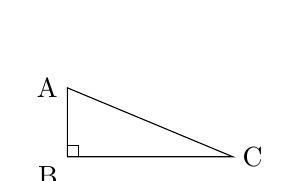
\begin{tikzpicture}[scale=0.35]
\draw (0,2.50) node[left]{A} -- (0,0) node[below left]{B} -- (6.00,0) node[right]{C} -- cycle;
\draw (0,0) rectangle (0.4,0.4);
\end{tikzpicture}
\end{center}

Calculer la valeur exacte de $\ensuremath{\mathrm{A}}\ensuremath{\mathrm{C}}$.

\medskip

\noindent\textbf{2.} Le triangle \ensuremath{\mathrm{D}}\ensuremath{\mathrm{E}}\ensuremath{\mathrm{F}} est rectangle en \ensuremath{\mathrm{E}}. On donne $\ensuremath{\mathrm{D}}\ensuremath{\mathrm{F}} = 20~\text{cm}$ et $\ensuremath{\mathrm{D}}\ensuremath{\mathrm{E}} = 12~\text{cm}$.

\begin{center}
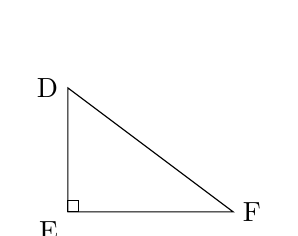
\begin{tikzpicture}[scale=0.35]
\draw (0,4.50) node[left]{D} -- (0,0) node[below left]{E} -- (6.00,0) node[right]{F} -- cycle;
\draw (0,0) rectangle (0.4,0.4);
\end{tikzpicture}
\end{center}

Calculer la valeur exacte de $\ensuremath{\mathrm{E}}\ensuremath{\mathrm{F}}$.

\medskip

\noindent\textbf{3.} Le triangle \ensuremath{\mathrm{M}}\ensuremath{\mathrm{N}}\ensuremath{\mathrm{P}} est rectangle en \ensuremath{\mathrm{N}}. On donne $\ensuremath{\mathrm{M}}\ensuremath{\mathrm{N}} = 8~\text{cm}$ et $\ensuremath{\mathrm{N}}\ensuremath{\mathrm{P}} = 11~\text{cm}$.

\begin{center}
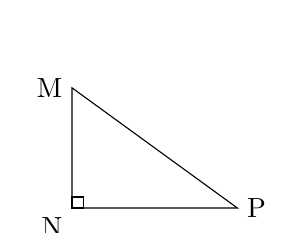
\begin{tikzpicture}[scale=0.35]
\draw (0,4.36) node[left]{M} -- (0,0) node[below left]{N} -- (6.00,0) node[right]{P} -- cycle;
\draw (0,0) rectangle (0.4,0.4);
\end{tikzpicture}
\end{center}

Calculer la valeur exacte de $\ensuremath{\mathrm{M}}\ensuremath{\mathrm{P}}$.

\medskip

\noindent\textbf{4.} Le triangle \ensuremath{\mathrm{R}}\ensuremath{\mathrm{S}}\ensuremath{\mathrm{T}} est rectangle en \ensuremath{\mathrm{S}}. On donne $\ensuremath{\mathrm{R}}\ensuremath{\mathrm{T}} = 10~\text{cm}$ et $\ensuremath{\mathrm{R}}\ensuremath{\mathrm{S}} = 4~\text{cm}$.

\begin{center}
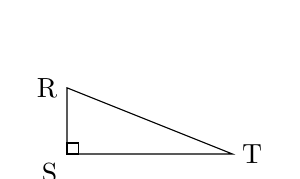
\begin{tikzpicture}[scale=0.35]
\draw (0,2.40) node[left]{R} -- (0,0) node[below left]{S} -- (6.00,0) node[right]{T} -- cycle;
\draw (0,0) rectangle (0.4,0.4);
\end{tikzpicture}
\end{center}

Calculer la valeur exacte de $\ensuremath{\mathrm{S}}\ensuremath{\mathrm{T}}$.

\medskip
\bigskip

\noindent\textbf{Exercice 7} -- Théorème de Thalès

\medskip
\noindent\textbf{1.} Les droites (\ensuremath{\mathrm{B}}\ensuremath{\mathrm{B}^\prime}) et (\ensuremath{\mathrm{C}}\ensuremath{\mathrm{C}^\prime}) sont parallèles. \ensuremath{\mathrm{A}}\ensuremath{\mathrm{B}} = 4, \ensuremath{\mathrm{A}}\ensuremath{\mathrm{B}^\prime} = 3, \ensuremath{\mathrm{A}}\ensuremath{\mathrm{C}} = 7.

\begin{center}
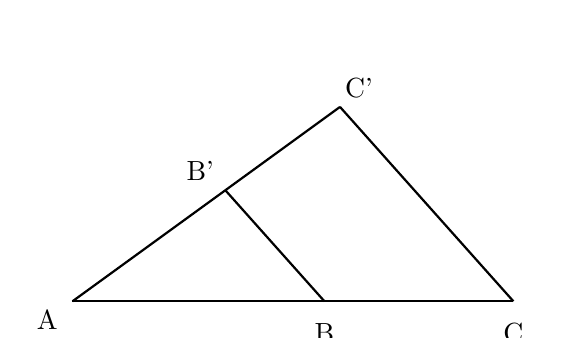
\begin{tikzpicture}[scale=0.8]
\draw [thick] (0.000,0.000)--(4.000,0.000);
\draw [thick] (4.000,0.000)--(7.000,0.000);
\draw [thick] (0.000,0.000)--(2.427,1.763);
\draw [thick] (2.427,1.763)--(4.247,3.086);
\draw [thick] (4.000,0.000)--(2.427,1.763);
\draw [thick] (7.000,0.000)--(4.247,3.086);
\draw (-0.400,-0.300) node {A};
\draw (4.000,-0.500) node {B};
\draw (7.000,-0.500) node {C};
\draw (2.027,2.063) node {B'};
\draw (4.547,3.386) node {C'};
\end{tikzpicture}
\end{center}
Déterminer en justifiant la valeur exacte de \ensuremath{\mathrm{A}}\ensuremath{\mathrm{C}^\prime}.

\bigskip
\noindent\textbf{2.} Les droites (\ensuremath{\mathrm{B}}\ensuremath{\mathrm{B}^\prime}) et (\ensuremath{\mathrm{C}}\ensuremath{\mathrm{C}^\prime}) sont parallèles. \ensuremath{\mathrm{A}}\ensuremath{\mathrm{B}} = 2, \ensuremath{\mathrm{A}}\ensuremath{\mathrm{C}} = 5, \ensuremath{\mathrm{A}}\ensuremath{\mathrm{B}^\prime} = 5.

\begin{center}
\begin{tikzpicture}[scale=0.8]
\draw [thick] (0.000,0.000)--(2.000,0.000);
\draw [thick] (2.000,0.000)--(5.000,0.000);
\draw [thick] (0.000,0.000)--(3.536,3.536);
\draw [thick] (3.536,3.536)--(8.839,8.839);
\draw [thick] (2.000,0.000)--(3.536,3.536);
\draw [thick] (5.000,0.000)--(8.839,8.839);
\draw (-0.400,-0.300) node {A};
\draw (2.000,-0.500) node {B};
\draw (5.000,-0.500) node {C};
\draw (3.136,3.836) node {B'};
\draw (9.139,9.139) node {C'};
\end{tikzpicture}
\end{center}
Déterminer en justifiant la valeur exacte de \ensuremath{\mathrm{A}}\ensuremath{\mathrm{C}^\prime}.

\bigskip
\noindent\textbf{3.} Les droites (\ensuremath{\mathrm{B}}\ensuremath{\mathrm{B}^\prime}) et (\ensuremath{\mathrm{C}}\ensuremath{\mathrm{C}^\prime}) sont parallèles. \ensuremath{\mathrm{A}}\ensuremath{\mathrm{B}} = 4, \ensuremath{\mathrm{A}}\ensuremath{\mathrm{B}^\prime} = 3, \ensuremath{\mathrm{A}}\ensuremath{\mathrm{C}} = 6.

\begin{center}
\begin{tikzpicture}[scale=0.8]
\draw [thick] (0.000,0.000)--(4.000,0.000);
\draw [thick] (4.000,0.000)--(-6.000,0.000);
\draw [thick] (0.000,0.000)--(2.598,1.500);
\draw [thick] (2.598,1.500)--(-3.897,-2.250);
\draw [thick] (4.000,0.000)--(2.598,1.500);
\draw [thick] (-6.000,0.000)--(-3.897,-2.250);
\draw (0.100,-0.500) node {A};
\draw (4.300,0.000) node {B};
\draw (-6.500,0.000) node {C};
\draw (2.898,1.700) node {B'};
\draw (-4.397,-2.450) node {C'};
\end{tikzpicture}
\end{center}
Déterminer en justifiant la valeur exacte de \ensuremath{\mathrm{A}}\ensuremath{\mathrm{C}^\prime}.

\bigskip
\noindent\textbf{4.} Les droites (\ensuremath{\mathrm{B}}\ensuremath{\mathrm{B}^\prime}) et (\ensuremath{\mathrm{C}}\ensuremath{\mathrm{C}^\prime}) sont parallèles. \ensuremath{\mathrm{A}}\ensuremath{\mathrm{B}} = 5, \ensuremath{\mathrm{A}}\ensuremath{\mathrm{B}^\prime} = 2, \ensuremath{\mathrm{A}}\ensuremath{\mathrm{C}} = 8.

\begin{center}
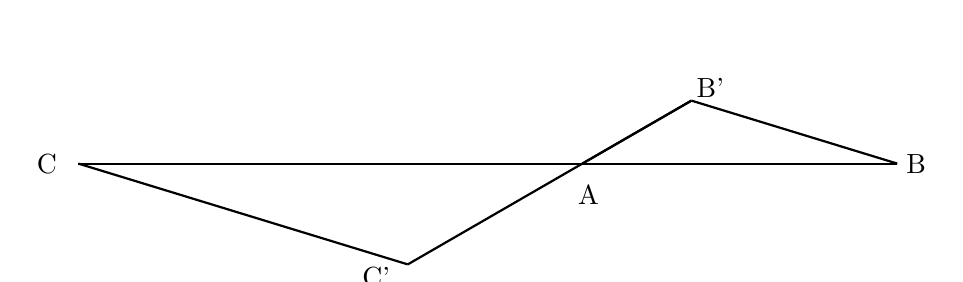
\begin{tikzpicture}[scale=0.8]
\draw [thick] (0.000,0.000)--(5.000,0.000);
\draw [thick] (5.000,0.000)--(-8.000,0.000);
\draw [thick] (0.000,0.000)--(1.732,1.000);
\draw [thick] (1.732,1.000)--(-2.771,-1.600);
\draw [thick] (5.000,0.000)--(1.732,1.000);
\draw [thick] (-8.000,0.000)--(-2.771,-1.600);
\draw (0.100,-0.500) node {A};
\draw (5.300,0.000) node {B};
\draw (-8.500,0.000) node {C};
\draw (2.032,1.200) node {B'};
\draw (-3.271,-1.800) node {C'};
\end{tikzpicture}
\end{center}
Déterminer en justifiant la valeur exacte de \ensuremath{\mathrm{A}}\ensuremath{\mathrm{C}^\prime}.
\bigskip

\noindent\textbf{Exercice 8} -- Résoudre les équations suivantes.
\begin{enumerate}
\item $-7x = 18$
\item $-4x - 4 = 14$
\item $9x + 15 = 2$
\item $-7x - 7 = 9x - 11$
\item $2x + 2 = 3 - 3x$
\end{enumerate}
\bigskip

\noindent\textbf{Exercice 9} -- Résoudre les équations suivantes.
\begin{enumerate}
\item $(6 - 3x)(-6x - 2) = 0$
\item $(2 - 6x)(6x - 2) = 0$
\item $(x + 7)(5x + 5) = 0$
\item $(-x - 1)(x + 6) = 0$
\end{enumerate}
\bigskip

\noindent\textbf{Exercice 10} -- Calculer et simplifier.
\begin{enumerate}
\item $\dfrac{7}{5} - \dfrac{10}{8}$
\item $\dfrac{1}{7} - \dfrac{8}{2}$
\item $\dfrac{4}{3} - \dfrac{1}{6} \times \dfrac{1}{5}$
\item $\dfrac{3}{5} - \dfrac{4}{5} \times \dfrac{4}{2}$
\item $\dfrac{5 + \dfrac{5}{4}}{\dfrac{2}{3} - \dfrac{3}{5}}$
\end{enumerate}
\bigskip

\noindent\textbf{Exercice 11} -- Factoriser les expressions suivantes.
\begin{enumerate}
\item $(x - 2)(-7x - 2) - (x - 2)(3x - 7)$
\item $(-3x - 3)(2x + 7) - (-3x - 3)(7 - 4x)$
\item $(4 - 3x)(-7x - 2) - (4 - 3x)(6x + 3)$
\end{enumerate}
\bigskip

\noindent\textbf{Exercice 12} -- Factoriser en utilisant une identité remarquable.
\begin{enumerate}
\item $(x - 5)^2 - (5x + 7)^2$
\item $4x^2 - 20x + 25$
\item $(x + 7)^2 - (3x + 7)^2$
\end{enumerate}
\bigskip

\noindent\textbf{Exercice 13} -- Résoudre les inéquations suivantes.
\begin{enumerate}
\item $- 4 x \leq -8$
\item $- 8 x \geq -8$
\item $2 x + 8 \leq -3$
\item $- 5 x - 5 \leq -9$
\item $5 x - 7 < 6 x + 9$
\item $- 4 x - 7 \leq 8 x - 5$
\end{enumerate}
\bigskip

\noindent\textbf{Exercice 14} -- Résoudre à l'aide d'un tableau de signes.
\begin{enumerate}
\item $\dfrac{- x - 6}{2 x + 7} \leq 0$
\item $\dfrac{4 x + 1}{2 x - 6} \geq 0$
\item $\left(1 - x\right) \left(2 x - 4\right) < 0$
\item $\dfrac{4 x - 3}{2 x + 8} > 0$
\end{enumerate}
\bigskip

\noindent\textbf{Exercice 15} -- Écrire sous la forme d'une unique puissance de 10.
\begin{enumerate}
\item $\dfrac{10^{-3} \times 10^{3}}{10^{4}}$
\item $\dfrac{10^{0} \times (10^{2})^{3}}{10^{3}}$
\item $\dfrac{10^{-2} \times 10^{-2}}{10^{3}}$
\item $\dfrac{10^{-3} \times (10^{2})^{2}}{10^{2}}$
\end{enumerate}
\bigskip

\noindent\textbf{Exercice 16} -- Calculer et simplifier.
\begin{enumerate}
\item $\sqrt{22050}$
\item $\sqrt{6300}$
\item $5\sqrt{10} + 4\sqrt{3} + 4\sqrt{10} - 4\sqrt{3}$
\item $\sqrt{10} + 3\sqrt{7} + 5\sqrt{10} - 2\sqrt{7}$
\item $\sqrt{48} + 3\sqrt{12} - \sqrt{3} - \sqrt{27}$
\item $(1 - \sqrt{2})^2$
\end{enumerate}
\bigskip

\noindent\textbf{Exercice 17} -- Vecteurs et coordonnées.\\
\medskip
\noindent\textbf{1)} Calculer les coordonnées de $\overrightarrow{\ensuremath{\mathrm{A}}\ensuremath{\mathrm{B}}}$.
\begin{enumerate}
\item $\ensuremath{\mathrm{A}}(4\,;\,-3)$ et $\ensuremath{\mathrm{B}}(-4\,;\,-2)$
\item $\ensuremath{\mathrm{A}}(5\,;\,2)$ et $\ensuremath{\mathrm{B}}(0\,;\,4)$
\item $\ensuremath{\mathrm{A}}(-1\,;\,3)$ et $\ensuremath{\mathrm{B}}(-3\,;\,-3)$
\end{enumerate}
\medskip
\noindent\textbf{2)} Calculer les coordonnées du milieu de $[\ensuremath{\mathrm{A}}\ensuremath{\mathrm{B}}]$.
\begin{enumerate}
\item $\ensuremath{\mathrm{A}}(-3\,;\,6)$ et $\ensuremath{\mathrm{B}}(4\,;\,-4)$
\item $\ensuremath{\mathrm{A}}(6\,;\,5)$ et $\ensuremath{\mathrm{B}}(-8\,;\,0)$
\end{enumerate}
\medskip
\noindent\textbf{3)} Les vecteurs $\vec{u}$ et $\vec{v}$ sont-ils colinéaires ?
\begin{enumerate}
\item $\vec{u}(-4\,;\,3)$ et $\vec{v}(-4\,;\,3)$
\item $\vec{u}(4\,;\,-1)$ et $\vec{v}(-1\,;\,-4)$
\end{enumerate}
\bigskip

\noindent\textbf{Exercice 18} -- Équations de droites.
\medskip
\noindent\textbf{1)} Déterminer l'équation réduite de la droite $(\ensuremath{\mathrm{A}}\ensuremath{\mathrm{B}})$.
\begin{enumerate}
\item $\ensuremath{\mathrm{A}}(-4\,;\,-1)$ et $\ensuremath{\mathrm{B}}(3\,;\,-3)$
\item $\ensuremath{\mathrm{A}}(-5\,;\,0)$ et $\ensuremath{\mathrm{B}}(4\,;\,3)$
\item $\ensuremath{\mathrm{A}}(4\,;\,2)$ et $\ensuremath{\mathrm{B}}(5\,;\,4)$
\end{enumerate}
\noindent\textbf{2)} Déterminer le point d'intersection.
\begin{enumerate}
\item $(d_1): y = -3x$ et $(d_2): y = 4x + 1$
\item $(d_1): y = -5x - 1$ et $(d_2): y = 3x - 2$
\end{enumerate}
\bigskip

\vfill
\begin{flushright}
\qrset{height=1.5cm}
\qrset{level=M}
\qrcode{Ex1: -24x - 12 | -32x + 32 | 18x + 12 | 20x - 4 | 9(-8x - 8) | 2(-7x - 6) | 7(2x + 5) | 6(9x - 9)  //  Ex2: -15 | 63 | 138 | 176 | 60 | 48  //  Ex3: 13 | -12 | -32 | 4 | 2 | -4 | 13 | -18  //  Ex4: 56x^2 + 16x | -9x^2 + 21x | 64x^2 + 136x + 72 | -56x^2 + 65x - 14 | -63x^2 + 8x + 15 | -20x^2 - 66x - 54  //  Ex5: 11 | -3x - 5 | 16 - 7x | 15 - 3x | 13 - x  //  Ex6: sqrt(1521)~ cm | sqrt(256)~ cm | sqrt(185)$ cm | sqrt(84)$ cm  //  Ex7: 21/4 | 25/2 | 9/2 | 16/5  //  Ex8: S = - (18)/(7) | S = - (9)/(2) | S = - (13)/(9) | S = (1)/(4) | S = (1)/(5)  //  Ex9: S = - (1)/(3) ; 2 | S = (1)/(3) | S = -7 ; -1 | S = -6 ; -1  //  Ex10: (3)/(20) | - (27)/(7) | (13)/(10) | -1 | (375)/(4)  //  Ex11: (x - 2)(5 - 10x) | (-3x - 3)(6x) | (4 - 3x)(-13x - 5)  //  Ex12: -8(x + 3)(3x + 1) | (2x - 5)^2 | -4x(2x + 7)  //  Ex13: [ 2 ; +inf [ | ] -inf ; 1 ] | ] -inf ; - (11)/(2) ] | [ (4)/(5) ; +inf [ | ] -16 ; +inf [ | [ - (1)/(6) ; +inf [  //  Ex14: ] -inf ; -6 ] U ] - (7)/(2) ; +inf [ | ] -inf ; - (1)/(4) ] U ] 3 ; +inf [ | ] -inf ; 1 [ U ] 2 ; +inf [ | ] -inf ; -4 [ U ] (3)/(4) ; +inf [  //  Ex15: 10^-4 | 10^3 | 10^-7 | 10^-1  //  Ex16: 105 sqrt(2) | 30 sqrt(7) | 9 sqrt(10) | sqrt(7) + 6 sqrt(10) | 6 sqrt(3) | 3 - 2 sqrt(2)  //  Ex17: AB(-8;1) | AB(-5;2) | AB(-2;-6)  //  Ex18: y = - (2)/(7)x - (15)/(7) | y = (1)/(3)x + (5)/(3) | y = 2x - 6}
\end{flushright}
\newpage
\begin{center}
\textbf{Corrigé numéro 1}\\
\end{center}

\noindent\textbf{Exercice 1}\par
\smallskip
\begin{enumerate}
\item $-3(8x + 4) = -24x - 12$
\item $-8(4x - 4) = -32x + 32$
\item $-2(-9x - 6) = 18x + 12$
\item $4(5x - 1) = 20x - 4$
\end{enumerate}
\begin{enumerate}
\item $-72x - 72 = 9(-8x - 8)$
\item $-14x - 12 = 2(-7x - 6)$
\item $14x + 35 = 7(2x + 5)$
\item $54x - 54 = 6(9x - 9)$
\end{enumerate}
\medskip

\noindent\textbf{Exercice 2}\par
\smallskip
\begin{enumerate}
\item $9 \times (7 - 9) + 3$

$= 9 \times -2 + 3$

$= -18 + 3$

$= -15$
\item $(10 - 3) \times 9$

$= 7 \times 9$

$= 63$
\item $(13 + 10) \times 6$

$= 23 \times 6$

$= 138$
\item $(13 + 9) \times 8$

$= 22 \times 8$

$= 176$
\item $6 \times (6 + 3) + 6$

$= 6 \times 9 + 6$

$= 54 + 6$

$= 60$
\item $(7 + 1) \times 6$

$= 8 \times 6$

$= 48$
\end{enumerate}
\medskip

\noindent\textbf{Exercice 3}\par
\smallskip
\begin{enumerate}
\item $(+6) + (+12) + (-5) = 13$
\item $(-17) + (+7) + (-2) = -12$
\item $(-17) + (-7) + (-8) = -32$
\item $(-5) + (+19) + (-10) = 4$
\item $(-16) - (-16) - (-2) = 2$
\item $(-5) + (+3) - (+2) = -4$
\item $(+1) - (+6) - (-18) = 13$
\item $(+3) + (-11) - (+10) = -18$
\end{enumerate}
\medskip

\noindent\textbf{Exercice 4}\par
\smallskip
\begin{enumerate}
\item $8x(7x + 2) = 56x^2 + 16x$
\item $3x(7 - 3x) = -9x^2 + 21x$
\item $(8x + 8)(8x + 9) = 64x^2 + 136x + 72$
\item $(2 - 7x)(8x - 7) = -56x^2 + 65x - 14$
\item $(5 - 9x)(7x + 3) = -63x^2 + 8x + 15$
\item $(-5x - 9)(4x + 6) = -20x^2 - 66x - 54$
\end{enumerate}
\medskip

\noindent\textbf{Exercice 5}\par
\smallskip
\begin{enumerate}
\item $(6 - 3x)-(-3x - 5) = 11$
\item $(-6x - 3)-(2 - 3x) = -3x - 5$
\item $-(4x - 9)-(3x - 7) = 16 - 7x$
\item $-(6x - 7)-(-3x - 8) = 15 - 3x$
\item $(4 - 5x)+(4x + 9) = 13 - x$
\end{enumerate}
\medskip

\noindent\textbf{Exercice 6}\par
\smallskip
\textbf{1.} D'après le théorème de Pythagore dans le triangle \ensuremath{\mathrm{A}}\ensuremath{\mathrm{B}}\ensuremath{\mathrm{C}} rectangle en \ensuremath{\mathrm{B}} :

$\ensuremath{\mathrm{A}}\ensuremath{\mathrm{C}}^2 = \ensuremath{\mathrm{A}}\ensuremath{\mathrm{B}}^2 + \ensuremath{\mathrm{B}}\ensuremath{\mathrm{C}}^2$

$\ensuremath{\mathrm{A}}\ensuremath{\mathrm{C}}^2 = (15~\text{cm})^2 + (36~\text{cm})^2 = 225~\text{cm}^2 + 1296~\text{cm}^2 = 1521~\text{cm}^2$

Donc $\ensuremath{\mathrm{A}}\ensuremath{\mathrm{C}} = \sqrt{1521}~\text{cm} = 39~\text{cm}$

\medskip
\textbf{2.} D'après le théorème de Pythagore dans le triangle \ensuremath{\mathrm{D}}\ensuremath{\mathrm{E}}\ensuremath{\mathrm{F}} rectangle en \ensuremath{\mathrm{E}} :

$\ensuremath{\mathrm{D}}\ensuremath{\mathrm{F}}^2 = \ensuremath{\mathrm{D}}\ensuremath{\mathrm{E}}^2 + \ensuremath{\mathrm{E}}\ensuremath{\mathrm{F}}^2$

Donc $\ensuremath{\mathrm{E}}\ensuremath{\mathrm{F}}^2 = \ensuremath{\mathrm{D}}\ensuremath{\mathrm{F}}^2 - \ensuremath{\mathrm{D}}\ensuremath{\mathrm{E}}^2 = (20~\text{cm})^2 - (12~\text{cm})^2 = 400~\text{cm}^2 - 144~\text{cm}^2 = 256~\text{cm}^2$

Donc $\ensuremath{\mathrm{E}}\ensuremath{\mathrm{F}} = \sqrt{256}~\text{cm} = 16~\text{cm}$

\medskip
\textbf{3.} D'après le théorème de Pythagore :

$\ensuremath{\mathrm{M}}\ensuremath{\mathrm{P}}^2 = (8~\text{cm})^2 + (11~\text{cm})^2 = 64~\text{cm}^2 + 121~\text{cm}^2 = 185~\text{cm}^2$

Donc $\ensuremath{\mathrm{M}}\ensuremath{\mathrm{P}} = \sqrt{185}$ cm

\medskip
\textbf{4.} D'après le théorème de Pythagore :

$\ensuremath{\mathrm{R}}\ensuremath{\mathrm{T}}^2 = \ensuremath{\mathrm{R}}\ensuremath{\mathrm{S}}^2 + \ensuremath{\mathrm{S}}\ensuremath{\mathrm{T}}^2$

Donc $\ensuremath{\mathrm{S}}\ensuremath{\mathrm{T}}^2 = (10~\text{cm})^2 - (4~\text{cm})^2 = 100~\text{cm}^2 - 16~\text{cm}^2 = 84~\text{cm}^2$

Donc $\ensuremath{\mathrm{S}}\ensuremath{\mathrm{T}} = \sqrt{84}$ cm

\medskip
\medskip

\noindent\textbf{Exercice 7}\par
\smallskip
\textbf{1.} Comme (\ensuremath{\mathrm{B}}\ensuremath{\mathrm{B}^\prime}) et (\ensuremath{\mathrm{C}}\ensuremath{\mathrm{C}^\prime}) sont parallèles, d'après le théorème de Thalès : \[\dfrac{\ensuremath{\mathrm{A}}\ensuremath{\mathrm{C}^\prime}}{\ensuremath{\mathrm{A}}\ensuremath{\mathrm{C}}}=\dfrac{\ensuremath{\mathrm{A}}\ensuremath{\mathrm{B}^\prime}}{\ensuremath{\mathrm{A}}\ensuremath{\mathrm{B}}}=\dfrac{3}{4}.\]Donc \[\ensuremath{\mathrm{A}}\ensuremath{\mathrm{C}^\prime}=7\times\dfrac{3}{4}=\dfrac{21}{4}.\]\medskip
\textbf{2.} Comme (\ensuremath{\mathrm{B}}\ensuremath{\mathrm{B}^\prime}) et (\ensuremath{\mathrm{C}}\ensuremath{\mathrm{C}^\prime}) sont parallèles, d'après le théorème de Thalès : \[\dfrac{\ensuremath{\mathrm{A}}\ensuremath{\mathrm{C}^\prime}}{\ensuremath{\mathrm{A}}\ensuremath{\mathrm{C}}}=\dfrac{\ensuremath{\mathrm{A}}\ensuremath{\mathrm{B}^\prime}}{\ensuremath{\mathrm{A}}\ensuremath{\mathrm{B}}}=\dfrac{5}{2}.\]Donc \[\ensuremath{\mathrm{A}}\ensuremath{\mathrm{C}^\prime}=5\times\dfrac{5}{2}=\dfrac{25}{2}.\]\medskip
\textbf{3.} Comme (\ensuremath{\mathrm{B}}\ensuremath{\mathrm{B}^\prime}) et (\ensuremath{\mathrm{C}}\ensuremath{\mathrm{C}^\prime}) sont parallèles, d'après le théorème de Thalès : \[\dfrac{\ensuremath{\mathrm{A}}\ensuremath{\mathrm{C}^\prime}}{\ensuremath{\mathrm{A}}\ensuremath{\mathrm{C}}}=\dfrac{\ensuremath{\mathrm{A}}\ensuremath{\mathrm{B}^\prime}}{\ensuremath{\mathrm{A}}\ensuremath{\mathrm{B}}}=\dfrac{3}{4}.\]Donc \[\ensuremath{\mathrm{A}}\ensuremath{\mathrm{C}^\prime}=6\times\dfrac{3}{4}=\dfrac{9}{2}.\]\medskip
\textbf{4.} Comme (\ensuremath{\mathrm{B}}\ensuremath{\mathrm{B}^\prime}) et (\ensuremath{\mathrm{C}}\ensuremath{\mathrm{C}^\prime}) sont parallèles, d'après le théorème de Thalès : \[\dfrac{\ensuremath{\mathrm{A}}\ensuremath{\mathrm{C}^\prime}}{\ensuremath{\mathrm{A}}\ensuremath{\mathrm{C}}}=\dfrac{\ensuremath{\mathrm{A}}\ensuremath{\mathrm{B}^\prime}}{\ensuremath{\mathrm{A}}\ensuremath{\mathrm{B}}}=\dfrac{2}{5}.\]Donc \[\ensuremath{\mathrm{A}}\ensuremath{\mathrm{C}^\prime}=8\times\dfrac{2}{5}=\dfrac{16}{5}.\]\medskip
\medskip

\noindent\textbf{Exercice 8}\par
\smallskip
\begin{enumerate}
\item $-7x = 18$

$\Leftrightarrow x = \dfrac{18}{-7} = - \dfrac{18}{7}$

L'ensemble des solutions est $S = \left\{- \dfrac{18}{7}\right\}$.

\item $-4x - 4 = 14$

$\Leftrightarrow -4x = 14 - (-4) = 18$

$\Leftrightarrow x = \dfrac{18}{-4} = - \dfrac{9}{2}$

L'ensemble des solutions est $S = \left\{- \dfrac{9}{2}\right\}$.

\item $9x + 15 = 2$

$\Leftrightarrow 9x = 2 - (15) = -13$

$\Leftrightarrow x = \dfrac{-13}{9} = - \dfrac{13}{9}$

L'ensemble des solutions est $S = \left\{- \dfrac{13}{9}\right\}$.

\item $-7x - 7 = 9x - 11$

$\Leftrightarrow -16x = -4$

$\Leftrightarrow x = \dfrac{-4}{-16} = \dfrac{1}{4}$

L'ensemble des solutions est $S = \left\{\dfrac{1}{4}\right\}$.

\item $2x + 2 = 3 - 3x$

$\Leftrightarrow 5x = 1$

$\Leftrightarrow x = \dfrac{1}{5} = \dfrac{1}{5}$

L'ensemble des solutions est $S = \left\{\dfrac{1}{5}\right\}$.

\end{enumerate}
\medskip

\noindent\textbf{Exercice 9}\par
\smallskip
\begin{enumerate}
\item Un produit est nul si et seulement si l'un des facteurs est nul.

$\bullet\ -6x - 2 = 0 \Leftrightarrow x = - \dfrac{1}{3}$

$\bullet\ 6 - 3x = 0 \Leftrightarrow x = 2$

Donc $S = \left\{- \dfrac{1}{3} \; ; \; 2\right\}$

\item Un produit est nul si et seulement si l'un des facteurs est nul.

$\bullet\ 6x - 2 = 0 \Leftrightarrow x = \dfrac{1}{3}$

$\bullet\ 2 - 6x = 0 \Leftrightarrow x = \dfrac{1}{3}$

Donc $S = \left\{\dfrac{1}{3}\right\}$

\item Un produit est nul si et seulement si l'un des facteurs est nul.

$\bullet\ 5x + 5 = 0 \Leftrightarrow x = -1$

$\bullet\ x + 7 = 0 \Leftrightarrow x = -7$

Donc $S = \left\{-7 \; ; \; -1\right\}$

\item Un produit est nul si et seulement si l'un des facteurs est nul.

$\bullet\ x + 6 = 0 \Leftrightarrow x = -6$

$\bullet\ -x - 1 = 0 \Leftrightarrow x = -1$

Donc $S = \left\{-6 \; ; \; -1\right\}$

\end{enumerate}
\medskip

\noindent\textbf{Exercice 10}\par
\smallskip
\begin{enumerate}
\item $\dfrac{7 \times 8}{5 \times 8} - \dfrac{10 \times 5}{8 \times 5} = \dfrac{6}{40} = \dfrac{3}{20}$
\item $\dfrac{1 \times 2}{7 \times 2} - \dfrac{8 \times 7}{2 \times 7} = \dfrac{-54}{14} = - \dfrac{27}{7}$
\item $= \dfrac{4}{3} - \dfrac{1}{30}$ (priorité $\times$)

$= \dfrac{40}{30} - \dfrac{1}{30} = \dfrac{39}{30}$
\item $= \dfrac{3}{5} - \dfrac{8}{5}$ (priorité $\times$)

$= \dfrac{3 - 8}{5} = -1$
\item Numérateur : $5 + \dfrac{5}{4} = \dfrac{5 \times 4 + 5}{4} = \dfrac{25}{4}$

Dénominateur : $\dfrac{2}{3} - \dfrac{3}{5} = \dfrac{2 \times 5 - 3 \times 3}{3 \times 5} = \dfrac{1}{15}$

$= \dfrac{25}{4} \div \dfrac{1}{15} = \dfrac{25}{4} \times 15 = \dfrac{375}{4}$
\end{enumerate}
\medskip

\noindent\textbf{Exercice 11}\par
\smallskip
\begin{enumerate}
\item $(x - 2)(5 - 10x)$
\item $(-3x - 3)(6x)$
\item $(4 - 3x)(-13x - 5)$
\end{enumerate}
\medskip

\noindent\textbf{Exercice 12}\par
\smallskip
\begin{enumerate}
\item $-8(x + 3)(3x + 1)$
\item $(2x - 5)^2$
\item $-4x(2x + 7)$
\end{enumerate}
\medskip

\noindent\textbf{Exercice 13}\par
\smallskip
\begin{enumerate}
\item $-4x \leq -8$

$\Leftrightarrow x \geq 2$

$S = \left[ 2 \,;\, +\infty \right[$
\item $-8x \geq -8$

$\Leftrightarrow x \leq 1$

$S = \left] -\infty \,;\, 1 \right]$
\item $2 x + 8 \leq -3$

$\Leftrightarrow 2x \leq -3 - (8) = -11$

$\Leftrightarrow x \leq - \dfrac{11}{2}$

$S = \left] -\infty \,;\, - \dfrac{11}{2} \right]$
\item $- 5 x - 5 \leq -9$

$\Leftrightarrow -5x \leq -9 - (-5) = -4$

$\Leftrightarrow x \geq \dfrac{4}{5}$

$S = \left[ \dfrac{4}{5} \,;\, +\infty \right[$
\item $5 x - 7 < 6 x + 9$

$\Leftrightarrow -x < 16$

$\Leftrightarrow x > -16$

$S = \left] -16 \,;\, +\infty \right[$
\item $- 4 x - 7 \leq 8 x - 5$

$\Leftrightarrow -12x \leq 2$

$\Leftrightarrow x \geq - \dfrac{1}{6}$

$S = \left[ - \dfrac{1}{6} \,;\, +\infty \right[$
\end{enumerate}
\medskip

\noindent\textbf{Exercice 14}\par
\smallskip
\noindent\textbf{1)}\par\smallskip
\begin{center}
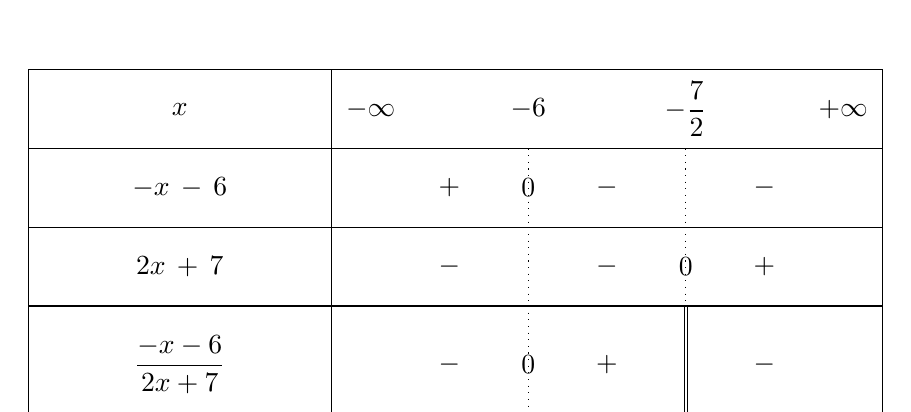
\begin{tikzpicture}
\tkzTabInit[lgt=3.85,espcl=2]{$x$ / 1, $- x - 6$ / 1, $2 x + 7$ / 1, $\dfrac{- x - 6}{2 x + 7}$ / 1.5}{$-\infty$, $-6$, $- \dfrac{7}{2}$, $+\infty$}
\tkzTabLine{, +, z, -, t, -}
\tkzTabLine{, -, t, -, z, +}
\tkzTabLine{, -, z, +, d, -}
\end{tikzpicture}
\end{center}
\par\smallskip
\begin{center}$S = \left] -\infty \,;\, -6 \right] \cup \left] - \dfrac{7}{2} \,;\, +\infty \right[$\end{center}\par\medskip
\noindent\textbf{2)}\par\smallskip
\begin{center}
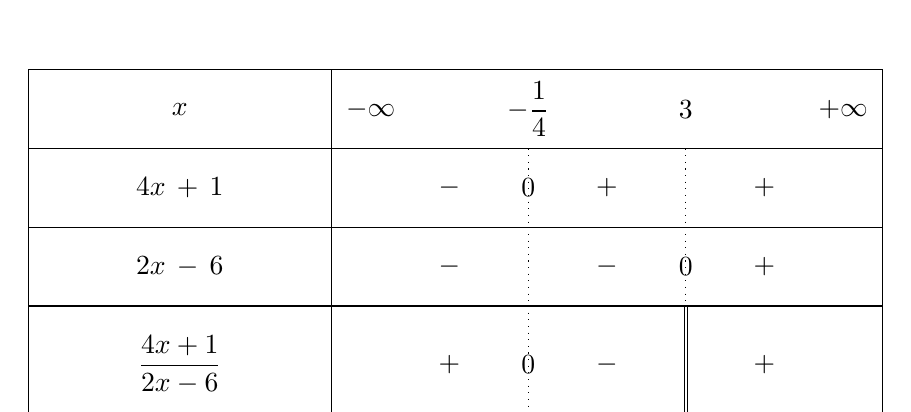
\begin{tikzpicture}
\tkzTabInit[lgt=3.85,espcl=2]{$x$ / 1, $4 x + 1$ / 1, $2 x - 6$ / 1, $\dfrac{4 x + 1}{2 x - 6}$ / 1.5}{$-\infty$, $- \dfrac{1}{4}$, $3$, $+\infty$}
\tkzTabLine{, -, z, +, t, +}
\tkzTabLine{, -, t, -, z, +}
\tkzTabLine{, +, z, -, d, +}
\end{tikzpicture}
\end{center}
\par\smallskip
\begin{center}$S = \left] -\infty \,;\, - \dfrac{1}{4} \right] \cup \left] 3 \,;\, +\infty \right[$\end{center}\par\medskip
\noindent\textbf{3)}\par\smallskip
\begin{center}
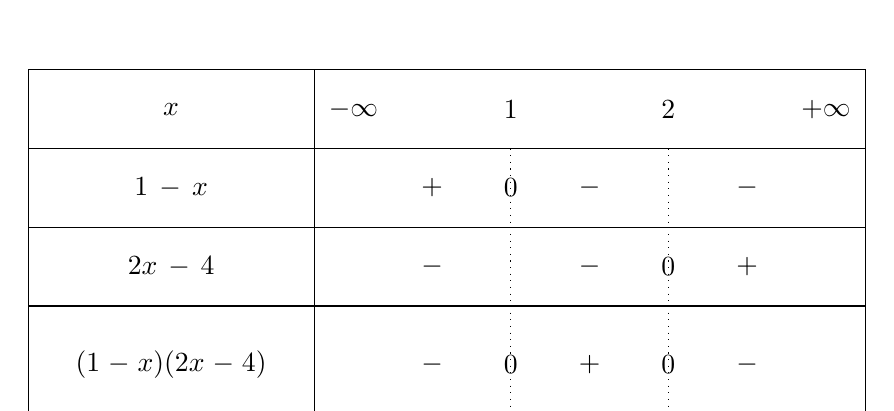
\begin{tikzpicture}
\tkzTabInit[lgt=3.63,espcl=2]{$x$ / 1, $1 - x$ / 1, $2 x - 4$ / 1, $(1 - x)(2 x - 4)$ / 1.5}{$-\infty$, $1$, $2$, $+\infty$}
\tkzTabLine{, +, z, -, t, -}
\tkzTabLine{, -, t, -, z, +}
\tkzTabLine{, -, z, +, z, -}
\end{tikzpicture}
\end{center}
\par\smallskip
\begin{center}$S = \left] -\infty \,;\, 1 \right[ \cup \left] 2 \,;\, +\infty \right[$\end{center}\par\medskip
\noindent\textbf{4)}\par\smallskip
\begin{center}
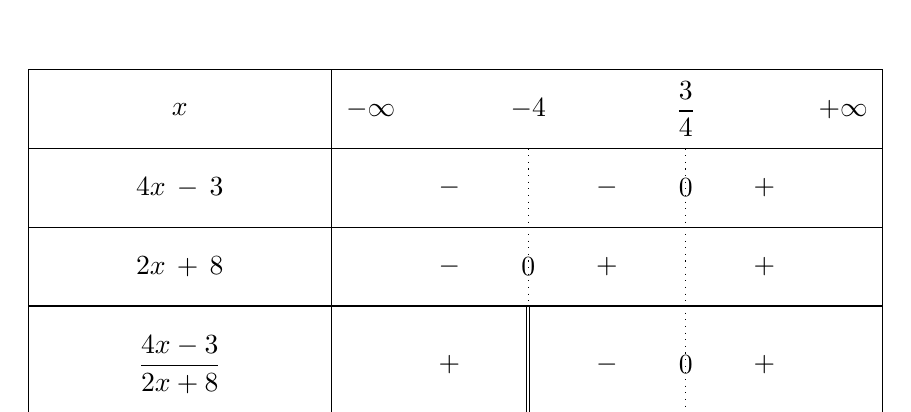
\begin{tikzpicture}
\tkzTabInit[lgt=3.85,espcl=2]{$x$ / 1, $4 x - 3$ / 1, $2 x + 8$ / 1, $\dfrac{4 x - 3}{2 x + 8}$ / 1.5}{$-\infty$, $-4$, $\dfrac{3}{4}$, $+\infty$}
\tkzTabLine{, -, t, -, z, +}
\tkzTabLine{, -, z, +, t, +}
\tkzTabLine{, +, d, -, z, +}
\end{tikzpicture}
\end{center}
\par\smallskip
\begin{center}$S = \left] -\infty \,;\, -4 \right[ \cup \left] \dfrac{3}{4} \,;\, +\infty \right[$\end{center}\par\medskip
\medskip

\noindent\textbf{Exercice 15}\par
\smallskip
\begin{enumerate}
\item $\dfrac{10^{-3} \times 10^{3}}{10^{4}} = 10^{-4}$
\item $\dfrac{10^{0} \times (10^{2})^{3}}{10^{3}} = 10^{3}$
\item $\dfrac{10^{-2} \times 10^{-2}}{10^{3}} = 10^{-7}$
\item $\dfrac{10^{-3} \times (10^{2})^{2}}{10^{2}} = 10^{-1}$
\end{enumerate}
\medskip

\noindent\textbf{Exercice 16}\par
\smallskip
\begin{enumerate}
\item $105 \sqrt{2}$
\item $30 \sqrt{7}$
\item $9 \sqrt{10}$
\item $\sqrt{7} + 6 \sqrt{10}$
\item $6 \sqrt{3}$
\item $3 - 2 \sqrt{2}$
\end{enumerate}
\medskip

\noindent\textbf{Exercice 17}\par
\smallskip
\textbf{1)}
\begin{enumerate}
\item $\overrightarrow{\ensuremath{\mathrm{A}}\ensuremath{\mathrm{B}}}(-8\,;\,1)$
\item $\overrightarrow{\ensuremath{\mathrm{A}}\ensuremath{\mathrm{B}}}(-5\,;\,2)$
\item $\overrightarrow{\ensuremath{\mathrm{A}}\ensuremath{\mathrm{B}}}(-2\,;\,-6)$
\end{enumerate}
\textbf{2)}
\begin{enumerate}
\item $\ensuremath{\mathrm{M}}\left(\dfrac{1}{2}\,;\,1\right)$
\item $\ensuremath{\mathrm{M}}\left(-1\,;\,\dfrac{5}{2}\right)$
\end{enumerate}
\textbf{3)}
\begin{enumerate}
\item $\det(\vec{u},\vec{v}) = -4\times(3)-(3)\times-4 = 0$. Oui.
\item $\det(\vec{u},\vec{v}) = 4\times(-4)-(-1)\times-1 = -17$. Non.
\end{enumerate}
\medskip

\noindent\textbf{Exercice 18}\par
\smallskip
\textbf{1)}
\begin{enumerate}
\item $m = \dfrac{-3--1}{3--4} = - \dfrac{2}{7}$ donc $y = - \dfrac{2}{7}x - \dfrac{15}{7}$
\item $m = \dfrac{3-0}{4--5} = \dfrac{1}{3}$ donc $y = \dfrac{1}{3}x + \dfrac{5}{3}$
\item $m = \dfrac{4-2}{5-4} = 2$ donc $y = 2x - 6$
\end{enumerate}
\textbf{2)}
\begin{enumerate}
\item On cherche les couples $(x\,;\,y)$ vérifiant les deux équations :

$-3x = 4x + 1$

$\Leftrightarrow -7x = 1$

$\Leftrightarrow x = - \dfrac{1}{7}$

puis $y = -3 \times (- \dfrac{1}{7}) = \dfrac{3}{7}$

Donc le point d'intersection est $\left(- \dfrac{1}{7}\,;\,\dfrac{3}{7}\right)$.
\item On cherche les couples $(x\,;\,y)$ vérifiant les deux équations :

$-5x - 1 = 3x - 2$

$\Leftrightarrow -8x = -1$

$\Leftrightarrow x = \dfrac{1}{8}$

puis $y = -5 \times (\dfrac{1}{8}) - 1 = - \dfrac{13}{8}$

Donc le point d'intersection est $\left(\dfrac{1}{8}\,;\,- \dfrac{13}{8}\right)$.
\end{enumerate}
\medskip

\newpage
\begin{center}
\textbf{Sujet numéro 2}
\\(à rendre avec la copie)
\end{center}


\noindent\textbf{Exercice 1} -- Développer les expressions suivantes.
\begin{enumerate}
\item $(8x + 5)$
\item $3(-9x + 8)$
\item $-6(-3x - 6)$
\item $-3(8x - 6)$
\end{enumerate}
\noindent\textbf{Exercice} -- Factoriser les expressions suivantes.
\begin{enumerate}
\item $36x - 18$
\item $81x - 54$
\item $-45x + 36$
\item $-35x + 20$
\end{enumerate}
\bigskip

\noindent\textbf{Exercice 2} -- Calculer en respectant les priorités opératoires.
\begin{enumerate}
\item $3 \times (4 + 7) - 2$
\item $7 \times (8 + 10) - 5$
\item $5 \times (2 + 5) - 6$
\item $9 \times (3 - 7) - 2$
\item $(5 + 4) \times 3$
\item $8 \times (4 - 1) + 6$
\end{enumerate}
\bigskip

\noindent\textbf{Exercice 3} -- Calculer les expressions suivantes.
\begin{enumerate}
\item $(-18) + (+13) + (-9)$
\item $(+16) + (+7) + (-18)$
\item $(-15) + (-19) + (+17)$
\item $(-7) + (+2) + (+15)$
\item $(+10) - (+4) + (+10)$
\item $(+19) - (-13) + (-7)$
\item $(-16) + (-16) - (+13)$
\item $(-12) - (-10) - (-16)$
\end{enumerate}
\bigskip

\noindent\textbf{Exercice 4} -- Développer et réduire.
\begin{enumerate}
\item $-6x(6x - 8)$
\item $6x(7x - 3)$
\item $(-2x - 6)(5x - 7)$
\item $(6x + 9)(8x - 6)$
\item $(3x - 2)(9x + 6)$
\item $(6 - 2x)(9x - 9)$
\end{enumerate}
\bigskip

\noindent\textbf{Exercice 5} -- Réduire les expressions suivantes.
\begin{enumerate}
\item $-(3x + 4)+(6x - 5)$
\item $(-8x - 4)+(-2x - 6)$
\item $-(5x - 4)-(-4x - 8)$
\item $(3x + 7)-(4 - 6x)$
\item $-(-3x - 3)-(7 - 6x)$
\end{enumerate}
\bigskip

\noindent\textbf{Exercice 6} -- Théorème de Pythagore.
\medskip

\noindent\textbf{1.} Le triangle \ensuremath{\mathrm{A}}\ensuremath{\mathrm{B}}\ensuremath{\mathrm{C}} est rectangle en \ensuremath{\mathrm{B}}. On donne $\ensuremath{\mathrm{A}}\ensuremath{\mathrm{B}} = 8~\text{cm}$ et $\ensuremath{\mathrm{B}}\ensuremath{\mathrm{C}} = 15~\text{cm}$.

\begin{center}
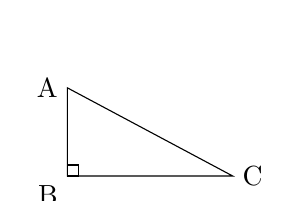
\begin{tikzpicture}[scale=0.35]
\draw (0,3.20) node[left]{A} -- (0,0) node[below left]{B} -- (6.00,0) node[right]{C} -- cycle;
\draw (0,0) rectangle (0.4,0.4);
\end{tikzpicture}
\end{center}

Calculer la valeur exacte de $\ensuremath{\mathrm{A}}\ensuremath{\mathrm{C}}$.

\medskip

\noindent\textbf{2.} Le triangle \ensuremath{\mathrm{D}}\ensuremath{\mathrm{E}}\ensuremath{\mathrm{F}} est rectangle en \ensuremath{\mathrm{E}}. On donne $\ensuremath{\mathrm{D}}\ensuremath{\mathrm{F}} = 17~\text{cm}$ et $\ensuremath{\mathrm{D}}\ensuremath{\mathrm{E}} = 8~\text{cm}$.

\begin{center}
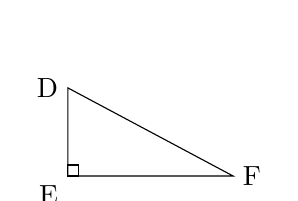
\begin{tikzpicture}[scale=0.35]
\draw (0,3.20) node[left]{D} -- (0,0) node[below left]{E} -- (6.00,0) node[right]{F} -- cycle;
\draw (0,0) rectangle (0.4,0.4);
\end{tikzpicture}
\end{center}

Calculer la valeur exacte de $\ensuremath{\mathrm{E}}\ensuremath{\mathrm{F}}$.

\medskip

\noindent\textbf{3.} Le triangle \ensuremath{\mathrm{M}}\ensuremath{\mathrm{N}}\ensuremath{\mathrm{P}} est rectangle en \ensuremath{\mathrm{N}}. On donne $\ensuremath{\mathrm{M}}\ensuremath{\mathrm{N}} = 2~\text{cm}$ et $\ensuremath{\mathrm{N}}\ensuremath{\mathrm{P}} = 12~\text{cm}$.

\begin{center}
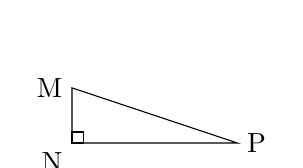
\begin{tikzpicture}[scale=0.35]
\draw (0,2.00) node[left]{M} -- (0,0) node[below left]{N} -- (6.00,0) node[right]{P} -- cycle;
\draw (0,0) rectangle (0.4,0.4);
\end{tikzpicture}
\end{center}

Calculer la valeur exacte de $\ensuremath{\mathrm{M}}\ensuremath{\mathrm{P}}$.

\medskip

\noindent\textbf{4.} Le triangle \ensuremath{\mathrm{R}}\ensuremath{\mathrm{S}}\ensuremath{\mathrm{T}} est rectangle en \ensuremath{\mathrm{S}}. On donne $\ensuremath{\mathrm{R}}\ensuremath{\mathrm{T}} = 11~\text{cm}$ et $\ensuremath{\mathrm{R}}\ensuremath{\mathrm{S}} = 3~\text{cm}$.

\begin{center}
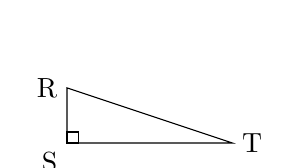
\begin{tikzpicture}[scale=0.35]
\draw (0,2.00) node[left]{R} -- (0,0) node[below left]{S} -- (6.00,0) node[right]{T} -- cycle;
\draw (0,0) rectangle (0.4,0.4);
\end{tikzpicture}
\end{center}

Calculer la valeur exacte de $\ensuremath{\mathrm{S}}\ensuremath{\mathrm{T}}$.

\medskip
\bigskip

\noindent\textbf{Exercice 7} -- Théorème de Thalès

\medskip
\noindent\textbf{1.} Les droites (\ensuremath{\mathrm{B}}\ensuremath{\mathrm{B}^\prime}) et (\ensuremath{\mathrm{C}}\ensuremath{\mathrm{C}^\prime}) sont parallèles. \ensuremath{\mathrm{A}}\ensuremath{\mathrm{B}} = 4, \ensuremath{\mathrm{A}}\ensuremath{\mathrm{B}^\prime} = 3, \ensuremath{\mathrm{A}}\ensuremath{\mathrm{C}} = 7.

\begin{center}
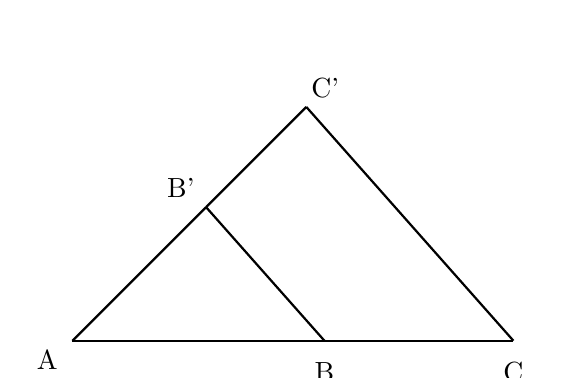
\begin{tikzpicture}[scale=0.8]
\draw [thick] (0.000,0.000)--(4.000,0.000);
\draw [thick] (4.000,0.000)--(7.000,0.000);
\draw [thick] (0.000,0.000)--(2.121,2.121);
\draw [thick] (2.121,2.121)--(3.712,3.712);
\draw [thick] (4.000,0.000)--(2.121,2.121);
\draw [thick] (7.000,0.000)--(3.712,3.712);
\draw (-0.400,-0.300) node {A};
\draw (4.000,-0.500) node {B};
\draw (7.000,-0.500) node {C};
\draw (1.721,2.421) node {B'};
\draw (4.012,4.012) node {C'};
\end{tikzpicture}
\end{center}
Déterminer en justifiant la valeur exacte de \ensuremath{\mathrm{A}}\ensuremath{\mathrm{C}^\prime}.

\bigskip
\noindent\textbf{2.} Les droites (\ensuremath{\mathrm{B}}\ensuremath{\mathrm{B}^\prime}) et (\ensuremath{\mathrm{C}}\ensuremath{\mathrm{C}^\prime}) sont parallèles. \ensuremath{\mathrm{A}}\ensuremath{\mathrm{B}} = 2, \ensuremath{\mathrm{A}}\ensuremath{\mathrm{C}} = 4, \ensuremath{\mathrm{A}}\ensuremath{\mathrm{B}^\prime} = 4.

\begin{center}
\begin{tikzpicture}[scale=0.8]
\draw [thick] (0.000,0.000)--(2.000,0.000);
\draw [thick] (2.000,0.000)--(4.000,0.000);
\draw [thick] (0.000,0.000)--(2.828,2.828);
\draw [thick] (2.828,2.828)--(5.657,5.657);
\draw [thick] (2.000,0.000)--(2.828,2.828);
\draw [thick] (4.000,0.000)--(5.657,5.657);
\draw (-0.400,-0.300) node {A};
\draw (2.000,-0.500) node {B};
\draw (4.000,-0.500) node {C};
\draw (2.428,3.128) node {B'};
\draw (5.957,5.957) node {C'};
\end{tikzpicture}
\end{center}
Déterminer en justifiant la valeur exacte de \ensuremath{\mathrm{A}}\ensuremath{\mathrm{C}^\prime}.

\bigskip
\noindent\textbf{3.} Les droites (\ensuremath{\mathrm{B}}\ensuremath{\mathrm{B}^\prime}) et (\ensuremath{\mathrm{C}}\ensuremath{\mathrm{C}^\prime}) sont parallèles. \ensuremath{\mathrm{A}}\ensuremath{\mathrm{C}} = 6, \ensuremath{\mathrm{A}}\ensuremath{\mathrm{B}^\prime} = 3, \ensuremath{\mathrm{A}}\ensuremath{\mathrm{B}} = 4.

\begin{center}
\begin{tikzpicture}[scale=0.8]
\draw [thick] (0.000,0.000)--(4.000,0.000);
\draw [thick] (4.000,0.000)--(-6.000,0.000);
\draw [thick] (0.000,0.000)--(2.427,1.763);
\draw [thick] (2.427,1.763)--(-3.641,-2.645);
\draw [thick] (4.000,0.000)--(2.427,1.763);
\draw [thick] (-6.000,0.000)--(-3.641,-2.645);
\draw (0.100,-0.500) node {A};
\draw (4.300,0.000) node {B};
\draw (-6.500,0.000) node {C};
\draw (2.727,1.963) node {B'};
\draw (-4.141,-2.845) node {C'};
\end{tikzpicture}
\end{center}
Déterminer en justifiant la valeur exacte de \ensuremath{\mathrm{A}}\ensuremath{\mathrm{C}^\prime}.

\bigskip
\noindent\textbf{4.} Les droites (\ensuremath{\mathrm{B}}\ensuremath{\mathrm{B}^\prime}) et (\ensuremath{\mathrm{C}}\ensuremath{\mathrm{C}^\prime}) sont parallèles. \ensuremath{\mathrm{A}}\ensuremath{\mathrm{B}^\prime} = 5, \ensuremath{\mathrm{A}}\ensuremath{\mathrm{B}} = 2, \ensuremath{\mathrm{A}}\ensuremath{\mathrm{C}} = 5.

\begin{center}
\begin{tikzpicture}[scale=0.8]
\draw [thick] (0.000,0.000)--(2.000,0.000);
\draw [thick] (2.000,0.000)--(-5.000,0.000);
\draw [thick] (0.000,0.000)--(3.536,3.536);
\draw [thick] (3.536,3.536)--(-8.839,-8.839);
\draw [thick] (2.000,0.000)--(3.536,3.536);
\draw [thick] (-5.000,0.000)--(-8.839,-8.839);
\draw (0.100,-0.500) node {A};
\draw (2.300,0.000) node {B};
\draw (-5.500,0.000) node {C};
\draw (3.836,3.736) node {B'};
\draw (-9.339,-9.039) node {C'};
\end{tikzpicture}
\end{center}
Déterminer en justifiant la valeur exacte de \ensuremath{\mathrm{A}}\ensuremath{\mathrm{C}^\prime}.
\bigskip

\noindent\textbf{Exercice 8} -- Résoudre les équations suivantes.
\begin{enumerate}
\item $8x = -3$
\item $2 - 6x = -1$
\item $5 - 2x = -10$
\item $5x - 3 = -3x - 7$
\item $10 - 2x = 4x - 3$
\end{enumerate}
\bigskip

\noindent\textbf{Exercice 9} -- Résoudre les équations suivantes.
\begin{enumerate}
\item $(1 - 3x)(-4x - 9) = 0$
\item $(-4x - 9)(-2x - 4) = 0$
\item $(-x - 7)(x - 7) = 0$
\item $(5 - 6x)(4x + 3) = 0$
\end{enumerate}
\bigskip

\noindent\textbf{Exercice 10} -- Calculer et simplifier.
\begin{enumerate}
\item $\dfrac{6}{3} + \dfrac{3}{5}$
\item $\dfrac{8}{2} - \dfrac{3}{9}$
\item $\dfrac{5}{5} - \dfrac{3}{6} \times \dfrac{5}{5}$
\item $\dfrac{4}{2} - \dfrac{4}{2} \times \dfrac{2}{6}$
\item $\dfrac{3 + \dfrac{2}{5}}{\dfrac{4}{5} - \dfrac{5}{3}}$
\end{enumerate}
\bigskip

\noindent\textbf{Exercice 11} -- Factoriser les expressions suivantes.
\begin{enumerate}
\item $(-3x - 4)(3x + 6) - (-3x - 4)(-3x - 2)$
\item $(x + 4)(3x - 6) - (x + 4)(-3x - 2)$
\item $(-3x - 2)(-7x - 4) - (-3x - 2)(3x + 1)$
\end{enumerate}
\bigskip

\noindent\textbf{Exercice 12} -- Factoriser en utilisant une identité remarquable.
\begin{enumerate}
\item $4x^2 - 32x + 64$
\item $(x - 4)^2 - (4x + 5)^2$
\item $(x + 4)^2 - (2x + 2)^2$
\end{enumerate}
\bigskip

\noindent\textbf{Exercice 13} -- Résoudre les inéquations suivantes.
\begin{enumerate}
\item $- 9 x > 4$
\item $- 7 x < -7$
\item $4 x - 7 \geq 4$
\item $- 5 x - 5 \geq -5$
\item $- 3 x - 4 \leq - 5 x - 8$
\item $8 x + 6 \geq 2 x - 9$
\end{enumerate}
\bigskip

\noindent\textbf{Exercice 14} -- Résoudre à l'aide d'un tableau de signes.
\begin{enumerate}
\item $\dfrac{- 5 x - 7}{4 x + 8} \leq 0$
\item $\dfrac{x - 9}{4 x + 1} > 0$
\item $\dfrac{- 5 x - 3}{- x - 4} < 0$
\item $\left(4 x - 7\right) \left(4 x - 5\right) \leq 0$
\end{enumerate}
\bigskip

\noindent\textbf{Exercice 15} -- Écrire sous la forme d'une unique puissance de 10.
\begin{enumerate}
\item $\dfrac{10^{-2} \times 10^{-1}}{10^{3}}$
\item $\dfrac{10^{-3} \times (10^{2})^{2}}{10^{4}}$
\item $\dfrac{10^{2} \times 10^{-2}}{10^{1}}$
\item $\dfrac{10^{0} \times (10^{3})^{2}}{10^{2}}$
\end{enumerate}
\bigskip

\noindent\textbf{Exercice 16} -- Calculer et simplifier.
\begin{enumerate}
\item $\sqrt{2205}$
\item $\sqrt{8820}$
\item $3\sqrt{10} - 4\sqrt{5} + \sqrt{10} - 4\sqrt{5}$
\item $\sqrt{11} + 5\sqrt{5} - 2\sqrt{11} + 2\sqrt{5}$
\item $-5\sqrt{180} + 2\sqrt{20} + 5\sqrt{5} - 4\sqrt{45}$
\item $(5 - 2\sqrt{7})^2$
\end{enumerate}
\bigskip

\noindent\textbf{Exercice 17} -- Vecteurs et coordonnées.\\
\medskip
\noindent\textbf{1)} Calculer les coordonnées de $\overrightarrow{\ensuremath{\mathrm{A}}\ensuremath{\mathrm{B}}}$.
\begin{enumerate}
\item $\ensuremath{\mathrm{A}}(-5\,;\,1)$ et $\ensuremath{\mathrm{B}}(-4\,;\,3)$
\item $\ensuremath{\mathrm{A}}(1\,;\,3)$ et $\ensuremath{\mathrm{B}}(-3\,;\,1)$
\item $\ensuremath{\mathrm{A}}(-5\,;\,1)$ et $\ensuremath{\mathrm{B}}(2\,;\,-1)$
\end{enumerate}
\medskip
\noindent\textbf{2)} Calculer les coordonnées du milieu de $[\ensuremath{\mathrm{A}}\ensuremath{\mathrm{B}}]$.
\begin{enumerate}
\item $\ensuremath{\mathrm{A}}(5\,;\,2)$ et $\ensuremath{\mathrm{B}}(4\,;\,-8)$
\item $\ensuremath{\mathrm{A}}(-4\,;\,-2)$ et $\ensuremath{\mathrm{B}}(6\,;\,-4)$
\end{enumerate}
\medskip
\noindent\textbf{3)} Les vecteurs $\vec{u}$ et $\vec{v}$ sont-ils colinéaires ?
\begin{enumerate}
\item $\vec{u}(2\,;\,5)$ et $\vec{v}(-4\,;\,-10)$
\item $\vec{u}(4\,;\,3)$ et $\vec{v}(4\,;\,3)$
\end{enumerate}
\bigskip

\noindent\textbf{Exercice 18} -- Équations de droites.
\medskip
\noindent\textbf{1)} Déterminer l'équation réduite de la droite $(\ensuremath{\mathrm{A}}\ensuremath{\mathrm{B}})$.
\begin{enumerate}
\item $\ensuremath{\mathrm{A}}(-4\,;\,5)$ et $\ensuremath{\mathrm{B}}(-5\,;\,-3)$
\item $\ensuremath{\mathrm{A}}(-5\,;\,-3)$ et $\ensuremath{\mathrm{B}}(5\,;\,-2)$
\item $\ensuremath{\mathrm{A}}(-1\,;\,-2)$ et $\ensuremath{\mathrm{B}}(5\,;\,2)$
\end{enumerate}
\noindent\textbf{2)} Déterminer le point d'intersection.
\begin{enumerate}
\item $(d_1): y = 4x + 1$ et $(d_2): y = -x + 2$
\item $(d_1): y = -4x + 1$ et $(d_2): y = -2x$
\end{enumerate}
\bigskip

\vfill
\begin{flushright}
\qrset{height=1.5cm}
\qrset{level=M}
\qrcode{Ex1: 8x + 5 | -27x + 24 | 18x + 36 | -24x + 18 | 6(6x - 3) | 9(9x - 6) | 9(-5x + 4) | 5(-7x + 4)  //  Ex2: 31 | 121 | 29 | -38 | 27 | 30  //  Ex3: -14 | 5 | -17 | 10 | 16 | 25 | -45 | 14  //  Ex4: -36x^2 + 48x | 42x^2 - 18x | -10x^2 - 16x + 42 | 48x^2 + 36x - 54 | 27x^2 - 12 | -18x^2 + 72x - 54  //  Ex5: 3x - 9 | -10x - 10 | 12 - x | 9x + 3 | 9x - 4  //  Ex6: sqrt(289)~ cm | sqrt(225)~ cm | sqrt(148)$ cm | sqrt(112)$ cm  //  Ex7: 21/4 | 8 | 9/2 | 25/2  //  Ex8: S = - (3)/(8) | S = (1)/(2) | S = (15)/(2) | S = - (1)/(2) | S = (13)/(6)  //  Ex9: S = - (9)/(4) ; (1)/(3) | S = - (9)/(4) ; -2 | S = -7 ; 7 | S = - (3)/(4) ; (5)/(6)  //  Ex10: (13)/(5) | (11)/(3) | (1)/(2) | (4)/(3) | - (51)/(13)  //  Ex11: (-3x - 4)(6x + 8) | (x + 4)(6x - 4) | (-3x - 2)(-10x - 5)  //  Ex12: (2x - 8)^2 | -3(x + 3)(5x + 1) | -3(x - 2)(x + 2)  //  Ex13: ] -inf ; - (4)/(9) [ | ] 1 ; +inf [ | [ (11)/(4) ; +inf [ | ] -inf ; 0 ] | ] -inf ; -2 ] | [ - (5)/(2) ; +inf [  //  Ex14: ] -inf ; -2 [ U [ - (7)/(5) ; +inf [ | ] -inf ; - (1)/(4) [ U ] 9 ; +inf [ | ] -4 ; - (3)/(5) [ | [ (5)/(4) ; (7)/(4) ]  //  Ex15: 10^-6 | 10^-3 | 10^-1 | 10^4  //  Ex16: 21 sqrt(5) | 42 sqrt(5) | - 8 sqrt(5) + 4 sqrt(10) | - sqrt(11) + 7 sqrt(5) | - 33 sqrt(5) | 53 - 20 sqrt(7)  //  Ex17: AB(1;2) | AB(-4;-2) | AB(7;-2)  //  Ex18: y = 8x + 37 | y = (1)/(10)x - (5)/(2) | y = (2)/(3)x - (4)/(3)}
\end{flushright}
\newpage
\begin{center}
\textbf{Corrigé numéro 2}\\
\end{center}

\noindent\textbf{Exercice 1}\par
\smallskip
\begin{enumerate}
\item $(8x + 5) = 8x + 5$
\item $3(-9x + 8) = -27x + 24$
\item $-6(-3x - 6) = 18x + 36$
\item $-3(8x - 6) = -24x + 18$
\end{enumerate}
\begin{enumerate}
\item $36x - 18 = 6(6x - 3)$
\item $81x - 54 = 9(9x - 6)$
\item $-45x + 36 = 9(-5x + 4)$
\item $-35x + 20 = 5(-7x + 4)$
\end{enumerate}
\medskip

\noindent\textbf{Exercice 2}\par
\smallskip
\begin{enumerate}
\item $3 \times (4 + 7) - 2$

$= 3 \times 11 - 2$

$= 33 - 2$

$= 31$
\item $7 \times (8 + 10) - 5$

$= 7 \times 18 - 5$

$= 126 - 5$

$= 121$
\item $5 \times (2 + 5) - 6$

$= 5 \times 7 - 6$

$= 35 - 6$

$= 29$
\item $9 \times (3 - 7) - 2$

$= 9 \times -4 - 2$

$= -36 - 2$

$= -38$
\item $(5 + 4) \times 3$

$= 9 \times 3$

$= 27$
\item $8 \times (4 - 1) + 6$

$= 8 \times 3 + 6$

$= 24 + 6$

$= 30$
\end{enumerate}
\medskip

\noindent\textbf{Exercice 3}\par
\smallskip
\begin{enumerate}
\item $(-18) + (+13) + (-9) = -14$
\item $(+16) + (+7) + (-18) = 5$
\item $(-15) + (-19) + (+17) = -17$
\item $(-7) + (+2) + (+15) = 10$
\item $(+10) - (+4) + (+10) = 16$
\item $(+19) - (-13) + (-7) = 25$
\item $(-16) + (-16) - (+13) = -45$
\item $(-12) - (-10) - (-16) = 14$
\end{enumerate}
\medskip

\noindent\textbf{Exercice 4}\par
\smallskip
\begin{enumerate}
\item $-6x(6x - 8) = -36x^2 + 48x$
\item $6x(7x - 3) = 42x^2 - 18x$
\item $(-2x - 6)(5x - 7) = -10x^2 - 16x + 42$
\item $(6x + 9)(8x - 6) = 48x^2 + 36x - 54$
\item $(3x - 2)(9x + 6) = 27x^2 - 12$
\item $(6 - 2x)(9x - 9) = -18x^2 + 72x - 54$
\end{enumerate}
\medskip

\noindent\textbf{Exercice 5}\par
\smallskip
\begin{enumerate}
\item $-(3x + 4)+(6x - 5) = 3x - 9$
\item $(-8x - 4)+(-2x - 6) = -10x - 10$
\item $-(5x - 4)-(-4x - 8) = 12 - x$
\item $(3x + 7)-(4 - 6x) = 9x + 3$
\item $-(-3x - 3)-(7 - 6x) = 9x - 4$
\end{enumerate}
\medskip

\noindent\textbf{Exercice 6}\par
\smallskip
\textbf{1.} D'après le théorème de Pythagore dans le triangle \ensuremath{\mathrm{A}}\ensuremath{\mathrm{B}}\ensuremath{\mathrm{C}} rectangle en \ensuremath{\mathrm{B}} :

$\ensuremath{\mathrm{A}}\ensuremath{\mathrm{C}}^2 = \ensuremath{\mathrm{A}}\ensuremath{\mathrm{B}}^2 + \ensuremath{\mathrm{B}}\ensuremath{\mathrm{C}}^2$

$\ensuremath{\mathrm{A}}\ensuremath{\mathrm{C}}^2 = (8~\text{cm})^2 + (15~\text{cm})^2 = 64~\text{cm}^2 + 225~\text{cm}^2 = 289~\text{cm}^2$

Donc $\ensuremath{\mathrm{A}}\ensuremath{\mathrm{C}} = \sqrt{289}~\text{cm} = 17~\text{cm}$

\medskip
\textbf{2.} D'après le théorème de Pythagore dans le triangle \ensuremath{\mathrm{D}}\ensuremath{\mathrm{E}}\ensuremath{\mathrm{F}} rectangle en \ensuremath{\mathrm{E}} :

$\ensuremath{\mathrm{D}}\ensuremath{\mathrm{F}}^2 = \ensuremath{\mathrm{D}}\ensuremath{\mathrm{E}}^2 + \ensuremath{\mathrm{E}}\ensuremath{\mathrm{F}}^2$

Donc $\ensuremath{\mathrm{E}}\ensuremath{\mathrm{F}}^2 = \ensuremath{\mathrm{D}}\ensuremath{\mathrm{F}}^2 - \ensuremath{\mathrm{D}}\ensuremath{\mathrm{E}}^2 = (17~\text{cm})^2 - (8~\text{cm})^2 = 289~\text{cm}^2 - 64~\text{cm}^2 = 225~\text{cm}^2$

Donc $\ensuremath{\mathrm{E}}\ensuremath{\mathrm{F}} = \sqrt{225}~\text{cm} = 15~\text{cm}$

\medskip
\textbf{3.} D'après le théorème de Pythagore :

$\ensuremath{\mathrm{M}}\ensuremath{\mathrm{P}}^2 = (2~\text{cm})^2 + (12~\text{cm})^2 = 4~\text{cm}^2 + 144~\text{cm}^2 = 148~\text{cm}^2$

Donc $\ensuremath{\mathrm{M}}\ensuremath{\mathrm{P}} = \sqrt{148}$ cm

\medskip
\textbf{4.} D'après le théorème de Pythagore :

$\ensuremath{\mathrm{R}}\ensuremath{\mathrm{T}}^2 = \ensuremath{\mathrm{R}}\ensuremath{\mathrm{S}}^2 + \ensuremath{\mathrm{S}}\ensuremath{\mathrm{T}}^2$

Donc $\ensuremath{\mathrm{S}}\ensuremath{\mathrm{T}}^2 = (11~\text{cm})^2 - (3~\text{cm})^2 = 121~\text{cm}^2 - 9~\text{cm}^2 = 112~\text{cm}^2$

Donc $\ensuremath{\mathrm{S}}\ensuremath{\mathrm{T}} = \sqrt{112}$ cm

\medskip
\medskip

\noindent\textbf{Exercice 7}\par
\smallskip
\textbf{1.} Comme (\ensuremath{\mathrm{B}}\ensuremath{\mathrm{B}^\prime}) et (\ensuremath{\mathrm{C}}\ensuremath{\mathrm{C}^\prime}) sont parallèles, d'après le théorème de Thalès : \[\dfrac{\ensuremath{\mathrm{A}}\ensuremath{\mathrm{C}^\prime}}{\ensuremath{\mathrm{A}}\ensuremath{\mathrm{C}}}=\dfrac{\ensuremath{\mathrm{A}}\ensuremath{\mathrm{B}^\prime}}{\ensuremath{\mathrm{A}}\ensuremath{\mathrm{B}}}=\dfrac{3}{4}.\]Donc \[\ensuremath{\mathrm{A}}\ensuremath{\mathrm{C}^\prime}=7\times\dfrac{3}{4}=\dfrac{21}{4}.\]\medskip
\textbf{2.} Comme (\ensuremath{\mathrm{B}}\ensuremath{\mathrm{B}^\prime}) et (\ensuremath{\mathrm{C}}\ensuremath{\mathrm{C}^\prime}) sont parallèles, d'après le théorème de Thalès : \[\dfrac{\ensuremath{\mathrm{A}}\ensuremath{\mathrm{C}^\prime}}{\ensuremath{\mathrm{A}}\ensuremath{\mathrm{C}}}=\dfrac{\ensuremath{\mathrm{A}}\ensuremath{\mathrm{B}^\prime}}{\ensuremath{\mathrm{A}}\ensuremath{\mathrm{B}}}=\dfrac{4}{2}.\]Donc \[\ensuremath{\mathrm{A}}\ensuremath{\mathrm{C}^\prime}=4\times\dfrac{4}{2}=8.\]\medskip
\textbf{3.} Comme (\ensuremath{\mathrm{B}}\ensuremath{\mathrm{B}^\prime}) et (\ensuremath{\mathrm{C}}\ensuremath{\mathrm{C}^\prime}) sont parallèles, d'après le théorème de Thalès : \[\dfrac{\ensuremath{\mathrm{A}}\ensuremath{\mathrm{C}^\prime}}{\ensuremath{\mathrm{A}}\ensuremath{\mathrm{C}}}=\dfrac{\ensuremath{\mathrm{A}}\ensuremath{\mathrm{B}^\prime}}{\ensuremath{\mathrm{A}}\ensuremath{\mathrm{B}}}=\dfrac{3}{4}.\]Donc \[\ensuremath{\mathrm{A}}\ensuremath{\mathrm{C}^\prime}=6\times\dfrac{3}{4}=\dfrac{9}{2}.\]\medskip
\textbf{4.} Comme (\ensuremath{\mathrm{B}}\ensuremath{\mathrm{B}^\prime}) et (\ensuremath{\mathrm{C}}\ensuremath{\mathrm{C}^\prime}) sont parallèles, d'après le théorème de Thalès : \[\dfrac{\ensuremath{\mathrm{A}}\ensuremath{\mathrm{C}^\prime}}{\ensuremath{\mathrm{A}}\ensuremath{\mathrm{C}}}=\dfrac{\ensuremath{\mathrm{A}}\ensuremath{\mathrm{B}^\prime}}{\ensuremath{\mathrm{A}}\ensuremath{\mathrm{B}}}=\dfrac{5}{2}.\]Donc \[\ensuremath{\mathrm{A}}\ensuremath{\mathrm{C}^\prime}=5\times\dfrac{5}{2}=\dfrac{25}{2}.\]\medskip
\medskip

\noindent\textbf{Exercice 8}\par
\smallskip
\begin{enumerate}
\item $8x = -3$

$\Leftrightarrow x = \dfrac{-3}{8} = - \dfrac{3}{8}$

L'ensemble des solutions est $S = \left\{- \dfrac{3}{8}\right\}$.

\item $2 - 6x = -1$

$\Leftrightarrow -6x = -1 - (2) = -3$

$\Leftrightarrow x = \dfrac{-3}{-6} = \dfrac{1}{2}$

L'ensemble des solutions est $S = \left\{\dfrac{1}{2}\right\}$.

\item $5 - 2x = -10$

$\Leftrightarrow -2x = -10 - (5) = -15$

$\Leftrightarrow x = \dfrac{-15}{-2} = \dfrac{15}{2}$

L'ensemble des solutions est $S = \left\{\dfrac{15}{2}\right\}$.

\item $5x - 3 = -3x - 7$

$\Leftrightarrow 8x = -4$

$\Leftrightarrow x = \dfrac{-4}{8} = - \dfrac{1}{2}$

L'ensemble des solutions est $S = \left\{- \dfrac{1}{2}\right\}$.

\item $10 - 2x = 4x - 3$

$\Leftrightarrow -6x = -13$

$\Leftrightarrow x = \dfrac{-13}{-6} = \dfrac{13}{6}$

L'ensemble des solutions est $S = \left\{\dfrac{13}{6}\right\}$.

\end{enumerate}
\medskip

\noindent\textbf{Exercice 9}\par
\smallskip
\begin{enumerate}
\item Un produit est nul si et seulement si l'un des facteurs est nul.

$\bullet\ -4x - 9 = 0 \Leftrightarrow x = - \dfrac{9}{4}$

$\bullet\ 1 - 3x = 0 \Leftrightarrow x = \dfrac{1}{3}$

Donc $S = \left\{- \dfrac{9}{4} \; ; \; \dfrac{1}{3}\right\}$

\item Un produit est nul si et seulement si l'un des facteurs est nul.

$\bullet\ -2x - 4 = 0 \Leftrightarrow x = -2$

$\bullet\ -4x - 9 = 0 \Leftrightarrow x = - \dfrac{9}{4}$

Donc $S = \left\{- \dfrac{9}{4} \; ; \; -2\right\}$

\item Un produit est nul si et seulement si l'un des facteurs est nul.

$\bullet\ x - 7 = 0 \Leftrightarrow x = 7$

$\bullet\ -x - 7 = 0 \Leftrightarrow x = -7$

Donc $S = \left\{-7 \; ; \; 7\right\}$

\item Un produit est nul si et seulement si l'un des facteurs est nul.

$\bullet\ 5 - 6x = 0 \Leftrightarrow x = \dfrac{5}{6}$

$\bullet\ 4x + 3 = 0 \Leftrightarrow x = - \dfrac{3}{4}$

Donc $S = \left\{- \dfrac{3}{4} \; ; \; \dfrac{5}{6}\right\}$

\end{enumerate}
\medskip

\noindent\textbf{Exercice 10}\par
\smallskip
\begin{enumerate}
\item $\dfrac{6 \times 5}{3 \times 5} + \dfrac{3 \times 3}{5 \times 3} = \dfrac{39}{15} = \dfrac{13}{5}$
\item $\dfrac{8 \times 9}{2 \times 9} - \dfrac{3 \times 2}{9 \times 2} = \dfrac{66}{18} = \dfrac{11}{3}$
\item $= \dfrac{5}{5} - \dfrac{1}{2}$ (priorité $\times$)

$= \dfrac{10}{10} - \dfrac{5}{10} = \dfrac{5}{10}$
\item $= \dfrac{4}{2} - \dfrac{2}{3}$ (priorité $\times$)

$= \dfrac{12}{6} - \dfrac{4}{6} = \dfrac{8}{6}$
\item Numérateur : $3 + \dfrac{2}{5} = \dfrac{3 \times 5 + 2}{5} = \dfrac{17}{5}$

Dénominateur : $\dfrac{4}{5} - \dfrac{5}{3} = \dfrac{4 \times 3 - 5 \times 5}{5 \times 3} = - \dfrac{13}{15}$

$= \dfrac{17}{5} \div - \dfrac{13}{15} = \dfrac{17}{5} \times - \dfrac{15}{13} = - \dfrac{51}{13}$
\end{enumerate}
\medskip

\noindent\textbf{Exercice 11}\par
\smallskip
\begin{enumerate}
\item $(-3x - 4)(6x + 8)$
\item $(x + 4)(6x - 4)$
\item $(-3x - 2)(-10x - 5)$
\end{enumerate}
\medskip

\noindent\textbf{Exercice 12}\par
\smallskip
\begin{enumerate}
\item $(2x - 8)^2$
\item $-3(x + 3)(5x + 1)$
\item $-3(x - 2)(x + 2)$
\end{enumerate}
\medskip

\noindent\textbf{Exercice 13}\par
\smallskip
\begin{enumerate}
\item $-9x > 4$

$\Leftrightarrow x < - \dfrac{4}{9}$

$S = \left] -\infty \,;\, - \dfrac{4}{9} \right[$
\item $-7x < -7$

$\Leftrightarrow x > 1$

$S = \left] 1 \,;\, +\infty \right[$
\item $4 x - 7 \geq 4$

$\Leftrightarrow 4x \geq 4 - (-7) = 11$

$\Leftrightarrow x \geq \dfrac{11}{4}$

$S = \left[ \dfrac{11}{4} \,;\, +\infty \right[$
\item $- 5 x - 5 \geq -5$

$\Leftrightarrow -5x \geq -5 - (-5) = 0$

$\Leftrightarrow x \leq 0$

$S = \left] -\infty \,;\, 0 \right]$
\item $- 3 x - 4 \leq - 5 x - 8$

$\Leftrightarrow 2x \leq -4$

$\Leftrightarrow x \leq -2$

$S = \left] -\infty \,;\, -2 \right]$
\item $8 x + 6 \geq 2 x - 9$

$\Leftrightarrow 6x \geq -15$

$\Leftrightarrow x \geq - \dfrac{5}{2}$

$S = \left[ - \dfrac{5}{2} \,;\, +\infty \right[$
\end{enumerate}
\medskip

\noindent\textbf{Exercice 14}\par
\smallskip
\noindent\textbf{1)}\par\smallskip
\begin{center}
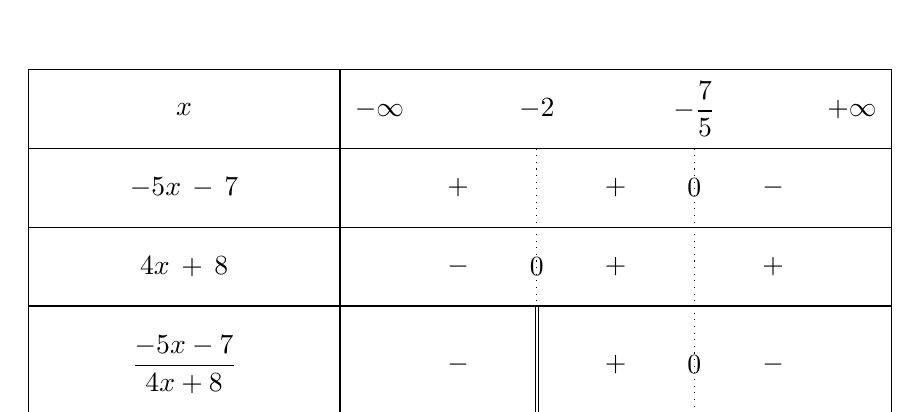
\begin{tikzpicture}
\tkzTabInit[lgt=3.96,espcl=2]{$x$ / 1, $- 5 x - 7$ / 1, $4 x + 8$ / 1, $\dfrac{- 5 x - 7}{4 x + 8}$ / 1.5}{$-\infty$, $-2$, $- \dfrac{7}{5}$, $+\infty$}
\tkzTabLine{, +, t, +, z, -}
\tkzTabLine{, -, z, +, t, +}
\tkzTabLine{, -, d, +, z, -}
\end{tikzpicture}
\end{center}
\par\smallskip
\begin{center}$S = \left] -\infty \,;\, -2 \right[ \cup \left[ - \dfrac{7}{5} \,;\, +\infty \right[$\end{center}\par\medskip
\noindent\textbf{2)}\par\smallskip
\begin{center}
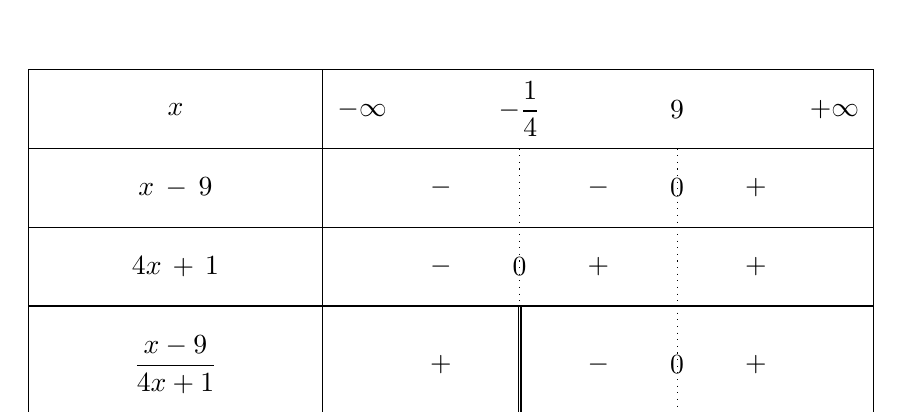
\begin{tikzpicture}
\tkzTabInit[lgt=3.74,espcl=2]{$x$ / 1, $x - 9$ / 1, $4 x + 1$ / 1, $\dfrac{x - 9}{4 x + 1}$ / 1.5}{$-\infty$, $- \dfrac{1}{4}$, $9$, $+\infty$}
\tkzTabLine{, -, t, -, z, +}
\tkzTabLine{, -, z, +, t, +}
\tkzTabLine{, +, d, -, z, +}
\end{tikzpicture}
\end{center}
\par\smallskip
\begin{center}$S = \left] -\infty \,;\, - \dfrac{1}{4} \right[ \cup \left] 9 \,;\, +\infty \right[$\end{center}\par\medskip
\noindent\textbf{3)}\par\smallskip
\begin{center}
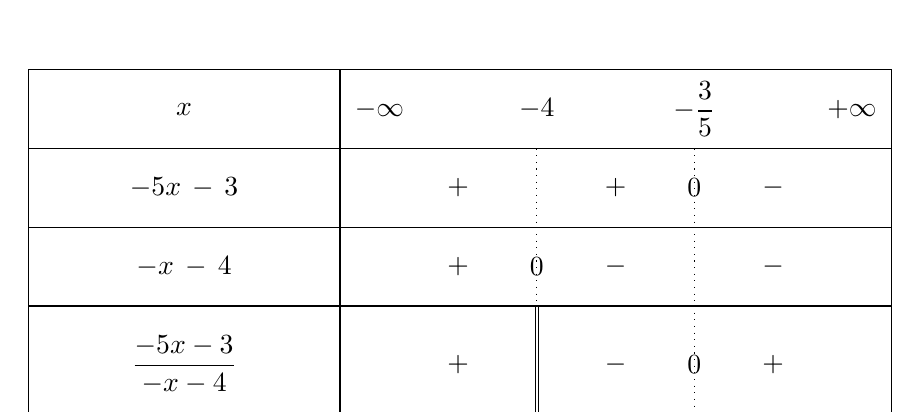
\begin{tikzpicture}
\tkzTabInit[lgt=3.96,espcl=2]{$x$ / 1, $- 5 x - 3$ / 1, $- x - 4$ / 1, $\dfrac{- 5 x - 3}{- x - 4}$ / 1.5}{$-\infty$, $-4$, $- \dfrac{3}{5}$, $+\infty$}
\tkzTabLine{, +, t, +, z, -}
\tkzTabLine{, +, z, -, t, -}
\tkzTabLine{, +, d, -, z, +}
\end{tikzpicture}
\end{center}
\par\smallskip
\begin{center}$S = \left] -4 \,;\, - \dfrac{3}{5} \right[$\end{center}\par\medskip
\noindent\textbf{4)}\par\smallskip
\begin{center}
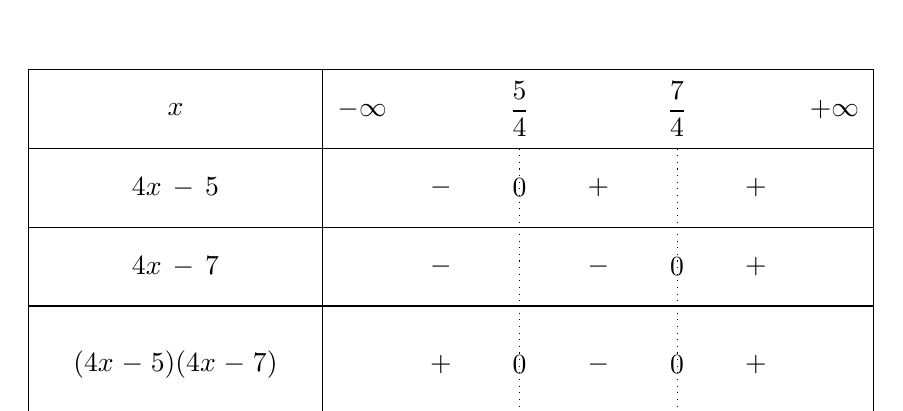
\begin{tikzpicture}
\tkzTabInit[lgt=3.74,espcl=2]{$x$ / 1, $4 x - 5$ / 1, $4 x - 7$ / 1, $(4 x - 5)(4 x - 7)$ / 1.5}{$-\infty$, $\dfrac{5}{4}$, $\dfrac{7}{4}$, $+\infty$}
\tkzTabLine{, -, z, +, t, +}
\tkzTabLine{, -, t, -, z, +}
\tkzTabLine{, +, z, -, z, +}
\end{tikzpicture}
\end{center}
\par\smallskip
\begin{center}$S = \left[ \dfrac{5}{4} \,;\, \dfrac{7}{4} \right]$\end{center}\par\medskip
\medskip

\noindent\textbf{Exercice 15}\par
\smallskip
\begin{enumerate}
\item $\dfrac{10^{-2} \times 10^{-1}}{10^{3}} = 10^{-6}$
\item $\dfrac{10^{-3} \times (10^{2})^{2}}{10^{4}} = 10^{-3}$
\item $\dfrac{10^{2} \times 10^{-2}}{10^{1}} = 10^{-1}$
\item $\dfrac{10^{0} \times (10^{3})^{2}}{10^{2}} = 10^{4}$
\end{enumerate}
\medskip

\noindent\textbf{Exercice 16}\par
\smallskip
\begin{enumerate}
\item $21 \sqrt{5}$
\item $42 \sqrt{5}$
\item $- 8 \sqrt{5} + 4 \sqrt{10}$
\item $- \sqrt{11} + 7 \sqrt{5}$
\item $- 33 \sqrt{5}$
\item $53 - 20 \sqrt{7}$
\end{enumerate}
\medskip

\noindent\textbf{Exercice 17}\par
\smallskip
\textbf{1)}
\begin{enumerate}
\item $\overrightarrow{\ensuremath{\mathrm{A}}\ensuremath{\mathrm{B}}}(1\,;\,2)$
\item $\overrightarrow{\ensuremath{\mathrm{A}}\ensuremath{\mathrm{B}}}(-4\,;\,-2)$
\item $\overrightarrow{\ensuremath{\mathrm{A}}\ensuremath{\mathrm{B}}}(7\,;\,-2)$
\end{enumerate}
\textbf{2)}
\begin{enumerate}
\item $\ensuremath{\mathrm{M}}\left(\dfrac{9}{2}\,;\,-3\right)$
\item $\ensuremath{\mathrm{M}}\left(1\,;\,-3\right)$
\end{enumerate}
\textbf{3)}
\begin{enumerate}
\item $\det(\vec{u},\vec{v}) = 2\times(-10)-(5)\times-4 = 0$. Oui.
\item $\det(\vec{u},\vec{v}) = 4\times(3)-(3)\times4 = 0$. Oui.
\end{enumerate}
\medskip

\noindent\textbf{Exercice 18}\par
\smallskip
\textbf{1)}
\begin{enumerate}
\item $m = \dfrac{-3-5}{-5--4} = 8$ donc $y = 8x + 37$
\item $m = \dfrac{-2--3}{5--5} = \dfrac{1}{10}$ donc $y = \dfrac{1}{10}x - \dfrac{5}{2}$
\item $m = \dfrac{2--2}{5--1} = \dfrac{2}{3}$ donc $y = \dfrac{2}{3}x - \dfrac{4}{3}$
\end{enumerate}
\textbf{2)}
\begin{enumerate}
\item On cherche les couples $(x\,;\,y)$ vérifiant les deux équations :

$4x + 1 = -x + 2$

$\Leftrightarrow 5x = 1$

$\Leftrightarrow x = \dfrac{1}{5}$

puis $y = 4 \times (\dfrac{1}{5}) + 1 = \dfrac{9}{5}$

Donc le point d'intersection est $\left(\dfrac{1}{5}\,;\,\dfrac{9}{5}\right)$.
\item On cherche les couples $(x\,;\,y)$ vérifiant les deux équations :

$-4x + 1 = -2x$

$\Leftrightarrow -2x = -1$

$\Leftrightarrow x = \dfrac{1}{2}$

puis $y = -4 \times (\dfrac{1}{2}) + 1 = -1$

Donc le point d'intersection est $\left(\dfrac{1}{2}\,;\,-1\right)$.
\end{enumerate}
\medskip

\newpage
\begin{center}
\textbf{Sujet numéro 3}
\\(à rendre avec la copie)
\end{center}


\noindent\textbf{Exercice 1} -- Développer les expressions suivantes.
\begin{enumerate}
\item $-8(8x - 7)$
\item $-8(5x - 2)$
\item $-8(5x + 5)$
\item $6(6x - 7)$
\end{enumerate}
\noindent\textbf{Exercice} -- Factoriser les expressions suivantes.
\begin{enumerate}
\item $-6x + 24$
\item $-21x + 28$
\item $30x - 35$
\item $-40x - 64$
\end{enumerate}
\bigskip

\noindent\textbf{Exercice 2} -- Calculer en respectant les priorités opératoires.
\begin{enumerate}
\item $(6 + 9) \times 5$
\item $9 \times (2 + 10) - 6$
\item $7 \times (8 + 5) + 5$
\item $7 \times (4 + 3) + 7$
\item $5 \times (5 + 4) - 4$
\item $(9 - 4) \times 4$
\end{enumerate}
\bigskip

\noindent\textbf{Exercice 3} -- Calculer les expressions suivantes.
\begin{enumerate}
\item $(+8) + (+6) + (-5)$
\item $(-3) + (-17) + (+1)$
\item $(-15) + (+9) + (+17)$
\item $(-18) + (-6) + (-17)$
\item $(+9) - (+9) + (+3)$
\item $(-15) + (+9) - (-16)$
\item $(-4) + (-19) - (-10)$
\item $(-10) - (-2) - (+14)$
\end{enumerate}
\bigskip

\noindent\textbf{Exercice 4} -- Développer et réduire.
\begin{enumerate}
\item $3x(7x - 5)$
\item $3x(-5x - 8)$
\item $(-6x - 7)(4x - 8)$
\item $(-2x - 7)(3x - 8)$
\item $(8 - 3x)(9x - 8)$
\item $(-7x - 9)(2x - 5)$
\end{enumerate}
\bigskip

\noindent\textbf{Exercice 5} -- Réduire les expressions suivantes.
\begin{enumerate}
\item $-(3 - 5x)-(5 - 4x)$
\item $(-4x - 6)-(6 - 6x)$
\item $-(3x - 8)+(7 - 7x)$
\item $(7x + 8)-(2 - 8x)$
\item $(-6x - 7)-(-5x - 9)$
\end{enumerate}
\bigskip

\noindent\textbf{Exercice 6} -- Théorème de Pythagore.
\medskip

\noindent\textbf{1.} Le triangle \ensuremath{\mathrm{A}}\ensuremath{\mathrm{B}}\ensuremath{\mathrm{C}} est rectangle en \ensuremath{\mathrm{B}}. On donne $\ensuremath{\mathrm{A}}\ensuremath{\mathrm{B}} = 8~\text{cm}$ et $\ensuremath{\mathrm{B}}\ensuremath{\mathrm{C}} = 15~\text{cm}$.

\begin{center}
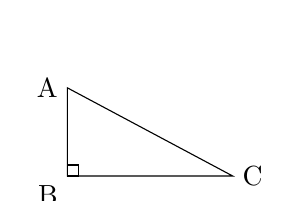
\begin{tikzpicture}[scale=0.35]
\draw (0,3.20) node[left]{A} -- (0,0) node[below left]{B} -- (6.00,0) node[right]{C} -- cycle;
\draw (0,0) rectangle (0.4,0.4);
\end{tikzpicture}
\end{center}

Calculer la valeur exacte de $\ensuremath{\mathrm{A}}\ensuremath{\mathrm{C}}$.

\medskip

\noindent\textbf{2.} Le triangle \ensuremath{\mathrm{D}}\ensuremath{\mathrm{E}}\ensuremath{\mathrm{F}} est rectangle en \ensuremath{\mathrm{E}}. On donne $\ensuremath{\mathrm{D}}\ensuremath{\mathrm{F}} = 30~\text{cm}$ et $\ensuremath{\mathrm{D}}\ensuremath{\mathrm{E}} = 18~\text{cm}$.

\begin{center}
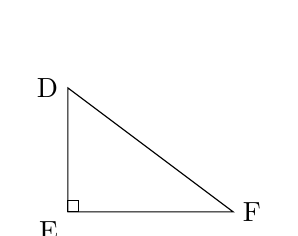
\begin{tikzpicture}[scale=0.35]
\draw (0,4.50) node[left]{D} -- (0,0) node[below left]{E} -- (6.00,0) node[right]{F} -- cycle;
\draw (0,0) rectangle (0.4,0.4);
\end{tikzpicture}
\end{center}

Calculer la valeur exacte de $\ensuremath{\mathrm{E}}\ensuremath{\mathrm{F}}$.

\medskip

\noindent\textbf{3.} Le triangle \ensuremath{\mathrm{M}}\ensuremath{\mathrm{N}}\ensuremath{\mathrm{P}} est rectangle en \ensuremath{\mathrm{N}}. On donne $\ensuremath{\mathrm{M}}\ensuremath{\mathrm{N}} = 5~\text{cm}$ et $\ensuremath{\mathrm{N}}\ensuremath{\mathrm{P}} = 7~\text{cm}$.

\begin{center}
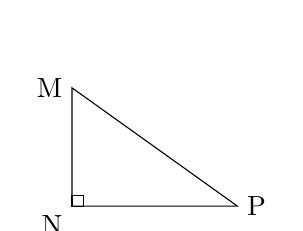
\begin{tikzpicture}[scale=0.35]
\draw (0,4.29) node[left]{M} -- (0,0) node[below left]{N} -- (6.00,0) node[right]{P} -- cycle;
\draw (0,0) rectangle (0.4,0.4);
\end{tikzpicture}
\end{center}

Calculer la valeur exacte de $\ensuremath{\mathrm{M}}\ensuremath{\mathrm{P}}$.

\medskip

\noindent\textbf{4.} Le triangle \ensuremath{\mathrm{R}}\ensuremath{\mathrm{S}}\ensuremath{\mathrm{T}} est rectangle en \ensuremath{\mathrm{S}}. On donne $\ensuremath{\mathrm{R}}\ensuremath{\mathrm{T}} = 8~\text{cm}$ et $\ensuremath{\mathrm{R}}\ensuremath{\mathrm{S}} = 6~\text{cm}$.

\begin{center}
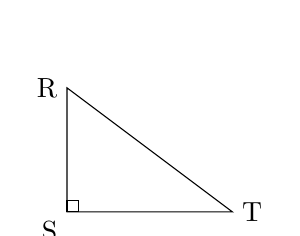
\begin{tikzpicture}[scale=0.35]
\draw (0,4.50) node[left]{R} -- (0,0) node[below left]{S} -- (6.00,0) node[right]{T} -- cycle;
\draw (0,0) rectangle (0.4,0.4);
\end{tikzpicture}
\end{center}

Calculer la valeur exacte de $\ensuremath{\mathrm{S}}\ensuremath{\mathrm{T}}$.

\medskip
\bigskip

\noindent\textbf{Exercice 7} -- Théorème de Thalès

\medskip
\noindent\textbf{1.} Les droites (\ensuremath{\mathrm{B}}\ensuremath{\mathrm{B}^\prime}) et (\ensuremath{\mathrm{C}}\ensuremath{\mathrm{C}^\prime}) sont parallèles. \ensuremath{\mathrm{A}}\ensuremath{\mathrm{B}} = 5, \ensuremath{\mathrm{A}}\ensuremath{\mathrm{C}} = 9, \ensuremath{\mathrm{A}}\ensuremath{\mathrm{B}^\prime} = 4.

\begin{center}
\begin{tikzpicture}[scale=0.8]
\draw [thick] (0.000,0.000)--(5.000,0.000);
\draw [thick] (5.000,0.000)--(9.000,0.000);
\draw [thick] (0.000,0.000)--(2.828,2.828);
\draw [thick] (2.828,2.828)--(5.091,5.091);
\draw [thick] (5.000,0.000)--(2.828,2.828);
\draw [thick] (9.000,0.000)--(5.091,5.091);
\draw (-0.400,-0.300) node {A};
\draw (5.000,-0.500) node {B};
\draw (9.000,-0.500) node {C};
\draw (2.428,3.128) node {B'};
\draw (5.391,5.391) node {C'};
\end{tikzpicture}
\end{center}
Déterminer en justifiant la valeur exacte de \ensuremath{\mathrm{A}}\ensuremath{\mathrm{C}^\prime}.

\bigskip
\noindent\textbf{2.} Les droites (\ensuremath{\mathrm{B}}\ensuremath{\mathrm{B}^\prime}) et (\ensuremath{\mathrm{C}}\ensuremath{\mathrm{C}^\prime}) sont parallèles. \ensuremath{\mathrm{A}}\ensuremath{\mathrm{B}^\prime} = 4, \ensuremath{\mathrm{A}}\ensuremath{\mathrm{B}} = 3, \ensuremath{\mathrm{A}}\ensuremath{\mathrm{C}} = 6.

\begin{center}
\begin{tikzpicture}[scale=0.8]
\draw [thick] (0.000,0.000)--(3.000,0.000);
\draw [thick] (3.000,0.000)--(6.000,0.000);
\draw [thick] (0.000,0.000)--(3.236,2.351);
\draw [thick] (3.236,2.351)--(6.472,4.702);
\draw [thick] (3.000,0.000)--(3.236,2.351);
\draw [thick] (6.000,0.000)--(6.472,4.702);
\draw (-0.400,-0.300) node {A};
\draw (3.000,-0.500) node {B};
\draw (6.000,-0.500) node {C};
\draw (2.836,2.651) node {B'};
\draw (6.772,5.002) node {C'};
\end{tikzpicture}
\end{center}
Déterminer en justifiant la valeur exacte de \ensuremath{\mathrm{A}}\ensuremath{\mathrm{C}^\prime}.

\bigskip
\noindent\textbf{3.} Les droites (\ensuremath{\mathrm{B}}\ensuremath{\mathrm{B}^\prime}) et (\ensuremath{\mathrm{C}}\ensuremath{\mathrm{C}^\prime}) sont parallèles. \ensuremath{\mathrm{A}}\ensuremath{\mathrm{B}} = 2, \ensuremath{\mathrm{A}}\ensuremath{\mathrm{C}} = 6, \ensuremath{\mathrm{A}}\ensuremath{\mathrm{B}^\prime} = 4.

\begin{center}
\begin{tikzpicture}[scale=0.8]
\draw [thick] (0.000,0.000)--(2.000,0.000);
\draw [thick] (2.000,0.000)--(-6.000,0.000);
\draw [thick] (0.000,0.000)--(3.236,2.351);
\draw [thick] (3.236,2.351)--(-9.708,-7.053);
\draw [thick] (2.000,0.000)--(3.236,2.351);
\draw [thick] (-6.000,0.000)--(-9.708,-7.053);
\draw (0.100,-0.500) node {A};
\draw (2.300,0.000) node {B};
\draw (-6.500,0.000) node {C};
\draw (3.536,2.551) node {B'};
\draw (-10.208,-7.253) node {C'};
\end{tikzpicture}
\end{center}
Déterminer en justifiant la valeur exacte de \ensuremath{\mathrm{A}}\ensuremath{\mathrm{C}^\prime}.

\bigskip
\noindent\textbf{4.} Les droites (\ensuremath{\mathrm{B}}\ensuremath{\mathrm{B}^\prime}) et (\ensuremath{\mathrm{C}}\ensuremath{\mathrm{C}^\prime}) sont parallèles. \ensuremath{\mathrm{A}}\ensuremath{\mathrm{B}} = 2, \ensuremath{\mathrm{A}}\ensuremath{\mathrm{C}} = 4, \ensuremath{\mathrm{A}}\ensuremath{\mathrm{B}^\prime} = 3.

\begin{center}
\begin{tikzpicture}[scale=0.8]
\draw [thick] (0.000,0.000)--(2.000,0.000);
\draw [thick] (2.000,0.000)--(-4.000,0.000);
\draw [thick] (0.000,0.000)--(2.121,2.121);
\draw [thick] (2.121,2.121)--(-4.243,-4.243);
\draw [thick] (2.000,0.000)--(2.121,2.121);
\draw [thick] (-4.000,0.000)--(-4.243,-4.243);
\draw (0.100,-0.500) node {A};
\draw (2.300,0.000) node {B};
\draw (-4.500,0.000) node {C};
\draw (2.421,2.321) node {B'};
\draw (-4.743,-4.443) node {C'};
\end{tikzpicture}
\end{center}
Déterminer en justifiant la valeur exacte de \ensuremath{\mathrm{A}}\ensuremath{\mathrm{C}^\prime}.
\bigskip

\noindent\textbf{Exercice 8} -- Résoudre les équations suivantes.
\begin{enumerate}
\item $-8x = -12$
\item $5x + 15 = 9$
\item $-6x - 7 = 8$
\item $9x + 11 = -3x - 2$
\item $3x - 11 = 5x + 6$
\end{enumerate}
\bigskip

\noindent\textbf{Exercice 9} -- Résoudre les équations suivantes.
\begin{enumerate}
\item $(9 - 2x)(-6x - 4) = 0$
\item $(-6x - 1)(x - 2) = 0$
\item $(-6x - 7)(3x + 4) = 0$
\item $(4 - 4x)(x + 7) = 0$
\end{enumerate}
\bigskip

\noindent\textbf{Exercice 10} -- Calculer et simplifier.
\begin{enumerate}
\item $\dfrac{10}{3} + \dfrac{4}{2}$
\item $\dfrac{7}{7} + \dfrac{6}{6}$
\item $\dfrac{1}{5} - \dfrac{1}{5} \times \dfrac{1}{5}$
\item $\dfrac{2}{3} - \dfrac{5}{3} \times \dfrac{2}{3}$
\item $\dfrac{4 + \dfrac{3}{2}}{\dfrac{3}{2} - \dfrac{3}{6}}$
\end{enumerate}
\bigskip

\noindent\textbf{Exercice 11} -- Factoriser les expressions suivantes.
\begin{enumerate}
\item $(5x + 7)(-2x - 5) - (5x + 7)(4 - 6x)$
\item $(x - 7)(-2x - 5) - (x - 7)(-6x - 5)$
\item $(3 - 3x)(-3x - 5) - (3 - 3x)(-6x - 5)$
\end{enumerate}
\bigskip

\noindent\textbf{Exercice 12} -- Factoriser en utilisant une identité remarquable.
\begin{enumerate}
\item $(x + 5)^2 - (4x - 1)^2$
\item $(x - 6)^2 - (4x + 1)^2$
\item $16x^2 - 64x + 64$
\end{enumerate}
\bigskip

\noindent\textbf{Exercice 13} -- Résoudre les inéquations suivantes.
\begin{enumerate}
\item $- 9 x \leq 3$
\item $8 x < 9$
\item $- 4 x - 3 \geq 8$
\item $7 x - 2 < -9$
\item $- 2 x - 7 < 8 x - 2$
\item $6 x - 9 \geq - 5 x - 3$
\end{enumerate}
\bigskip

\noindent\textbf{Exercice 14} -- Résoudre à l'aide d'un tableau de signes.
\begin{enumerate}
\item $\dfrac{3 x + 7}{5 x - 7} < 0$
\item $\left(1 - 5 x\right) \left(- x - 4\right) \leq 0$
\item $\dfrac{3 x + 9}{5 x + 1} \geq 0$
\item $\dfrac{3 x - 5}{4 x + 3} < 0$
\end{enumerate}
\bigskip

\noindent\textbf{Exercice 15} -- Écrire sous la forme d'une unique puissance de 10.
\begin{enumerate}
\item $\dfrac{10^{2} \times 10^{-1}}{10^{2}}$
\item $\dfrac{10^{-3} \times (10^{1})^{3}}{10^{1}}$
\item $\dfrac{10^{-2} \times 10^{-1}}{10^{2}}$
\item $\dfrac{10^{3} \times (10^{3})^{3}}{10^{4}}$
\end{enumerate}
\bigskip

\noindent\textbf{Exercice 16} -- Calculer et simplifier.
\begin{enumerate}
\item $\sqrt{3528}$
\item $\sqrt{108}$
\item $\sqrt{3} + 2\sqrt{10} + 5\sqrt{3} - \sqrt{10}$
\item $4\sqrt{7} - 5\sqrt{10} - 3\sqrt{7} - 4\sqrt{10}$
\item $\sqrt{20} + 5\sqrt{5} - 2\sqrt{180} - \sqrt{80}$
\item $(3 - 5\sqrt{10})^2$
\end{enumerate}
\bigskip

\noindent\textbf{Exercice 17} -- Vecteurs et coordonnées.\\
\medskip
\noindent\textbf{1)} Calculer les coordonnées de $\overrightarrow{\ensuremath{\mathrm{A}}\ensuremath{\mathrm{B}}}$.
\begin{enumerate}
\item $\ensuremath{\mathrm{A}}(5\,;\,1)$ et $\ensuremath{\mathrm{B}}(-1\,;\,0)$
\item $\ensuremath{\mathrm{A}}(-3\,;\,-5)$ et $\ensuremath{\mathrm{B}}(1\,;\,-4)$
\item $\ensuremath{\mathrm{A}}(0\,;\,-3)$ et $\ensuremath{\mathrm{B}}(3\,;\,-4)$
\end{enumerate}
\medskip
\noindent\textbf{2)} Calculer les coordonnées du milieu de $[\ensuremath{\mathrm{A}}\ensuremath{\mathrm{B}}]$.
\begin{enumerate}
\item $\ensuremath{\mathrm{A}}(-5\,;\,-6)$ et $\ensuremath{\mathrm{B}}(4\,;\,-1)$
\item $\ensuremath{\mathrm{A}}(-4\,;\,2)$ et $\ensuremath{\mathrm{B}}(7\,;\,-6)$
\end{enumerate}
\medskip
\noindent\textbf{3)} Les vecteurs $\vec{u}$ et $\vec{v}$ sont-ils colinéaires ?
\begin{enumerate}
\item $\vec{u}(-5\,;\,2)$ et $\vec{v}(-10\,;\,4)$
\item $\vec{u}(3\,;\,-3)$ et $\vec{v}(-3\,;\,5)$
\end{enumerate}
\bigskip

\noindent\textbf{Exercice 18} -- Équations de droites.
\medskip
\noindent\textbf{1)} Déterminer l'équation réduite de la droite $(\ensuremath{\mathrm{A}}\ensuremath{\mathrm{B}})$.
\begin{enumerate}
\item $\ensuremath{\mathrm{A}}(1\,;\,1)$ et $\ensuremath{\mathrm{B}}(-3\,;\,1)$
\item $\ensuremath{\mathrm{A}}(-2\,;\,-1)$ et $\ensuremath{\mathrm{B}}(3\,;\,3)$
\item $\ensuremath{\mathrm{A}}(5\,;\,3)$ et $\ensuremath{\mathrm{B}}(2\,;\,-1)$
\end{enumerate}
\noindent\textbf{2)} Déterminer le point d'intersection.
\begin{enumerate}
\item $(d_1): y = 2x + 3$ et $(d_2): y = 4x + 2$
\item $(d_1): y = -3x - 2$ et $(d_2): y = x - 1$
\end{enumerate}
\bigskip

\vfill
\begin{flushright}
\qrset{height=1.5cm}
\qrset{level=M}
\qrcode{Ex1: -64x + 56 | -40x + 16 | -40x - 40 | 36x - 42 | 3(-2x + 8) | 7(-3x + 4) | 5(6x - 7) | 8(-5x - 8)  //  Ex2: 75 | 102 | 96 | 56 | 41 | 20  //  Ex3: 9 | -19 | 11 | -41 | 3 | 10 | -13 | -22  //  Ex4: 21x^2 - 15x | -15x^2 - 24x | -24x^2 + 20x + 56 | -6x^2 - 5x + 56 | -27x^2 + 96x - 64 | -14x^2 + 17x + 45  //  Ex5: 9x - 8 | 2x - 12 | 15 - 10x | 15x + 6 | 2 - x  //  Ex6: sqrt(289)~ cm | sqrt(576)~ cm | sqrt(74)$ cm | sqrt(28)$ cm  //  Ex7: 36/5 | 8 | 12 | 6  //  Ex8: S = (3)/(2) | S = - (6)/(5) | S = - (5)/(2) | S = - (13)/(12) | S = - (17)/(2)  //  Ex9: S = - (2)/(3) ; (9)/(2) | S = - (1)/(6) ; 2 | S = - (4)/(3) ; - (7)/(6) | S = -7 ; 1  //  Ex10: (16)/(3) | 2 | (4)/(25) | - (4)/(9) | (11)/(2)  //  Ex11: (5x + 7)(4x - 9) | (x - 7)(4x) | (3 - 3x)(3x)  //  Ex12: -3(x - 2)(5x + 4) | -5(x - 1)(3x + 7) | (4x - 8)^2  //  Ex13: [ - (1)/(3) ; +inf [ | ] -inf ; (9)/(8) [ | ] -inf ; - (11)/(4) ] | ] -inf ; -1 [ | ] - (1)/(2) ; +inf [ | [ (6)/(11) ; +inf [  //  Ex14: ] - (7)/(3) ; (7)/(5) [ | [ -4 ; (1)/(5) ] | ] -inf ; -3 ] U ] - (1)/(5) ; +inf [ | ] - (3)/(4) ; (5)/(3) [  //  Ex15: 10^-1 | 10^-1 | 10^-5 | 10^8  //  Ex16: 42 sqrt(2) | 6 sqrt(3) | sqrt(10) + 6 sqrt(3) | - 9 sqrt(10) + sqrt(7) | - 9 sqrt(5) | 259 - 30 sqrt(10)  //  Ex17: AB(-6;-1) | AB(4;1) | AB(3;-1)  //  Ex18: y = 0x + 1 | y = (4)/(5)x + (3)/(5) | y = (4)/(3)x - (11)/(3)}
\end{flushright}
\newpage
\begin{center}
\textbf{Corrigé numéro 3}\\
\end{center}

\noindent\textbf{Exercice 1}\par
\smallskip
\begin{enumerate}
\item $-8(8x - 7) = -64x + 56$
\item $-8(5x - 2) = -40x + 16$
\item $-8(5x + 5) = -40x - 40$
\item $6(6x - 7) = 36x - 42$
\end{enumerate}
\begin{enumerate}
\item $-6x + 24 = 3(-2x + 8)$
\item $-21x + 28 = 7(-3x + 4)$
\item $30x - 35 = 5(6x - 7)$
\item $-40x - 64 = 8(-5x - 8)$
\end{enumerate}
\medskip

\noindent\textbf{Exercice 2}\par
\smallskip
\begin{enumerate}
\item $(6 + 9) \times 5$

$= 15 \times 5$

$= 75$
\item $9 \times (2 + 10) - 6$

$= 9 \times 12 - 6$

$= 108 - 6$

$= 102$
\item $7 \times (8 + 5) + 5$

$= 7 \times 13 + 5$

$= 91 + 5$

$= 96$
\item $7 \times (4 + 3) + 7$

$= 7 \times 7 + 7$

$= 49 + 7$

$= 56$
\item $5 \times (5 + 4) - 4$

$= 5 \times 9 - 4$

$= 45 - 4$

$= 41$
\item $(9 - 4) \times 4$

$= 5 \times 4$

$= 20$
\end{enumerate}
\medskip

\noindent\textbf{Exercice 3}\par
\smallskip
\begin{enumerate}
\item $(+8) + (+6) + (-5) = 9$
\item $(-3) + (-17) + (+1) = -19$
\item $(-15) + (+9) + (+17) = 11$
\item $(-18) + (-6) + (-17) = -41$
\item $(+9) - (+9) + (+3) = 3$
\item $(-15) + (+9) - (-16) = 10$
\item $(-4) + (-19) - (-10) = -13$
\item $(-10) - (-2) - (+14) = -22$
\end{enumerate}
\medskip

\noindent\textbf{Exercice 4}\par
\smallskip
\begin{enumerate}
\item $3x(7x - 5) = 21x^2 - 15x$
\item $3x(-5x - 8) = -15x^2 - 24x$
\item $(-6x - 7)(4x - 8) = -24x^2 + 20x + 56$
\item $(-2x - 7)(3x - 8) = -6x^2 - 5x + 56$
\item $(8 - 3x)(9x - 8) = -27x^2 + 96x - 64$
\item $(-7x - 9)(2x - 5) = -14x^2 + 17x + 45$
\end{enumerate}
\medskip

\noindent\textbf{Exercice 5}\par
\smallskip
\begin{enumerate}
\item $-(3 - 5x)-(5 - 4x) = 9x - 8$
\item $(-4x - 6)-(6 - 6x) = 2x - 12$
\item $-(3x - 8)+(7 - 7x) = 15 - 10x$
\item $(7x + 8)-(2 - 8x) = 15x + 6$
\item $(-6x - 7)-(-5x - 9) = 2 - x$
\end{enumerate}
\medskip

\noindent\textbf{Exercice 6}\par
\smallskip
\textbf{1.} D'après le théorème de Pythagore dans le triangle \ensuremath{\mathrm{A}}\ensuremath{\mathrm{B}}\ensuremath{\mathrm{C}} rectangle en \ensuremath{\mathrm{B}} :

$\ensuremath{\mathrm{A}}\ensuremath{\mathrm{C}}^2 = \ensuremath{\mathrm{A}}\ensuremath{\mathrm{B}}^2 + \ensuremath{\mathrm{B}}\ensuremath{\mathrm{C}}^2$

$\ensuremath{\mathrm{A}}\ensuremath{\mathrm{C}}^2 = (8~\text{cm})^2 + (15~\text{cm})^2 = 64~\text{cm}^2 + 225~\text{cm}^2 = 289~\text{cm}^2$

Donc $\ensuremath{\mathrm{A}}\ensuremath{\mathrm{C}} = \sqrt{289}~\text{cm} = 17~\text{cm}$

\medskip
\textbf{2.} D'après le théorème de Pythagore dans le triangle \ensuremath{\mathrm{D}}\ensuremath{\mathrm{E}}\ensuremath{\mathrm{F}} rectangle en \ensuremath{\mathrm{E}} :

$\ensuremath{\mathrm{D}}\ensuremath{\mathrm{F}}^2 = \ensuremath{\mathrm{D}}\ensuremath{\mathrm{E}}^2 + \ensuremath{\mathrm{E}}\ensuremath{\mathrm{F}}^2$

Donc $\ensuremath{\mathrm{E}}\ensuremath{\mathrm{F}}^2 = \ensuremath{\mathrm{D}}\ensuremath{\mathrm{F}}^2 - \ensuremath{\mathrm{D}}\ensuremath{\mathrm{E}}^2 = (30~\text{cm})^2 - (18~\text{cm})^2 = 900~\text{cm}^2 - 324~\text{cm}^2 = 576~\text{cm}^2$

Donc $\ensuremath{\mathrm{E}}\ensuremath{\mathrm{F}} = \sqrt{576}~\text{cm} = 24~\text{cm}$

\medskip
\textbf{3.} D'après le théorème de Pythagore :

$\ensuremath{\mathrm{M}}\ensuremath{\mathrm{P}}^2 = (5~\text{cm})^2 + (7~\text{cm})^2 = 25~\text{cm}^2 + 49~\text{cm}^2 = 74~\text{cm}^2$

Donc $\ensuremath{\mathrm{M}}\ensuremath{\mathrm{P}} = \sqrt{74}$ cm

\medskip
\textbf{4.} D'après le théorème de Pythagore :

$\ensuremath{\mathrm{R}}\ensuremath{\mathrm{T}}^2 = \ensuremath{\mathrm{R}}\ensuremath{\mathrm{S}}^2 + \ensuremath{\mathrm{S}}\ensuremath{\mathrm{T}}^2$

Donc $\ensuremath{\mathrm{S}}\ensuremath{\mathrm{T}}^2 = (8~\text{cm})^2 - (6~\text{cm})^2 = 64~\text{cm}^2 - 36~\text{cm}^2 = 28~\text{cm}^2$

Donc $\ensuremath{\mathrm{S}}\ensuremath{\mathrm{T}} = \sqrt{28}$ cm

\medskip
\medskip

\noindent\textbf{Exercice 7}\par
\smallskip
\textbf{1.} Comme (\ensuremath{\mathrm{B}}\ensuremath{\mathrm{B}^\prime}) et (\ensuremath{\mathrm{C}}\ensuremath{\mathrm{C}^\prime}) sont parallèles, d'après le théorème de Thalès : \[\dfrac{\ensuremath{\mathrm{A}}\ensuremath{\mathrm{C}^\prime}}{\ensuremath{\mathrm{A}}\ensuremath{\mathrm{C}}}=\dfrac{\ensuremath{\mathrm{A}}\ensuremath{\mathrm{B}^\prime}}{\ensuremath{\mathrm{A}}\ensuremath{\mathrm{B}}}=\dfrac{4}{5}.\]Donc \[\ensuremath{\mathrm{A}}\ensuremath{\mathrm{C}^\prime}=9\times\dfrac{4}{5}=\dfrac{36}{5}.\]\medskip
\textbf{2.} Comme (\ensuremath{\mathrm{B}}\ensuremath{\mathrm{B}^\prime}) et (\ensuremath{\mathrm{C}}\ensuremath{\mathrm{C}^\prime}) sont parallèles, d'après le théorème de Thalès : \[\dfrac{\ensuremath{\mathrm{A}}\ensuremath{\mathrm{C}^\prime}}{\ensuremath{\mathrm{A}}\ensuremath{\mathrm{C}}}=\dfrac{\ensuremath{\mathrm{A}}\ensuremath{\mathrm{B}^\prime}}{\ensuremath{\mathrm{A}}\ensuremath{\mathrm{B}}}=\dfrac{4}{3}.\]Donc \[\ensuremath{\mathrm{A}}\ensuremath{\mathrm{C}^\prime}=6\times\dfrac{4}{3}=8.\]\medskip
\textbf{3.} Comme (\ensuremath{\mathrm{B}}\ensuremath{\mathrm{B}^\prime}) et (\ensuremath{\mathrm{C}}\ensuremath{\mathrm{C}^\prime}) sont parallèles, d'après le théorème de Thalès : \[\dfrac{\ensuremath{\mathrm{A}}\ensuremath{\mathrm{C}^\prime}}{\ensuremath{\mathrm{A}}\ensuremath{\mathrm{C}}}=\dfrac{\ensuremath{\mathrm{A}}\ensuremath{\mathrm{B}^\prime}}{\ensuremath{\mathrm{A}}\ensuremath{\mathrm{B}}}=\dfrac{4}{2}.\]Donc \[\ensuremath{\mathrm{A}}\ensuremath{\mathrm{C}^\prime}=6\times\dfrac{4}{2}=12.\]\medskip
\textbf{4.} Comme (\ensuremath{\mathrm{B}}\ensuremath{\mathrm{B}^\prime}) et (\ensuremath{\mathrm{C}}\ensuremath{\mathrm{C}^\prime}) sont parallèles, d'après le théorème de Thalès : \[\dfrac{\ensuremath{\mathrm{A}}\ensuremath{\mathrm{C}^\prime}}{\ensuremath{\mathrm{A}}\ensuremath{\mathrm{C}}}=\dfrac{\ensuremath{\mathrm{A}}\ensuremath{\mathrm{B}^\prime}}{\ensuremath{\mathrm{A}}\ensuremath{\mathrm{B}}}=\dfrac{3}{2}.\]Donc \[\ensuremath{\mathrm{A}}\ensuremath{\mathrm{C}^\prime}=4\times\dfrac{3}{2}=6.\]\medskip
\medskip

\noindent\textbf{Exercice 8}\par
\smallskip
\begin{enumerate}
\item $-8x = -12$

$\Leftrightarrow x = \dfrac{-12}{-8} = \dfrac{3}{2}$

L'ensemble des solutions est $S = \left\{\dfrac{3}{2}\right\}$.

\item $5x + 15 = 9$

$\Leftrightarrow 5x = 9 - (15) = -6$

$\Leftrightarrow x = \dfrac{-6}{5} = - \dfrac{6}{5}$

L'ensemble des solutions est $S = \left\{- \dfrac{6}{5}\right\}$.

\item $-6x - 7 = 8$

$\Leftrightarrow -6x = 8 - (-7) = 15$

$\Leftrightarrow x = \dfrac{15}{-6} = - \dfrac{5}{2}$

L'ensemble des solutions est $S = \left\{- \dfrac{5}{2}\right\}$.

\item $9x + 11 = -3x - 2$

$\Leftrightarrow 12x = -13$

$\Leftrightarrow x = \dfrac{-13}{12} = - \dfrac{13}{12}$

L'ensemble des solutions est $S = \left\{- \dfrac{13}{12}\right\}$.

\item $3x - 11 = 5x + 6$

$\Leftrightarrow -2x = 17$

$\Leftrightarrow x = \dfrac{17}{-2} = - \dfrac{17}{2}$

L'ensemble des solutions est $S = \left\{- \dfrac{17}{2}\right\}$.

\end{enumerate}
\medskip

\noindent\textbf{Exercice 9}\par
\smallskip
\begin{enumerate}
\item Un produit est nul si et seulement si l'un des facteurs est nul.

$\bullet\ -6x - 4 = 0 \Leftrightarrow x = - \dfrac{2}{3}$

$\bullet\ 9 - 2x = 0 \Leftrightarrow x = \dfrac{9}{2}$

Donc $S = \left\{- \dfrac{2}{3} \; ; \; \dfrac{9}{2}\right\}$

\item Un produit est nul si et seulement si l'un des facteurs est nul.

$\bullet\ x - 2 = 0 \Leftrightarrow x = 2$

$\bullet\ -6x - 1 = 0 \Leftrightarrow x = - \dfrac{1}{6}$

Donc $S = \left\{- \dfrac{1}{6} \; ; \; 2\right\}$

\item Un produit est nul si et seulement si l'un des facteurs est nul.

$\bullet\ -6x - 7 = 0 \Leftrightarrow x = - \dfrac{7}{6}$

$\bullet\ 3x + 4 = 0 \Leftrightarrow x = - \dfrac{4}{3}$

Donc $S = \left\{- \dfrac{4}{3} \; ; \; - \dfrac{7}{6}\right\}$

\item Un produit est nul si et seulement si l'un des facteurs est nul.

$\bullet\ 4 - 4x = 0 \Leftrightarrow x = 1$

$\bullet\ x + 7 = 0 \Leftrightarrow x = -7$

Donc $S = \left\{-7 \; ; \; 1\right\}$

\end{enumerate}
\medskip

\noindent\textbf{Exercice 10}\par
\smallskip
\begin{enumerate}
\item $\dfrac{10 \times 2}{3 \times 2} + \dfrac{4 \times 3}{2 \times 3} = \dfrac{32}{6} = \dfrac{16}{3}$
\item $\dfrac{7 \times 6}{7 \times 6} + \dfrac{6 \times 7}{6 \times 7} = \dfrac{84}{42} = 2$
\item $= \dfrac{1}{5} - \dfrac{1}{25}$ (priorité $\times$)

$= \dfrac{5}{25} - \dfrac{1}{25} = \dfrac{4}{25}$
\item $= \dfrac{2}{3} - \dfrac{10}{9}$ (priorité $\times$)

$= \dfrac{6}{9} - \dfrac{10}{9} = \dfrac{-4}{9}$
\item Numérateur : $4 + \dfrac{3}{2} = \dfrac{4 \times 2 + 3}{2} = \dfrac{11}{2}$

Dénominateur : $\dfrac{3}{2} - \dfrac{3}{6} = \dfrac{3 \times 6 - 3 \times 2}{2 \times 6} = 1$

$= \dfrac{11}{2} \div 1 = \dfrac{11}{2} \times 1 = \dfrac{11}{2}$
\end{enumerate}
\medskip

\noindent\textbf{Exercice 11}\par
\smallskip
\begin{enumerate}
\item $(5x + 7)(4x - 9)$
\item $(x - 7)(4x)$
\item $(3 - 3x)(3x)$
\end{enumerate}
\medskip

\noindent\textbf{Exercice 12}\par
\smallskip
\begin{enumerate}
\item $-3(x - 2)(5x + 4)$
\item $-5(x - 1)(3x + 7)$
\item $(4x - 8)^2$
\end{enumerate}
\medskip

\noindent\textbf{Exercice 13}\par
\smallskip
\begin{enumerate}
\item $-9x \leq 3$

$\Leftrightarrow x \geq - \dfrac{1}{3}$

$S = \left[ - \dfrac{1}{3} \,;\, +\infty \right[$
\item $8x < 9$

$\Leftrightarrow x < \dfrac{9}{8}$

$S = \left] -\infty \,;\, \dfrac{9}{8} \right[$
\item $- 4 x - 3 \geq 8$

$\Leftrightarrow -4x \geq 8 - (-3) = 11$

$\Leftrightarrow x \leq - \dfrac{11}{4}$

$S = \left] -\infty \,;\, - \dfrac{11}{4} \right]$
\item $7 x - 2 < -9$

$\Leftrightarrow 7x < -9 - (-2) = -7$

$\Leftrightarrow x < -1$

$S = \left] -\infty \,;\, -1 \right[$
\item $- 2 x - 7 < 8 x - 2$

$\Leftrightarrow -10x < 5$

$\Leftrightarrow x > - \dfrac{1}{2}$

$S = \left] - \dfrac{1}{2} \,;\, +\infty \right[$
\item $6 x - 9 \geq - 5 x - 3$

$\Leftrightarrow 11x \geq 6$

$\Leftrightarrow x \geq \dfrac{6}{11}$

$S = \left[ \dfrac{6}{11} \,;\, +\infty \right[$
\end{enumerate}
\medskip

\noindent\textbf{Exercice 14}\par
\smallskip
\noindent\textbf{1)}\par\smallskip
\begin{center}
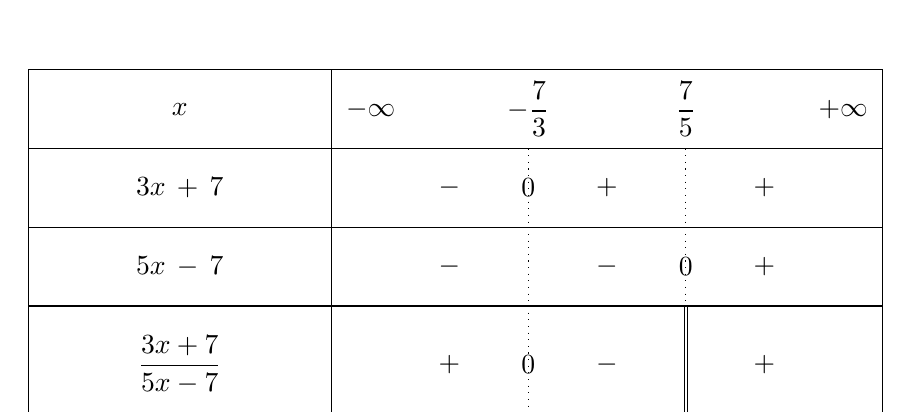
\begin{tikzpicture}
\tkzTabInit[lgt=3.85,espcl=2]{$x$ / 1, $3 x + 7$ / 1, $5 x - 7$ / 1, $\dfrac{3 x + 7}{5 x - 7}$ / 1.5}{$-\infty$, $- \dfrac{7}{3}$, $\dfrac{7}{5}$, $+\infty$}
\tkzTabLine{, -, z, +, t, +}
\tkzTabLine{, -, t, -, z, +}
\tkzTabLine{, +, z, -, d, +}
\end{tikzpicture}
\end{center}
\par\smallskip
\begin{center}$S = \left] - \dfrac{7}{3} \,;\, \dfrac{7}{5} \right[$\end{center}\par\medskip
\noindent\textbf{2)}\par\smallskip
\begin{center}
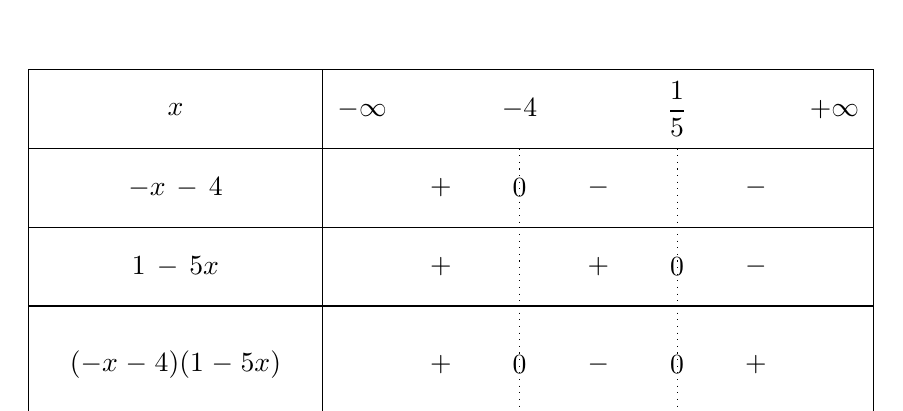
\begin{tikzpicture}
\tkzTabInit[lgt=3.74,espcl=2]{$x$ / 1, $- x - 4$ / 1, $1 - 5 x$ / 1, $(- x - 4)(1 - 5 x)$ / 1.5}{$-\infty$, $-4$, $\dfrac{1}{5}$, $+\infty$}
\tkzTabLine{, +, z, -, t, -}
\tkzTabLine{, +, t, +, z, -}
\tkzTabLine{, +, z, -, z, +}
\end{tikzpicture}
\end{center}
\par\smallskip
\begin{center}$S = \left[ -4 \,;\, \dfrac{1}{5} \right]$\end{center}\par\medskip
\noindent\textbf{3)}\par\smallskip
\begin{center}
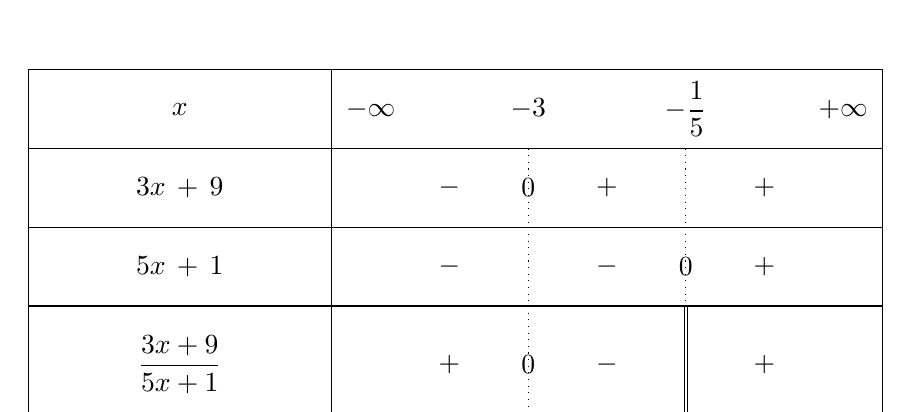
\begin{tikzpicture}
\tkzTabInit[lgt=3.85,espcl=2]{$x$ / 1, $3 x + 9$ / 1, $5 x + 1$ / 1, $\dfrac{3 x + 9}{5 x + 1}$ / 1.5}{$-\infty$, $-3$, $- \dfrac{1}{5}$, $+\infty$}
\tkzTabLine{, -, z, +, t, +}
\tkzTabLine{, -, t, -, z, +}
\tkzTabLine{, +, z, -, d, +}
\end{tikzpicture}
\end{center}
\par\smallskip
\begin{center}$S = \left] -\infty \,;\, -3 \right] \cup \left] - \dfrac{1}{5} \,;\, +\infty \right[$\end{center}\par\medskip
\noindent\textbf{4)}\par\smallskip
\begin{center}
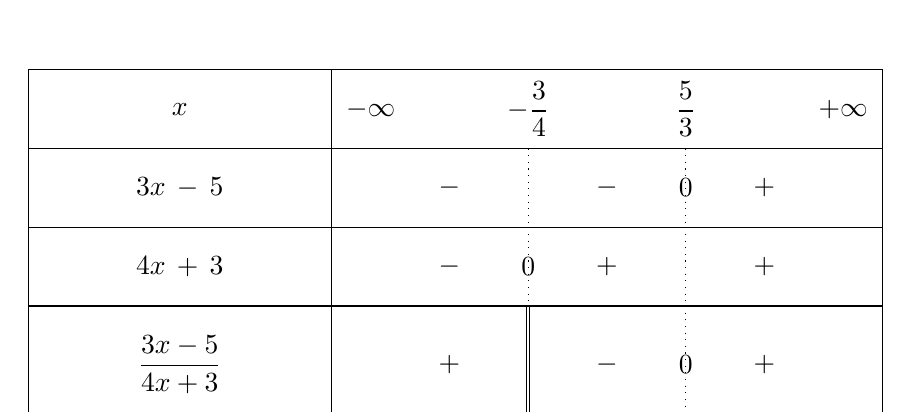
\begin{tikzpicture}
\tkzTabInit[lgt=3.85,espcl=2]{$x$ / 1, $3 x - 5$ / 1, $4 x + 3$ / 1, $\dfrac{3 x - 5}{4 x + 3}$ / 1.5}{$-\infty$, $- \dfrac{3}{4}$, $\dfrac{5}{3}$, $+\infty$}
\tkzTabLine{, -, t, -, z, +}
\tkzTabLine{, -, z, +, t, +}
\tkzTabLine{, +, d, -, z, +}
\end{tikzpicture}
\end{center}
\par\smallskip
\begin{center}$S = \left] - \dfrac{3}{4} \,;\, \dfrac{5}{3} \right[$\end{center}\par\medskip
\medskip

\noindent\textbf{Exercice 15}\par
\smallskip
\begin{enumerate}
\item $\dfrac{10^{2} \times 10^{-1}}{10^{2}} = 10^{-1}$
\item $\dfrac{10^{-3} \times (10^{1})^{3}}{10^{1}} = 10^{-1}$
\item $\dfrac{10^{-2} \times 10^{-1}}{10^{2}} = 10^{-5}$
\item $\dfrac{10^{3} \times (10^{3})^{3}}{10^{4}} = 10^{8}$
\end{enumerate}
\medskip

\noindent\textbf{Exercice 16}\par
\smallskip
\begin{enumerate}
\item $42 \sqrt{2}$
\item $6 \sqrt{3}$
\item $\sqrt{10} + 6 \sqrt{3}$
\item $- 9 \sqrt{10} + \sqrt{7}$
\item $- 9 \sqrt{5}$
\item $259 - 30 \sqrt{10}$
\end{enumerate}
\medskip

\noindent\textbf{Exercice 17}\par
\smallskip
\textbf{1)}
\begin{enumerate}
\item $\overrightarrow{\ensuremath{\mathrm{A}}\ensuremath{\mathrm{B}}}(-6\,;\,-1)$
\item $\overrightarrow{\ensuremath{\mathrm{A}}\ensuremath{\mathrm{B}}}(4\,;\,1)$
\item $\overrightarrow{\ensuremath{\mathrm{A}}\ensuremath{\mathrm{B}}}(3\,;\,-1)$
\end{enumerate}
\textbf{2)}
\begin{enumerate}
\item $\ensuremath{\mathrm{M}}\left(- \dfrac{1}{2}\,;\,- \dfrac{7}{2}\right)$
\item $\ensuremath{\mathrm{M}}\left(\dfrac{3}{2}\,;\,-2\right)$
\end{enumerate}
\textbf{3)}
\begin{enumerate}
\item $\det(\vec{u},\vec{v}) = -5\times(4)-(2)\times-10 = 0$. Oui.
\item $\det(\vec{u},\vec{v}) = 3\times(5)-(-3)\times-3 = 6$. Non.
\end{enumerate}
\medskip

\noindent\textbf{Exercice 18}\par
\smallskip
\textbf{1)}
\begin{enumerate}
\item $m = \dfrac{1-1}{-3-1} = 0$ donc $y = 0x + 1$
\item $m = \dfrac{3--1}{3--2} = \dfrac{4}{5}$ donc $y = \dfrac{4}{5}x + \dfrac{3}{5}$
\item $m = \dfrac{-1-3}{2-5} = \dfrac{4}{3}$ donc $y = \dfrac{4}{3}x - \dfrac{11}{3}$
\end{enumerate}
\textbf{2)}
\begin{enumerate}
\item On cherche les couples $(x\,;\,y)$ vérifiant les deux équations :

$2x + 3 = 4x + 2$

$\Leftrightarrow -2x = -1$

$\Leftrightarrow x = \dfrac{1}{2}$

puis $y = 2 \times (\dfrac{1}{2}) + 3 = 4$

Donc le point d'intersection est $\left(\dfrac{1}{2}\,;\,4\right)$.
\item On cherche les couples $(x\,;\,y)$ vérifiant les deux équations :

$-3x - 2 = x - 1$

$\Leftrightarrow -4x = 1$

$\Leftrightarrow x = - \dfrac{1}{4}$

puis $y = -3 \times (- \dfrac{1}{4}) - 2 = - \dfrac{5}{4}$

Donc le point d'intersection est $\left(- \dfrac{1}{4}\,;\,- \dfrac{5}{4}\right)$.
\end{enumerate}
\medskip

\newpage
\begin{center}
\textbf{Sujet numéro 4}
\\(à rendre avec la copie)
\end{center}


\noindent\textbf{Exercice 1} -- Développer les expressions suivantes.
\begin{enumerate}
\item $6(-x + 8)$
\item $-9(8x - 6)$
\item $-6(-5x - 3)$
\item $3(-2x + 5)$
\end{enumerate}
\noindent\textbf{Exercice} -- Factoriser les expressions suivantes.
\begin{enumerate}
\item $9x + 27$
\item $-24x - 28$
\item $42x + 63$
\item $-27x + 36$
\end{enumerate}
\bigskip

\noindent\textbf{Exercice 2} -- Calculer en respectant les priorités opératoires.
\begin{enumerate}
\item $3 \times (7 + 10) + 2$
\item $(10 + 8) \times 6$
\item $7 \times (9 - 9) + 2$
\item $5 \times (4 - 6) + 8$
\item $3 \times (4 + 8) - 9$
\item $(11 + 4) \times 4$
\end{enumerate}
\bigskip

\noindent\textbf{Exercice 3} -- Calculer les expressions suivantes.
\begin{enumerate}
\item $(-5) + (-7) + (-9)$
\item $(-1) + (-4) + (-17)$
\item $(-9) + (+12) + (-6)$
\item $(+16) + (-18) + (+4)$
\item $(+11) + (-19) - (-4)$
\item $(-7) + (-16) - (+17)$
\item $(+10) + (-16) - (-11)$
\item $(-17) + (+16) - (+14)$
\end{enumerate}
\bigskip

\noindent\textbf{Exercice 4} -- Développer et réduire.
\begin{enumerate}
\item $-9x(9x - 8)$
\item $-9x(2x - 5)$
\item $(4 - 6x)(6x + 7)$
\item $(7 - 3x)(-3x - 8)$
\item $(5 - 6x)(4x + 4)$
\item $(-6x - 3)(-2x - 4)$
\end{enumerate}
\bigskip

\noindent\textbf{Exercice 5} -- Réduire les expressions suivantes.
\begin{enumerate}
\item $(9x + 2)+(5 - 2x)$
\item $-(2x + 6)-(4x + 5)$
\item $-(-2x - 8)+(4x + 5)$
\item $-(8x - 8)-(9x - 9)$
\item $-(8x - 7)-(4x + 5)$
\end{enumerate}
\bigskip

\noindent\textbf{Exercice 6} -- Théorème de Pythagore.
\medskip

\noindent\textbf{1.} Le triangle \ensuremath{\mathrm{A}}\ensuremath{\mathrm{B}}\ensuremath{\mathrm{C}} est rectangle en \ensuremath{\mathrm{B}}. On donne $\ensuremath{\mathrm{A}}\ensuremath{\mathrm{B}} = 7~\text{cm}$ et $\ensuremath{\mathrm{B}}\ensuremath{\mathrm{C}} = 24~\text{cm}$.

\begin{center}
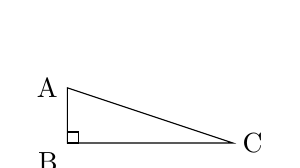
\begin{tikzpicture}[scale=0.35]
\draw (0,2.00) node[left]{A} -- (0,0) node[below left]{B} -- (6.00,0) node[right]{C} -- cycle;
\draw (0,0) rectangle (0.4,0.4);
\end{tikzpicture}
\end{center}

Calculer la valeur exacte de $\ensuremath{\mathrm{A}}\ensuremath{\mathrm{C}}$.

\medskip

\noindent\textbf{2.} Le triangle \ensuremath{\mathrm{D}}\ensuremath{\mathrm{E}}\ensuremath{\mathrm{F}} est rectangle en \ensuremath{\mathrm{E}}. On donne $\ensuremath{\mathrm{D}}\ensuremath{\mathrm{F}} = 75~\text{cm}$ et $\ensuremath{\mathrm{D}}\ensuremath{\mathrm{E}} = 21~\text{cm}$.

\begin{center}
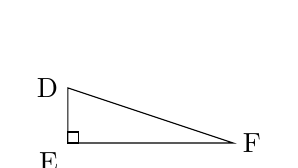
\begin{tikzpicture}[scale=0.35]
\draw (0,2.00) node[left]{D} -- (0,0) node[below left]{E} -- (6.00,0) node[right]{F} -- cycle;
\draw (0,0) rectangle (0.4,0.4);
\end{tikzpicture}
\end{center}

Calculer la valeur exacte de $\ensuremath{\mathrm{E}}\ensuremath{\mathrm{F}}$.

\medskip

\noindent\textbf{3.} Le triangle \ensuremath{\mathrm{M}}\ensuremath{\mathrm{N}}\ensuremath{\mathrm{P}} est rectangle en \ensuremath{\mathrm{N}}. On donne $\ensuremath{\mathrm{M}}\ensuremath{\mathrm{N}} = 7~\text{cm}$ et $\ensuremath{\mathrm{N}}\ensuremath{\mathrm{P}} = 11~\text{cm}$.

\begin{center}
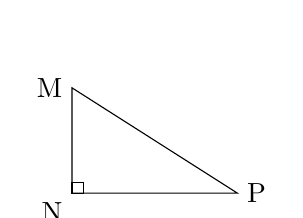
\begin{tikzpicture}[scale=0.35]
\draw (0,3.82) node[left]{M} -- (0,0) node[below left]{N} -- (6.00,0) node[right]{P} -- cycle;
\draw (0,0) rectangle (0.4,0.4);
\end{tikzpicture}
\end{center}

Calculer la valeur exacte de $\ensuremath{\mathrm{M}}\ensuremath{\mathrm{P}}$.

\medskip

\noindent\textbf{4.} Le triangle \ensuremath{\mathrm{R}}\ensuremath{\mathrm{S}}\ensuremath{\mathrm{T}} est rectangle en \ensuremath{\mathrm{S}}. On donne $\ensuremath{\mathrm{R}}\ensuremath{\mathrm{T}} = 11~\text{cm}$ et $\ensuremath{\mathrm{R}}\ensuremath{\mathrm{S}} = 5~\text{cm}$.

\begin{center}
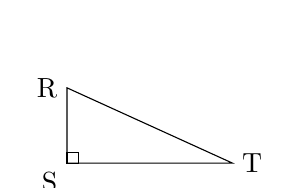
\begin{tikzpicture}[scale=0.35]
\draw (0,2.73) node[left]{R} -- (0,0) node[below left]{S} -- (6.00,0) node[right]{T} -- cycle;
\draw (0,0) rectangle (0.4,0.4);
\end{tikzpicture}
\end{center}

Calculer la valeur exacte de $\ensuremath{\mathrm{S}}\ensuremath{\mathrm{T}}$.

\medskip
\bigskip

\noindent\textbf{Exercice 7} -- Théorème de Thalès

\medskip
\noindent\textbf{1.} Les droites (\ensuremath{\mathrm{B}}\ensuremath{\mathrm{B}^\prime}) et (\ensuremath{\mathrm{C}}\ensuremath{\mathrm{C}^\prime}) sont parallèles. \ensuremath{\mathrm{A}}\ensuremath{\mathrm{C}} = 6, \ensuremath{\mathrm{A}}\ensuremath{\mathrm{B}^\prime} = 4, \ensuremath{\mathrm{A}}\ensuremath{\mathrm{B}} = 3.

\begin{center}
\begin{tikzpicture}[scale=0.8]
\draw [thick] (0.000,0.000)--(3.000,0.000);
\draw [thick] (3.000,0.000)--(6.000,0.000);
\draw [thick] (0.000,0.000)--(2.828,2.828);
\draw [thick] (2.828,2.828)--(5.657,5.657);
\draw [thick] (3.000,0.000)--(2.828,2.828);
\draw [thick] (6.000,0.000)--(5.657,5.657);
\draw (-0.400,-0.300) node {A};
\draw (3.000,-0.500) node {B};
\draw (6.000,-0.500) node {C};
\draw (2.428,3.128) node {B'};
\draw (5.957,5.957) node {C'};
\end{tikzpicture}
\end{center}
Déterminer en justifiant la valeur exacte de \ensuremath{\mathrm{A}}\ensuremath{\mathrm{C}^\prime}.

\bigskip
\noindent\textbf{2.} Les droites (\ensuremath{\mathrm{B}}\ensuremath{\mathrm{B}^\prime}) et (\ensuremath{\mathrm{C}}\ensuremath{\mathrm{C}^\prime}) sont parallèles. \ensuremath{\mathrm{A}}\ensuremath{\mathrm{B}^\prime} = 3, \ensuremath{\mathrm{A}}\ensuremath{\mathrm{B}} = 5, \ensuremath{\mathrm{A}}\ensuremath{\mathrm{C}} = 9.

\begin{center}
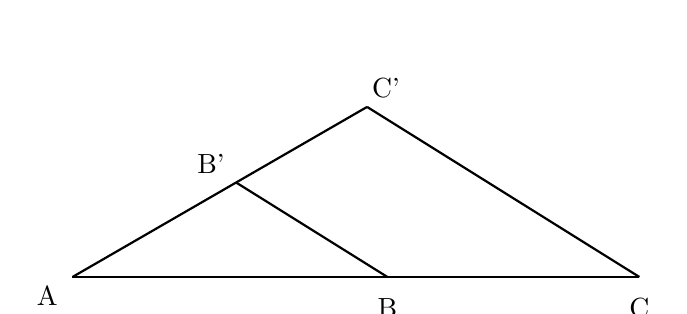
\begin{tikzpicture}[scale=0.8]
\draw [thick] (0.000,0.000)--(5.000,0.000);
\draw [thick] (5.000,0.000)--(9.000,0.000);
\draw [thick] (0.000,0.000)--(2.598,1.500);
\draw [thick] (2.598,1.500)--(4.677,2.700);
\draw [thick] (5.000,0.000)--(2.598,1.500);
\draw [thick] (9.000,0.000)--(4.677,2.700);
\draw (-0.400,-0.300) node {A};
\draw (5.000,-0.500) node {B};
\draw (9.000,-0.500) node {C};
\draw (2.198,1.800) node {B'};
\draw (4.977,3.000) node {C'};
\end{tikzpicture}
\end{center}
Déterminer en justifiant la valeur exacte de \ensuremath{\mathrm{A}}\ensuremath{\mathrm{C}^\prime}.

\bigskip
\noindent\textbf{3.} Les droites (\ensuremath{\mathrm{B}}\ensuremath{\mathrm{B}^\prime}) et (\ensuremath{\mathrm{C}}\ensuremath{\mathrm{C}^\prime}) sont parallèles. \ensuremath{\mathrm{A}}\ensuremath{\mathrm{B}^\prime} = 4, \ensuremath{\mathrm{A}}\ensuremath{\mathrm{C}} = 6, \ensuremath{\mathrm{A}}\ensuremath{\mathrm{B}} = 2.

\begin{center}
\begin{tikzpicture}[scale=0.8]
\draw [thick] (0.000,0.000)--(2.000,0.000);
\draw [thick] (2.000,0.000)--(-6.000,0.000);
\draw [thick] (0.000,0.000)--(2.828,2.828);
\draw [thick] (2.828,2.828)--(-8.485,-8.485);
\draw [thick] (2.000,0.000)--(2.828,2.828);
\draw [thick] (-6.000,0.000)--(-8.485,-8.485);
\draw (0.100,-0.500) node {A};
\draw (2.300,0.000) node {B};
\draw (-6.500,0.000) node {C};
\draw (3.128,3.028) node {B'};
\draw (-8.985,-8.685) node {C'};
\end{tikzpicture}
\end{center}
Déterminer en justifiant la valeur exacte de \ensuremath{\mathrm{A}}\ensuremath{\mathrm{C}^\prime}.

\bigskip
\noindent\textbf{4.} Les droites (\ensuremath{\mathrm{B}}\ensuremath{\mathrm{B}^\prime}) et (\ensuremath{\mathrm{C}}\ensuremath{\mathrm{C}^\prime}) sont parallèles. \ensuremath{\mathrm{A}}\ensuremath{\mathrm{C}} = 5, \ensuremath{\mathrm{A}}\ensuremath{\mathrm{B}} = 2, \ensuremath{\mathrm{A}}\ensuremath{\mathrm{B}^\prime} = 3.

\begin{center}
\begin{tikzpicture}[scale=0.8]
\draw [thick] (0.000,0.000)--(2.000,0.000);
\draw [thick] (2.000,0.000)--(-5.000,0.000);
\draw [thick] (0.000,0.000)--(2.598,1.500);
\draw [thick] (2.598,1.500)--(-6.495,-3.750);
\draw [thick] (2.000,0.000)--(2.598,1.500);
\draw [thick] (-5.000,0.000)--(-6.495,-3.750);
\draw (0.100,-0.500) node {A};
\draw (2.300,0.000) node {B};
\draw (-5.500,0.000) node {C};
\draw (2.898,1.700) node {B'};
\draw (-6.995,-3.950) node {C'};
\end{tikzpicture}
\end{center}
Déterminer en justifiant la valeur exacte de \ensuremath{\mathrm{A}}\ensuremath{\mathrm{C}^\prime}.
\bigskip

\noindent\textbf{Exercice 8} -- Résoudre les équations suivantes.
\begin{enumerate}
\item $8x = -20$
\item $6x + 7 = 5$
\item $9 - 3x = 3$
\item $10 - 2x = 1 - 5x$
\item $-6x - 4 = 4 - 5x$
\end{enumerate}
\bigskip

\noindent\textbf{Exercice 9} -- Résoudre les équations suivantes.
\begin{enumerate}
\item $(6 - 7x)(-2x - 1) = 0$
\item $(-x - 1)(2x - 7) = 0$
\item $(-2x - 2)(6x - 4) = 0$
\item $(-3x - 6)(5x + 9) = 0$
\end{enumerate}
\bigskip

\noindent\textbf{Exercice 10} -- Calculer et simplifier.
\begin{enumerate}
\item $\dfrac{9}{4} + \dfrac{1}{3}$
\item $\dfrac{8}{2} + \dfrac{3}{3}$
\item $\dfrac{3}{3} - \dfrac{3}{6} \times \dfrac{4}{6}$
\item $\dfrac{1}{6} - \dfrac{3}{4} \times \dfrac{4}{3}$
\item $\dfrac{2 + \dfrac{1}{6}}{\dfrac{1}{2} - \dfrac{2}{6}}$
\end{enumerate}
\bigskip

\noindent\textbf{Exercice 11} -- Factoriser les expressions suivantes.
\begin{enumerate}
\item $(x + 7)(3x - 7) - (x + 7)(-6x - 7)$
\item $(-x - 7)(-2x - 7) - (-x - 7)(6x + 4)$
\item $(x - 5)(5x + 6) - (x - 5)(5x - 6)$
\end{enumerate}
\bigskip

\noindent\textbf{Exercice 12} -- Factoriser en utilisant une identité remarquable.
\begin{enumerate}
\item $(x + 4)^2 - (2x + 5)^2$
\item $16x^2 - 56x + 49$
\item $(x - 7)^2 - (3x - 7)^2$
\end{enumerate}
\bigskip

\noindent\textbf{Exercice 13} -- Résoudre les inéquations suivantes.
\begin{enumerate}
\item $9 x \geq -3$
\item $- 2 x < -6$
\item $2 - 9 x \leq 5$
\item $8 x + 6 \leq -3$
\item $7 x - 3 < 4 - 5 x$
\item $6 x - 4 \geq - 5 x - 7$
\end{enumerate}
\bigskip

\noindent\textbf{Exercice 14} -- Résoudre à l'aide d'un tableau de signes.
\begin{enumerate}
\item $\dfrac{3 x + 5}{2 x + 7} > 0$
\item $\left(9 - 5 x\right) \left(x - 6\right) \geq 0$
\item $\dfrac{4 x + 5}{x - 2} < 0$
\item $\dfrac{- 3 x - 2}{2 x + 9} > 0$
\end{enumerate}
\bigskip

\noindent\textbf{Exercice 15} -- Écrire sous la forme d'une unique puissance de 10.
\begin{enumerate}
\item $\dfrac{10^{-2} \times 10^{-1}}{10^{2}}$
\item $\dfrac{10^{-3} \times (10^{1})^{2}}{10^{1}}$
\item $\dfrac{10^{2} \times 10^{-1}}{10^{2}}$
\item $\dfrac{10^{3} \times (10^{3})^{3}}{10^{4}}$
\end{enumerate}
\bigskip

\noindent\textbf{Exercice 16} -- Calculer et simplifier.
\begin{enumerate}
\item $\sqrt{252}$
\item $\sqrt{500}$
\item $3\sqrt{10} + 5\sqrt{3} + 5\sqrt{10} - 4\sqrt{3}$
\item $5\sqrt{7} - 4\sqrt{3} - 5\sqrt{7} + 4\sqrt{3}$
\item $-2\sqrt{2} + 4\sqrt{32} + 3\sqrt{18} - 4\sqrt{50}$
\item $(1 - 5\sqrt{7})^2$
\end{enumerate}
\bigskip

\noindent\textbf{Exercice 17} -- Vecteurs et coordonnées.\\
\medskip
\noindent\textbf{1)} Calculer les coordonnées de $\overrightarrow{\ensuremath{\mathrm{A}}\ensuremath{\mathrm{B}}}$.
\begin{enumerate}
\item $\ensuremath{\mathrm{A}}(1\,;\,-3)$ et $\ensuremath{\mathrm{B}}(2\,;\,0)$
\item $\ensuremath{\mathrm{A}}(-1\,;\,-1)$ et $\ensuremath{\mathrm{B}}(5\,;\,5)$
\item $\ensuremath{\mathrm{A}}(4\,;\,-5)$ et $\ensuremath{\mathrm{B}}(-3\,;\,3)$
\end{enumerate}
\medskip
\noindent\textbf{2)} Calculer les coordonnées du milieu de $[\ensuremath{\mathrm{A}}\ensuremath{\mathrm{B}}]$.
\begin{enumerate}
\item $\ensuremath{\mathrm{A}}(1\,;\,2)$ et $\ensuremath{\mathrm{B}}(-6\,;\,-2)$
\item $\ensuremath{\mathrm{A}}(-4\,;\,3)$ et $\ensuremath{\mathrm{B}}(6\,;\,-7)$
\end{enumerate}
\medskip
\noindent\textbf{3)} Les vecteurs $\vec{u}$ et $\vec{v}$ sont-ils colinéaires ?
\begin{enumerate}
\item $\vec{u}(2\,;\,-2)$ et $\vec{v}(1\,;\,1)$
\item $\vec{u}(-5\,;\,-4)$ et $\vec{v}(15\,;\,12)$
\end{enumerate}
\bigskip

\noindent\textbf{Exercice 18} -- Équations de droites.
\medskip
\noindent\textbf{1)} Déterminer l'équation réduite de la droite $(\ensuremath{\mathrm{A}}\ensuremath{\mathrm{B}})$.
\begin{enumerate}
\item $\ensuremath{\mathrm{A}}(0\,;\,1)$ et $\ensuremath{\mathrm{B}}(-3\,;\,5)$
\item $\ensuremath{\mathrm{A}}(-4\,;\,3)$ et $\ensuremath{\mathrm{B}}(1\,;\,-5)$
\item $\ensuremath{\mathrm{A}}(-5\,;\,2)$ et $\ensuremath{\mathrm{B}}(-1\,;\,-2)$
\end{enumerate}
\noindent\textbf{2)} Déterminer le point d'intersection.
\begin{enumerate}
\item $(d_1): y = -x - 1$ et $(d_2): y = -3x$
\item $(d_1): y = -4x - 2$ et $(d_2): y = x - 4$
\end{enumerate}
\bigskip

\vfill
\begin{flushright}
\qrset{height=1.5cm}
\qrset{level=M}
\qrcode{Ex1: -6x + 48 | -72x + 54 | 30x + 18 | -6x + 15 | 3(3x + 9) | 4(-6x - 7) | 7(6x + 9) | 9(-3x + 4)  //  Ex2: 53 | 108 | 2 | -2 | 27 | 60  //  Ex3: -21 | -22 | -3 | 2 | -4 | -40 | 5 | -15  //  Ex4: -81x^2 + 72x | -18x^2 + 45x | -36x^2 - 18x + 28 | 9x^2 + 3x - 56 | -24x^2 - 4x + 20 | 12x^2 + 30x + 12  //  Ex5: 7x + 7 | -6x - 11 | 6x + 13 | 17 - 17x | 2 - 12x  //  Ex6: sqrt(625)~ cm | sqrt(5184)~ cm | sqrt(170)$ cm | sqrt(96)$ cm  //  Ex7: 8 | 27/5 | 12 | 15/2  //  Ex8: S = - (5)/(2) | S = - (1)/(3) | S = 2 | S = -3 | S = -8  //  Ex9: S = - (1)/(2) ; (6)/(7) | S = -1 ; (7)/(2) | S = -1 ; (2)/(3) | S = -2 ; - (9)/(5)  //  Ex10: (31)/(12) | 5 | (2)/(3) | - (5)/(6) | 13  //  Ex11: (x + 7)(9x) | (-x - 7)(-8x - 11) | (x - 5)(12)  //  Ex12: -3(x + 1)(x + 3) | (4x - 7)^2 | -4x(2x - 7)  //  Ex13: [ - (1)/(3) ; +inf [ | ] 3 ; +inf [ | [ - (1)/(3) ; +inf [ | ] -inf ; - (9)/(8) ] | ] -inf ; (7)/(12) [ | [ - (3)/(11) ; +inf [  //  Ex14: ] -inf ; - (7)/(2) [ U ] - (5)/(3) ; +inf [ | [ (9)/(5) ; 6 ] | ] - (5)/(4) ; 2 [ | ] - (9)/(2) ; - (2)/(3) [  //  Ex15: 10^-5 | 10^-2 | 10^-1 | 10^8  //  Ex16: 6 sqrt(7) | 10 sqrt(5) | sqrt(3) + 8 sqrt(10) | 0 | 3 sqrt(2) | 176 - 10 sqrt(7)  //  Ex17: AB(1;3) | AB(6;6) | AB(-7;8)  //  Ex18: y = - (4)/(3)x + 1 | y = - (8)/(5)x - (17)/(5) | y = -1x - 3}
\end{flushright}
\newpage
\begin{center}
\textbf{Corrigé numéro 4}\\
\end{center}

\noindent\textbf{Exercice 1}\par
\smallskip
\begin{enumerate}
\item $6(-x + 8) = -6x + 48$
\item $-9(8x - 6) = -72x + 54$
\item $-6(-5x - 3) = 30x + 18$
\item $3(-2x + 5) = -6x + 15$
\end{enumerate}
\begin{enumerate}
\item $9x + 27 = 3(3x + 9)$
\item $-24x - 28 = 4(-6x - 7)$
\item $42x + 63 = 7(6x + 9)$
\item $-27x + 36 = 9(-3x + 4)$
\end{enumerate}
\medskip

\noindent\textbf{Exercice 2}\par
\smallskip
\begin{enumerate}
\item $3 \times (7 + 10) + 2$

$= 3 \times 17 + 2$

$= 51 + 2$

$= 53$
\item $(10 + 8) \times 6$

$= 18 \times 6$

$= 108$
\item $7 \times (9 - 9) + 2$

$= 7 \times 0 + 2$

$= 0 + 2$

$= 2$
\item $5 \times (4 - 6) + 8$

$= 5 \times -2 + 8$

$= -10 + 8$

$= -2$
\item $3 \times (4 + 8) - 9$

$= 3 \times 12 - 9$

$= 36 - 9$

$= 27$
\item $(11 + 4) \times 4$

$= 15 \times 4$

$= 60$
\end{enumerate}
\medskip

\noindent\textbf{Exercice 3}\par
\smallskip
\begin{enumerate}
\item $(-5) + (-7) + (-9) = -21$
\item $(-1) + (-4) + (-17) = -22$
\item $(-9) + (+12) + (-6) = -3$
\item $(+16) + (-18) + (+4) = 2$
\item $(+11) + (-19) - (-4) = -4$
\item $(-7) + (-16) - (+17) = -40$
\item $(+10) + (-16) - (-11) = 5$
\item $(-17) + (+16) - (+14) = -15$
\end{enumerate}
\medskip

\noindent\textbf{Exercice 4}\par
\smallskip
\begin{enumerate}
\item $-9x(9x - 8) = -81x^2 + 72x$
\item $-9x(2x - 5) = -18x^2 + 45x$
\item $(4 - 6x)(6x + 7) = -36x^2 - 18x + 28$
\item $(7 - 3x)(-3x - 8) = 9x^2 + 3x - 56$
\item $(5 - 6x)(4x + 4) = -24x^2 - 4x + 20$
\item $(-6x - 3)(-2x - 4) = 12x^2 + 30x + 12$
\end{enumerate}
\medskip

\noindent\textbf{Exercice 5}\par
\smallskip
\begin{enumerate}
\item $(9x + 2)+(5 - 2x) = 7x + 7$
\item $-(2x + 6)-(4x + 5) = -6x - 11$
\item $-(-2x - 8)+(4x + 5) = 6x + 13$
\item $-(8x - 8)-(9x - 9) = 17 - 17x$
\item $-(8x - 7)-(4x + 5) = 2 - 12x$
\end{enumerate}
\medskip

\noindent\textbf{Exercice 6}\par
\smallskip
\textbf{1.} D'après le théorème de Pythagore dans le triangle \ensuremath{\mathrm{A}}\ensuremath{\mathrm{B}}\ensuremath{\mathrm{C}} rectangle en \ensuremath{\mathrm{B}} :

$\ensuremath{\mathrm{A}}\ensuremath{\mathrm{C}}^2 = \ensuremath{\mathrm{A}}\ensuremath{\mathrm{B}}^2 + \ensuremath{\mathrm{B}}\ensuremath{\mathrm{C}}^2$

$\ensuremath{\mathrm{A}}\ensuremath{\mathrm{C}}^2 = (7~\text{cm})^2 + (24~\text{cm})^2 = 49~\text{cm}^2 + 576~\text{cm}^2 = 625~\text{cm}^2$

Donc $\ensuremath{\mathrm{A}}\ensuremath{\mathrm{C}} = \sqrt{625}~\text{cm} = 25~\text{cm}$

\medskip
\textbf{2.} D'après le théorème de Pythagore dans le triangle \ensuremath{\mathrm{D}}\ensuremath{\mathrm{E}}\ensuremath{\mathrm{F}} rectangle en \ensuremath{\mathrm{E}} :

$\ensuremath{\mathrm{D}}\ensuremath{\mathrm{F}}^2 = \ensuremath{\mathrm{D}}\ensuremath{\mathrm{E}}^2 + \ensuremath{\mathrm{E}}\ensuremath{\mathrm{F}}^2$

Donc $\ensuremath{\mathrm{E}}\ensuremath{\mathrm{F}}^2 = \ensuremath{\mathrm{D}}\ensuremath{\mathrm{F}}^2 - \ensuremath{\mathrm{D}}\ensuremath{\mathrm{E}}^2 = (75~\text{cm})^2 - (21~\text{cm})^2 = 5625~\text{cm}^2 - 441~\text{cm}^2 = 5184~\text{cm}^2$

Donc $\ensuremath{\mathrm{E}}\ensuremath{\mathrm{F}} = \sqrt{5184}~\text{cm} = 72~\text{cm}$

\medskip
\textbf{3.} D'après le théorème de Pythagore :

$\ensuremath{\mathrm{M}}\ensuremath{\mathrm{P}}^2 = (7~\text{cm})^2 + (11~\text{cm})^2 = 49~\text{cm}^2 + 121~\text{cm}^2 = 170~\text{cm}^2$

Donc $\ensuremath{\mathrm{M}}\ensuremath{\mathrm{P}} = \sqrt{170}$ cm

\medskip
\textbf{4.} D'après le théorème de Pythagore :

$\ensuremath{\mathrm{R}}\ensuremath{\mathrm{T}}^2 = \ensuremath{\mathrm{R}}\ensuremath{\mathrm{S}}^2 + \ensuremath{\mathrm{S}}\ensuremath{\mathrm{T}}^2$

Donc $\ensuremath{\mathrm{S}}\ensuremath{\mathrm{T}}^2 = (11~\text{cm})^2 - (5~\text{cm})^2 = 121~\text{cm}^2 - 25~\text{cm}^2 = 96~\text{cm}^2$

Donc $\ensuremath{\mathrm{S}}\ensuremath{\mathrm{T}} = \sqrt{96}$ cm

\medskip
\medskip

\noindent\textbf{Exercice 7}\par
\smallskip
\textbf{1.} Comme (\ensuremath{\mathrm{B}}\ensuremath{\mathrm{B}^\prime}) et (\ensuremath{\mathrm{C}}\ensuremath{\mathrm{C}^\prime}) sont parallèles, d'après le théorème de Thalès : \[\dfrac{\ensuremath{\mathrm{A}}\ensuremath{\mathrm{C}^\prime}}{\ensuremath{\mathrm{A}}\ensuremath{\mathrm{C}}}=\dfrac{\ensuremath{\mathrm{A}}\ensuremath{\mathrm{B}^\prime}}{\ensuremath{\mathrm{A}}\ensuremath{\mathrm{B}}}=\dfrac{4}{3}.\]Donc \[\ensuremath{\mathrm{A}}\ensuremath{\mathrm{C}^\prime}=6\times\dfrac{4}{3}=8.\]\medskip
\textbf{2.} Comme (\ensuremath{\mathrm{B}}\ensuremath{\mathrm{B}^\prime}) et (\ensuremath{\mathrm{C}}\ensuremath{\mathrm{C}^\prime}) sont parallèles, d'après le théorème de Thalès : \[\dfrac{\ensuremath{\mathrm{A}}\ensuremath{\mathrm{C}^\prime}}{\ensuremath{\mathrm{A}}\ensuremath{\mathrm{C}}}=\dfrac{\ensuremath{\mathrm{A}}\ensuremath{\mathrm{B}^\prime}}{\ensuremath{\mathrm{A}}\ensuremath{\mathrm{B}}}=\dfrac{3}{5}.\]Donc \[\ensuremath{\mathrm{A}}\ensuremath{\mathrm{C}^\prime}=9\times\dfrac{3}{5}=\dfrac{27}{5}.\]\medskip
\textbf{3.} Comme (\ensuremath{\mathrm{B}}\ensuremath{\mathrm{B}^\prime}) et (\ensuremath{\mathrm{C}}\ensuremath{\mathrm{C}^\prime}) sont parallèles, d'après le théorème de Thalès : \[\dfrac{\ensuremath{\mathrm{A}}\ensuremath{\mathrm{C}^\prime}}{\ensuremath{\mathrm{A}}\ensuremath{\mathrm{C}}}=\dfrac{\ensuremath{\mathrm{A}}\ensuremath{\mathrm{B}^\prime}}{\ensuremath{\mathrm{A}}\ensuremath{\mathrm{B}}}=\dfrac{4}{2}.\]Donc \[\ensuremath{\mathrm{A}}\ensuremath{\mathrm{C}^\prime}=6\times\dfrac{4}{2}=12.\]\medskip
\textbf{4.} Comme (\ensuremath{\mathrm{B}}\ensuremath{\mathrm{B}^\prime}) et (\ensuremath{\mathrm{C}}\ensuremath{\mathrm{C}^\prime}) sont parallèles, d'après le théorème de Thalès : \[\dfrac{\ensuremath{\mathrm{A}}\ensuremath{\mathrm{C}^\prime}}{\ensuremath{\mathrm{A}}\ensuremath{\mathrm{C}}}=\dfrac{\ensuremath{\mathrm{A}}\ensuremath{\mathrm{B}^\prime}}{\ensuremath{\mathrm{A}}\ensuremath{\mathrm{B}}}=\dfrac{3}{2}.\]Donc \[\ensuremath{\mathrm{A}}\ensuremath{\mathrm{C}^\prime}=5\times\dfrac{3}{2}=\dfrac{15}{2}.\]\medskip
\medskip

\noindent\textbf{Exercice 8}\par
\smallskip
\begin{enumerate}
\item $8x = -20$

$\Leftrightarrow x = \dfrac{-20}{8} = - \dfrac{5}{2}$

L'ensemble des solutions est $S = \left\{- \dfrac{5}{2}\right\}$.

\item $6x + 7 = 5$

$\Leftrightarrow 6x = 5 - (7) = -2$

$\Leftrightarrow x = \dfrac{-2}{6} = - \dfrac{1}{3}$

L'ensemble des solutions est $S = \left\{- \dfrac{1}{3}\right\}$.

\item $9 - 3x = 3$

$\Leftrightarrow -3x = 3 - (9) = -6$

$\Leftrightarrow x = \dfrac{-6}{-3} = 2$

L'ensemble des solutions est $S = \left\{2\right\}$.

\item $10 - 2x = 1 - 5x$

$\Leftrightarrow 3x = -9$

$\Leftrightarrow x = \dfrac{-9}{3} = -3$

L'ensemble des solutions est $S = \left\{-3\right\}$.

\item $-6x - 4 = 4 - 5x$

$\Leftrightarrow -1x = 8$

$\Leftrightarrow x = \dfrac{8}{-1} = -8$

L'ensemble des solutions est $S = \left\{-8\right\}$.

\end{enumerate}
\medskip

\noindent\textbf{Exercice 9}\par
\smallskip
\begin{enumerate}
\item Un produit est nul si et seulement si l'un des facteurs est nul.

$\bullet\ 6 - 7x = 0 \Leftrightarrow x = \dfrac{6}{7}$

$\bullet\ -2x - 1 = 0 \Leftrightarrow x = - \dfrac{1}{2}$

Donc $S = \left\{- \dfrac{1}{2} \; ; \; \dfrac{6}{7}\right\}$

\item Un produit est nul si et seulement si l'un des facteurs est nul.

$\bullet\ 2x - 7 = 0 \Leftrightarrow x = \dfrac{7}{2}$

$\bullet\ -x - 1 = 0 \Leftrightarrow x = -1$

Donc $S = \left\{-1 \; ; \; \dfrac{7}{2}\right\}$

\item Un produit est nul si et seulement si l'un des facteurs est nul.

$\bullet\ -2x - 2 = 0 \Leftrightarrow x = -1$

$\bullet\ 6x - 4 = 0 \Leftrightarrow x = \dfrac{2}{3}$

Donc $S = \left\{-1 \; ; \; \dfrac{2}{3}\right\}$

\item Un produit est nul si et seulement si l'un des facteurs est nul.

$\bullet\ 5x + 9 = 0 \Leftrightarrow x = - \dfrac{9}{5}$

$\bullet\ -3x - 6 = 0 \Leftrightarrow x = -2$

Donc $S = \left\{-2 \; ; \; - \dfrac{9}{5}\right\}$

\end{enumerate}
\medskip

\noindent\textbf{Exercice 10}\par
\smallskip
\begin{enumerate}
\item $\dfrac{9 \times 3}{4 \times 3} + \dfrac{1 \times 4}{3 \times 4} = \dfrac{31}{12}$
\item $\dfrac{8 \times 3}{2 \times 3} + \dfrac{3 \times 2}{3 \times 2} = \dfrac{30}{6} = 5$
\item $= \dfrac{3}{3} - \dfrac{1}{3}$ (priorité $\times$)

$= \dfrac{3 - 1}{3} = \dfrac{2}{3}$
\item $= \dfrac{1}{6} - 1$ (priorité $\times$)

$= \dfrac{1}{6} - \dfrac{6}{6} = \dfrac{-5}{6}$
\item Numérateur : $2 + \dfrac{1}{6} = \dfrac{2 \times 6 + 1}{6} = \dfrac{13}{6}$

Dénominateur : $\dfrac{1}{2} - \dfrac{2}{6} = \dfrac{1 \times 6 - 2 \times 2}{2 \times 6} = \dfrac{1}{6}$

$= \dfrac{13}{6} \div \dfrac{1}{6} = \dfrac{13}{6} \times 6 = 13$
\end{enumerate}
\medskip

\noindent\textbf{Exercice 11}\par
\smallskip
\begin{enumerate}
\item $(x + 7)(9x)$
\item $(-x - 7)(-8x - 11)$
\item $(x - 5)(12)$
\end{enumerate}
\medskip

\noindent\textbf{Exercice 12}\par
\smallskip
\begin{enumerate}
\item $-3(x + 1)(x + 3)$
\item $(4x - 7)^2$
\item $-4x(2x - 7)$
\end{enumerate}
\medskip

\noindent\textbf{Exercice 13}\par
\smallskip
\begin{enumerate}
\item $9x \geq -3$

$\Leftrightarrow x \geq - \dfrac{1}{3}$

$S = \left[ - \dfrac{1}{3} \,;\, +\infty \right[$
\item $-2x < -6$

$\Leftrightarrow x > 3$

$S = \left] 3 \,;\, +\infty \right[$
\item $2 - 9 x \leq 5$

$\Leftrightarrow -9x \leq 5 - (2) = 3$

$\Leftrightarrow x \geq - \dfrac{1}{3}$

$S = \left[ - \dfrac{1}{3} \,;\, +\infty \right[$
\item $8 x + 6 \leq -3$

$\Leftrightarrow 8x \leq -3 - (6) = -9$

$\Leftrightarrow x \leq - \dfrac{9}{8}$

$S = \left] -\infty \,;\, - \dfrac{9}{8} \right]$
\item $7 x - 3 < 4 - 5 x$

$\Leftrightarrow 12x < 7$

$\Leftrightarrow x < \dfrac{7}{12}$

$S = \left] -\infty \,;\, \dfrac{7}{12} \right[$
\item $6 x - 4 \geq - 5 x - 7$

$\Leftrightarrow 11x \geq -3$

$\Leftrightarrow x \geq - \dfrac{3}{11}$

$S = \left[ - \dfrac{3}{11} \,;\, +\infty \right[$
\end{enumerate}
\medskip

\noindent\textbf{Exercice 14}\par
\smallskip
\noindent\textbf{1)}\par\smallskip
\begin{center}
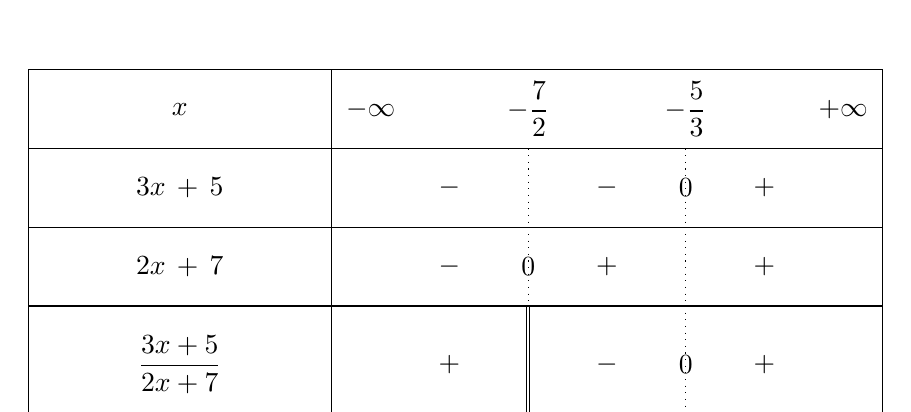
\begin{tikzpicture}
\tkzTabInit[lgt=3.85,espcl=2]{$x$ / 1, $3 x + 5$ / 1, $2 x + 7$ / 1, $\dfrac{3 x + 5}{2 x + 7}$ / 1.5}{$-\infty$, $- \dfrac{7}{2}$, $- \dfrac{5}{3}$, $+\infty$}
\tkzTabLine{, -, t, -, z, +}
\tkzTabLine{, -, z, +, t, +}
\tkzTabLine{, +, d, -, z, +}
\end{tikzpicture}
\end{center}
\par\smallskip
\begin{center}$S = \left] -\infty \,;\, - \dfrac{7}{2} \right[ \cup \left] - \dfrac{5}{3} \,;\, +\infty \right[$\end{center}\par\medskip
\noindent\textbf{2)}\par\smallskip
\begin{center}
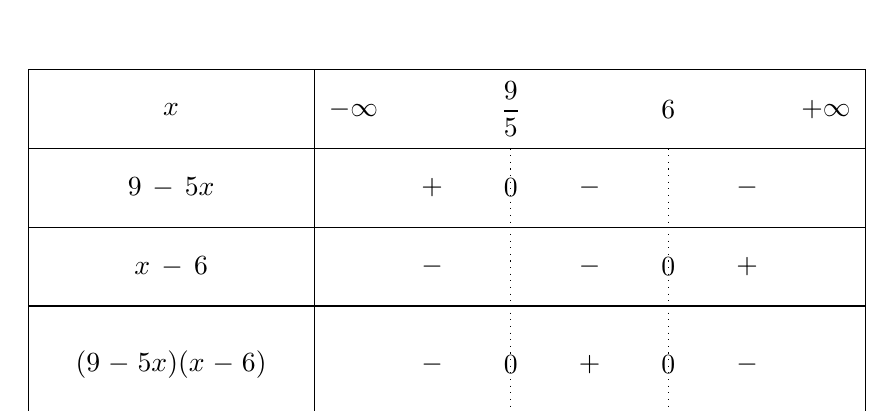
\begin{tikzpicture}
\tkzTabInit[lgt=3.63,espcl=2]{$x$ / 1, $9 - 5 x$ / 1, $x - 6$ / 1, $(9 - 5 x)(x - 6)$ / 1.5}{$-\infty$, $\dfrac{9}{5}$, $6$, $+\infty$}
\tkzTabLine{, +, z, -, t, -}
\tkzTabLine{, -, t, -, z, +}
\tkzTabLine{, -, z, +, z, -}
\end{tikzpicture}
\end{center}
\par\smallskip
\begin{center}$S = \left[ \dfrac{9}{5} \,;\, 6 \right]$\end{center}\par\medskip
\noindent\textbf{3)}\par\smallskip
\begin{center}
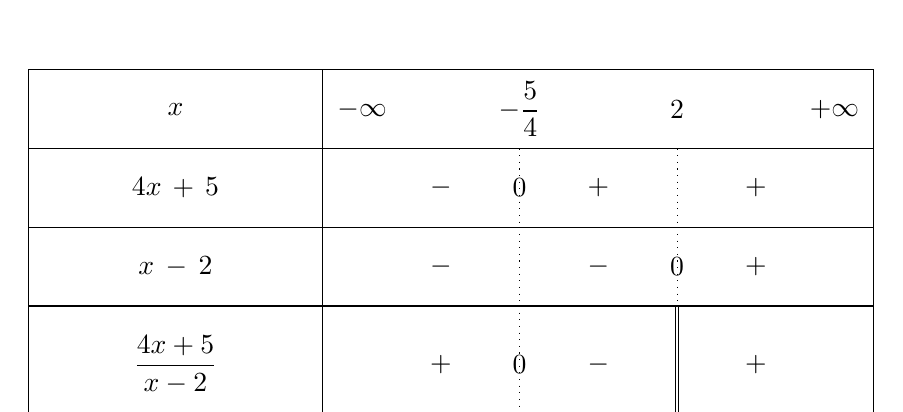
\begin{tikzpicture}
\tkzTabInit[lgt=3.74,espcl=2]{$x$ / 1, $4 x + 5$ / 1, $x - 2$ / 1, $\dfrac{4 x + 5}{x - 2}$ / 1.5}{$-\infty$, $- \dfrac{5}{4}$, $2$, $+\infty$}
\tkzTabLine{, -, z, +, t, +}
\tkzTabLine{, -, t, -, z, +}
\tkzTabLine{, +, z, -, d, +}
\end{tikzpicture}
\end{center}
\par\smallskip
\begin{center}$S = \left] - \dfrac{5}{4} \,;\, 2 \right[$\end{center}\par\medskip
\noindent\textbf{4)}\par\smallskip
\begin{center}
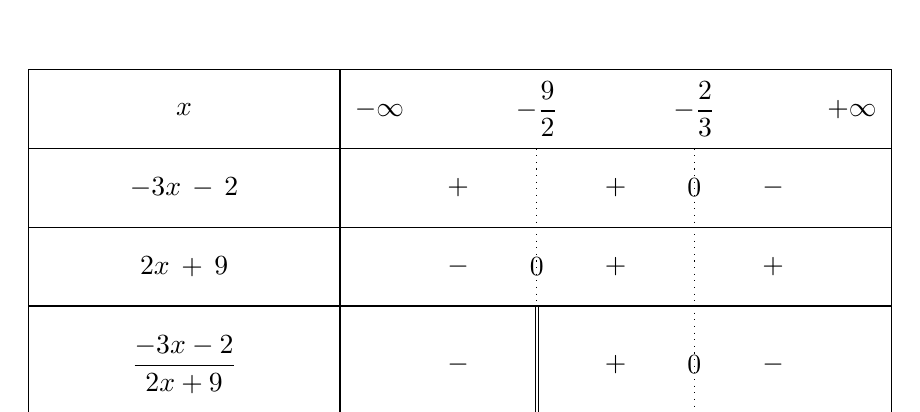
\begin{tikzpicture}
\tkzTabInit[lgt=3.96,espcl=2]{$x$ / 1, $- 3 x - 2$ / 1, $2 x + 9$ / 1, $\dfrac{- 3 x - 2}{2 x + 9}$ / 1.5}{$-\infty$, $- \dfrac{9}{2}$, $- \dfrac{2}{3}$, $+\infty$}
\tkzTabLine{, +, t, +, z, -}
\tkzTabLine{, -, z, +, t, +}
\tkzTabLine{, -, d, +, z, -}
\end{tikzpicture}
\end{center}
\par\smallskip
\begin{center}$S = \left] - \dfrac{9}{2} \,;\, - \dfrac{2}{3} \right[$\end{center}\par\medskip
\medskip

\noindent\textbf{Exercice 15}\par
\smallskip
\begin{enumerate}
\item $\dfrac{10^{-2} \times 10^{-1}}{10^{2}} = 10^{-5}$
\item $\dfrac{10^{-3} \times (10^{1})^{2}}{10^{1}} = 10^{-2}$
\item $\dfrac{10^{2} \times 10^{-1}}{10^{2}} = 10^{-1}$
\item $\dfrac{10^{3} \times (10^{3})^{3}}{10^{4}} = 10^{8}$
\end{enumerate}
\medskip

\noindent\textbf{Exercice 16}\par
\smallskip
\begin{enumerate}
\item $6 \sqrt{7}$
\item $10 \sqrt{5}$
\item $\sqrt{3} + 8 \sqrt{10}$
\item $0$
\item $3 \sqrt{2}$
\item $176 - 10 \sqrt{7}$
\end{enumerate}
\medskip

\noindent\textbf{Exercice 17}\par
\smallskip
\textbf{1)}
\begin{enumerate}
\item $\overrightarrow{\ensuremath{\mathrm{A}}\ensuremath{\mathrm{B}}}(1\,;\,3)$
\item $\overrightarrow{\ensuremath{\mathrm{A}}\ensuremath{\mathrm{B}}}(6\,;\,6)$
\item $\overrightarrow{\ensuremath{\mathrm{A}}\ensuremath{\mathrm{B}}}(-7\,;\,8)$
\end{enumerate}
\textbf{2)}
\begin{enumerate}
\item $\ensuremath{\mathrm{M}}\left(- \dfrac{5}{2}\,;\,0\right)$
\item $\ensuremath{\mathrm{M}}\left(1\,;\,-2\right)$
\end{enumerate}
\textbf{3)}
\begin{enumerate}
\item $\det(\vec{u},\vec{v}) = 2\times(1)-(-2)\times1 = 4$. Non.
\item $\det(\vec{u},\vec{v}) = -5\times(12)-(-4)\times15 = 0$. Oui.
\end{enumerate}
\medskip

\noindent\textbf{Exercice 18}\par
\smallskip
\textbf{1)}
\begin{enumerate}
\item $m = \dfrac{5-1}{-3-0} = - \dfrac{4}{3}$ donc $y = - \dfrac{4}{3}x + 1$
\item $m = \dfrac{-5-3}{1--4} = - \dfrac{8}{5}$ donc $y = - \dfrac{8}{5}x - \dfrac{17}{5}$
\item $m = \dfrac{-2-2}{-1--5} = -1$ donc $y = -1x - 3$
\end{enumerate}
\textbf{2)}
\begin{enumerate}
\item On cherche les couples $(x\,;\,y)$ vérifiant les deux équations :

$-x - 1 = -3x$

$\Leftrightarrow 2x = 1$

$\Leftrightarrow x = \dfrac{1}{2}$

puis $y = -(\dfrac{1}{2}) - 1 = - \dfrac{3}{2}$

Donc le point d'intersection est $\left(\dfrac{1}{2}\,;\,- \dfrac{3}{2}\right)$.
\item On cherche les couples $(x\,;\,y)$ vérifiant les deux équations :

$-4x - 2 = x - 4$

$\Leftrightarrow -5x = -2$

$\Leftrightarrow x = \dfrac{2}{5}$

puis $y = -4 \times (\dfrac{2}{5}) - 2 = - \dfrac{18}{5}$

Donc le point d'intersection est $\left(\dfrac{2}{5}\,;\,- \dfrac{18}{5}\right)$.
\end{enumerate}
\medskip

\newpage
\begin{center}
\textbf{Sujet numéro 5}
\\(à rendre avec la copie)
\end{center}


\noindent\textbf{Exercice 1} -- Développer les expressions suivantes.
\begin{enumerate}
\item $2(6x + 1)$
\item $4(6x + 8)$
\item $-9(-6x - 9)$
\item $2(3x - 7)$
\end{enumerate}
\noindent\textbf{Exercice} -- Factoriser les expressions suivantes.
\begin{enumerate}
\item $-36x - 42$
\item $16x - 14$
\item $-32x + 32$
\item $-24x - 36$
\end{enumerate}
\bigskip

\noindent\textbf{Exercice 2} -- Calculer en respectant les priorités opératoires.
\begin{enumerate}
\item $(13 + 9) \times 7$
\item $(2 + 7) \times 2$
\item $2 \times (9 + 10) - 9$
\item $6 \times (9 + 10) - 2$
\item $(2 + 10) \times 9$
\item $3 \times (9 - 6) - 2$
\end{enumerate}
\bigskip

\noindent\textbf{Exercice 3} -- Calculer les expressions suivantes.
\begin{enumerate}
\item $(-1) + (+5) + (-17)$
\item $(-5) + (-11) + (+4)$
\item $(-14) + (-6) + (-14)$
\item $(+10) + (+5) + (-9)$
\item $(-10) - (+3) - (+10)$
\item $(-17) - (+1) + (-16)$
\item $(-11) + (-9) - (-2)$
\item $(-19) + (-19) + (+8)$
\end{enumerate}
\bigskip

\noindent\textbf{Exercice 4} -- Développer et réduire.
\begin{enumerate}
\item $-6x(4 - 5x)$
\item $-5x(7x - 5)$
\item $(4x - 4)(8x - 2)$
\item $(-8x - 8)(-7x - 6)$
\item $(7 - 8x)(9 - 7x)$
\item $(5x + 3)(9x - 2)$
\end{enumerate}
\bigskip

\noindent\textbf{Exercice 5} -- Réduire les expressions suivantes.
\begin{enumerate}
\item $(4x - 3)-(5 - 3x)$
\item $-(-6x - 7)-(4 - 4x)$
\item $-(7x + 5)-(-6x - 2)$
\item $(2x - 3)+(-7x - 4)$
\item $-(7 - 9x)+(-6x - 6)$
\end{enumerate}
\bigskip

\noindent\textbf{Exercice 6} -- Théorème de Pythagore.
\medskip

\noindent\textbf{1.} Le triangle \ensuremath{\mathrm{A}}\ensuremath{\mathrm{B}}\ensuremath{\mathrm{C}} est rectangle en \ensuremath{\mathrm{B}}. On donne $\ensuremath{\mathrm{A}}\ensuremath{\mathrm{B}} = 6~\text{cm}$ et $\ensuremath{\mathrm{B}}\ensuremath{\mathrm{C}} = 8~\text{cm}$.

\begin{center}
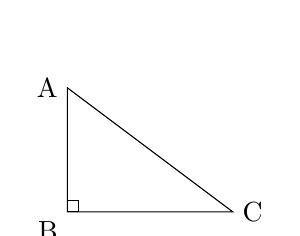
\begin{tikzpicture}[scale=0.35]
\draw (0,4.50) node[left]{A} -- (0,0) node[below left]{B} -- (6.00,0) node[right]{C} -- cycle;
\draw (0,0) rectangle (0.4,0.4);
\end{tikzpicture}
\end{center}

Calculer la valeur exacte de $\ensuremath{\mathrm{A}}\ensuremath{\mathrm{C}}$.

\medskip

\noindent\textbf{2.} Le triangle \ensuremath{\mathrm{D}}\ensuremath{\mathrm{E}}\ensuremath{\mathrm{F}} est rectangle en \ensuremath{\mathrm{E}}. On donne $\ensuremath{\mathrm{D}}\ensuremath{\mathrm{F}} = 15~\text{cm}$ et $\ensuremath{\mathrm{D}}\ensuremath{\mathrm{E}} = 9~\text{cm}$.

\begin{center}
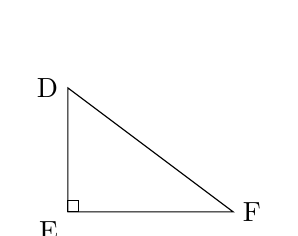
\begin{tikzpicture}[scale=0.35]
\draw (0,4.50) node[left]{D} -- (0,0) node[below left]{E} -- (6.00,0) node[right]{F} -- cycle;
\draw (0,0) rectangle (0.4,0.4);
\end{tikzpicture}
\end{center}

Calculer la valeur exacte de $\ensuremath{\mathrm{E}}\ensuremath{\mathrm{F}}$.

\medskip

\noindent\textbf{3.} Le triangle \ensuremath{\mathrm{M}}\ensuremath{\mathrm{N}}\ensuremath{\mathrm{P}} est rectangle en \ensuremath{\mathrm{N}}. On donne $\ensuremath{\mathrm{M}}\ensuremath{\mathrm{N}} = 6~\text{cm}$ et $\ensuremath{\mathrm{N}}\ensuremath{\mathrm{P}} = 11~\text{cm}$.

\begin{center}
\begin{tikzpicture}[scale=0.35]
\draw (0,3.27) node[left]{M} -- (0,0) node[below left]{N} -- (6.00,0) node[right]{P} -- cycle;
\draw (0,0) rectangle (0.4,0.4);
\end{tikzpicture}
\end{center}

Calculer la valeur exacte de $\ensuremath{\mathrm{M}}\ensuremath{\mathrm{P}}$.

\medskip

\noindent\textbf{4.} Le triangle \ensuremath{\mathrm{R}}\ensuremath{\mathrm{S}}\ensuremath{\mathrm{T}} est rectangle en \ensuremath{\mathrm{S}}. On donne $\ensuremath{\mathrm{R}}\ensuremath{\mathrm{T}} = 12~\text{cm}$ et $\ensuremath{\mathrm{R}}\ensuremath{\mathrm{S}} = 6~\text{cm}$.

\begin{center}
\begin{tikzpicture}[scale=0.35]
\draw (0,3.00) node[left]{R} -- (0,0) node[below left]{S} -- (6.00,0) node[right]{T} -- cycle;
\draw (0,0) rectangle (0.4,0.4);
\end{tikzpicture}
\end{center}

Calculer la valeur exacte de $\ensuremath{\mathrm{S}}\ensuremath{\mathrm{T}}$.

\medskip
\bigskip

\noindent\textbf{Exercice 7} -- Théorème de Thalès

\medskip
\noindent\textbf{1.} Les droites (\ensuremath{\mathrm{B}}\ensuremath{\mathrm{B}^\prime}) et (\ensuremath{\mathrm{C}}\ensuremath{\mathrm{C}^\prime}) sont parallèles. \ensuremath{\mathrm{A}}\ensuremath{\mathrm{B}} = 2, \ensuremath{\mathrm{A}}\ensuremath{\mathrm{B}^\prime} = 5, \ensuremath{\mathrm{A}}\ensuremath{\mathrm{C}} = 4.

\begin{center}
\begin{tikzpicture}[scale=0.8]
\draw [thick] (0.000,0.000)--(2.000,0.000);
\draw [thick] (2.000,0.000)--(4.000,0.000);
\draw [thick] (0.000,0.000)--(4.045,2.939);
\draw [thick] (4.045,2.939)--(8.090,5.878);
\draw [thick] (2.000,0.000)--(4.045,2.939);
\draw [thick] (4.000,0.000)--(8.090,5.878);
\draw (-0.400,-0.300) node {A};
\draw (2.000,-0.500) node {B};
\draw (4.000,-0.500) node {C};
\draw (3.645,3.239) node {B'};
\draw (8.390,6.178) node {C'};
\end{tikzpicture}
\end{center}
Déterminer en justifiant la valeur exacte de \ensuremath{\mathrm{A}}\ensuremath{\mathrm{C}^\prime}.

\bigskip
\noindent\textbf{2.} Les droites (\ensuremath{\mathrm{B}}\ensuremath{\mathrm{B}^\prime}) et (\ensuremath{\mathrm{C}}\ensuremath{\mathrm{C}^\prime}) sont parallèles. \ensuremath{\mathrm{A}}\ensuremath{\mathrm{B}} = 2, \ensuremath{\mathrm{A}}\ensuremath{\mathrm{B}^\prime} = 4, \ensuremath{\mathrm{A}}\ensuremath{\mathrm{C}} = 6.

\begin{center}
\begin{tikzpicture}[scale=0.8]
\draw [thick] (0.000,0.000)--(2.000,0.000);
\draw [thick] (2.000,0.000)--(6.000,0.000);
\draw [thick] (0.000,0.000)--(2.828,2.828);
\draw [thick] (2.828,2.828)--(8.485,8.485);
\draw [thick] (2.000,0.000)--(2.828,2.828);
\draw [thick] (6.000,0.000)--(8.485,8.485);
\draw (-0.400,-0.300) node {A};
\draw (2.000,-0.500) node {B};
\draw (6.000,-0.500) node {C};
\draw (2.428,3.128) node {B'};
\draw (8.785,8.785) node {C'};
\end{tikzpicture}
\end{center}
Déterminer en justifiant la valeur exacte de \ensuremath{\mathrm{A}}\ensuremath{\mathrm{C}^\prime}.

\bigskip
\noindent\textbf{3.} Les droites (\ensuremath{\mathrm{B}}\ensuremath{\mathrm{B}^\prime}) et (\ensuremath{\mathrm{C}}\ensuremath{\mathrm{C}^\prime}) sont parallèles. \ensuremath{\mathrm{A}}\ensuremath{\mathrm{C}} = 6, \ensuremath{\mathrm{A}}\ensuremath{\mathrm{B}^\prime} = 4, \ensuremath{\mathrm{A}}\ensuremath{\mathrm{B}} = 2.

\begin{center}
\begin{tikzpicture}[scale=0.8]
\draw [thick] (0.000,0.000)--(2.000,0.000);
\draw [thick] (2.000,0.000)--(-6.000,0.000);
\draw [thick] (0.000,0.000)--(3.464,2.000);
\draw [thick] (3.464,2.000)--(-10.392,-6.000);
\draw [thick] (2.000,0.000)--(3.464,2.000);
\draw [thick] (-6.000,0.000)--(-10.392,-6.000);
\draw (0.100,-0.500) node {A};
\draw (2.300,0.000) node {B};
\draw (-6.500,0.000) node {C};
\draw (3.764,2.200) node {B'};
\draw (-10.892,-6.200) node {C'};
\end{tikzpicture}
\end{center}
Déterminer en justifiant la valeur exacte de \ensuremath{\mathrm{A}}\ensuremath{\mathrm{C}^\prime}.

\bigskip
\noindent\textbf{4.} Les droites (\ensuremath{\mathrm{B}}\ensuremath{\mathrm{B}^\prime}) et (\ensuremath{\mathrm{C}}\ensuremath{\mathrm{C}^\prime}) sont parallèles. \ensuremath{\mathrm{A}}\ensuremath{\mathrm{B}} = 5, \ensuremath{\mathrm{A}}\ensuremath{\mathrm{C}} = 9, \ensuremath{\mathrm{A}}\ensuremath{\mathrm{B}^\prime} = 4.

\begin{center}
\begin{tikzpicture}[scale=0.8]
\draw [thick] (0.000,0.000)--(5.000,0.000);
\draw [thick] (5.000,0.000)--(-9.000,0.000);
\draw [thick] (0.000,0.000)--(3.464,2.000);
\draw [thick] (3.464,2.000)--(-6.235,-3.600);
\draw [thick] (5.000,0.000)--(3.464,2.000);
\draw [thick] (-9.000,0.000)--(-6.235,-3.600);
\draw (0.100,-0.500) node {A};
\draw (5.300,0.000) node {B};
\draw (-9.500,0.000) node {C};
\draw (3.764,2.200) node {B'};
\draw (-6.735,-3.800) node {C'};
\end{tikzpicture}
\end{center}
Déterminer en justifiant la valeur exacte de \ensuremath{\mathrm{A}}\ensuremath{\mathrm{C}^\prime}.
\bigskip

\noindent\textbf{Exercice 8} -- Résoudre les équations suivantes.
\begin{enumerate}
\item $9x = 3$
\item $10 - 3x = -6$
\item $-8x - 6 = 11$
\item $-4x - 9 = -3x - 4$
\item $-7x - 9 = 7 - 8x$
\end{enumerate}
\bigskip

\noindent\textbf{Exercice 9} -- Résoudre les équations suivantes.
\begin{enumerate}
\item $(2 - 7x)(5 - 3x) = 0$
\item $(-5x - 6)(2x - 6) = 0$
\item $(-3x - 7)(6x + 4) = 0$
\item $(-6x - 7)(5x - 6) = 0$
\end{enumerate}
\bigskip

\noindent\textbf{Exercice 10} -- Calculer et simplifier.
\begin{enumerate}
\item $\dfrac{8}{7} - \dfrac{8}{2}$
\item $\dfrac{1}{7} + \dfrac{9}{8}$
\item $\dfrac{2}{5} - \dfrac{2}{2} \times \dfrac{3}{3}$
\item $\dfrac{4}{6} - \dfrac{1}{2} \times \dfrac{5}{5}$
\item $\dfrac{2 + \dfrac{2}{5}}{\dfrac{4}{2} - \dfrac{2}{3}}$
\end{enumerate}
\bigskip

\noindent\textbf{Exercice 11} -- Factoriser les expressions suivantes.
\begin{enumerate}
\item $(-6x - 5)(-3x - 6) - (-6x - 5)(-4x - 5)$
\item $(2x + 7)(2 - 2x) - (2x + 7)(-6x - 1)$
\item $(5x + 5)(3 - 7x) - (5x + 5)(2x + 6)$
\end{enumerate}
\bigskip

\noindent\textbf{Exercice 12} -- Factoriser en utilisant une identité remarquable.
\begin{enumerate}
\item $9x^2 - 18x + 9$
\item $(x + 7)^2 - (2x + 2)^2$
\item $(x + 2)^2 - (5x + 1)^2$
\end{enumerate}
\bigskip

\noindent\textbf{Exercice 13} -- Résoudre les inéquations suivantes.
\begin{enumerate}
\item $7 x > 4$
\item $- 6 x > 7$
\item $- 3 x - 2 \leq -2$
\item $9 x - 4 < 9$
\item $- 7 x - 5 > 4 x - 9$
\item $- 6 x - 8 \geq - 2 x - 6$
\end{enumerate}
\bigskip

\noindent\textbf{Exercice 14} -- Résoudre à l'aide d'un tableau de signes.
\begin{enumerate}
\item $\left(3 x - 9\right) \left(5 x + 4\right) \geq 0$
\item $\dfrac{5 - 3 x}{2 - 4 x} \geq 0$
\item $\dfrac{3 x - 1}{- x - 2} < 0$
\item $\dfrac{3 x - 8}{- 2 x - 6} \leq 0$
\end{enumerate}
\bigskip

\noindent\textbf{Exercice 15} -- Écrire sous la forme d'une unique puissance de 10.
\begin{enumerate}
\item $\dfrac{10^{2} \times 10^{1}}{10^{2}}$
\item $\dfrac{10^{-3} \times (10^{3})^{3}}{10^{1}}$
\item $\dfrac{10^{1} \times 10^{-2}}{10^{3}}$
\item $\dfrac{10^{-2} \times (10^{3})^{3}}{10^{4}}$
\end{enumerate}
\bigskip

\noindent\textbf{Exercice 16} -- Calculer et simplifier.
\begin{enumerate}
\item $\sqrt{72}$
\item $\sqrt{700}$
\item $4\sqrt{7} + 3\sqrt{11} + \sqrt{7} - 2\sqrt{11}$
\item $2\sqrt{11} - 4\sqrt{10} - 5\sqrt{11} + \sqrt{10}$
\item $-3\sqrt{252} + 4\sqrt{7} - \sqrt{28} - \sqrt{63}$
\item $(3 - 5\sqrt{3})^2$
\end{enumerate}
\bigskip

\noindent\textbf{Exercice 17} -- Vecteurs et coordonnées.\\
\medskip
\noindent\textbf{1)} Calculer les coordonnées de $\overrightarrow{\ensuremath{\mathrm{A}}\ensuremath{\mathrm{B}}}$.
\begin{enumerate}
\item $\ensuremath{\mathrm{A}}(2\,;\,-2)$ et $\ensuremath{\mathrm{B}}(-4\,;\,-4)$
\item $\ensuremath{\mathrm{A}}(2\,;\,4)$ et $\ensuremath{\mathrm{B}}(-2\,;\,4)$
\item $\ensuremath{\mathrm{A}}(5\,;\,2)$ et $\ensuremath{\mathrm{B}}(-1\,;\,-4)$
\end{enumerate}
\medskip
\noindent\textbf{2)} Calculer les coordonnées du milieu de $[\ensuremath{\mathrm{A}}\ensuremath{\mathrm{B}}]$.
\begin{enumerate}
\item $\ensuremath{\mathrm{A}}(7\,;\,-6)$ et $\ensuremath{\mathrm{B}}(6\,;\,-7)$
\item $\ensuremath{\mathrm{A}}(8\,;\,8)$ et $\ensuremath{\mathrm{B}}(-5\,;\,3)$
\end{enumerate}
\medskip
\noindent\textbf{3)} Les vecteurs $\vec{u}$ et $\vec{v}$ sont-ils colinéaires ?
\begin{enumerate}
\item $\vec{u}(-3\,;\,5)$ et $\vec{v}(-3\,;\,5)$
\item $\vec{u}(-5\,;\,-5)$ et $\vec{v}(15\,;\,15)$
\end{enumerate}
\bigskip

\noindent\textbf{Exercice 18} -- Équations de droites.
\medskip
\noindent\textbf{1)} Déterminer l'équation réduite de la droite $(\ensuremath{\mathrm{A}}\ensuremath{\mathrm{B}})$.
\begin{enumerate}
\item $\ensuremath{\mathrm{A}}(-5\,;\,-4)$ et $\ensuremath{\mathrm{B}}(-2\,;\,4)$
\item $\ensuremath{\mathrm{A}}(-1\,;\,-3)$ et $\ensuremath{\mathrm{B}}(-4\,;\,-3)$
\item $\ensuremath{\mathrm{A}}(3\,;\,0)$ et $\ensuremath{\mathrm{B}}(-1\,;\,-3)$
\end{enumerate}
\noindent\textbf{2)} Déterminer le point d'intersection.
\begin{enumerate}
\item $(d_1): y = x + 2$ et $(d_2): y = 5x - 3$
\item $(d_1): y = 4x + 2$ et $(d_2): y = -2x + 3$
\end{enumerate}
\bigskip

\vfill
\begin{flushright}
\qrset{height=1.5cm}
\qrset{level=M}
\qrcode{Ex1: 12x + 2 | 24x + 32 | 54x + 81 | 6x - 14 | 6(-6x - 7) | 2(8x - 7) | 4(-8x + 8) | 4(-6x - 9)  //  Ex2: 154 | 18 | 29 | 112 | 108 | 7  //  Ex3: -13 | -12 | -34 | 6 | -23 | -34 | -18 | -30  //  Ex4: 30x^2 - 24x | -35x^2 + 25x | 32x^2 - 40x + 8 | 56x^2 + 104x + 48 | 56x^2 - 121x + 63 | 45x^2 + 17x - 6  //  Ex5: 7x - 8 | 10x + 3 | -x - 3 | -5x - 7 | 3x - 13  //  Ex6: sqrt(100)~ cm | sqrt(144)~ cm | sqrt(157)$ cm | sqrt(108)$ cm  //  Ex7: 10 | 12 | 12 | 36/5  //  Ex8: S = (1)/(3) | S = (16)/(3) | S = - (17)/(8) | S = -5 | S = 16  //  Ex9: S = (2)/(7) ; (5)/(3) | S = - (6)/(5) ; 3 | S = - (7)/(3) ; - (2)/(3) | S = - (7)/(6) ; (6)/(5)  //  Ex10: - (20)/(7) | (71)/(56) | - (3)/(5) | (1)/(6) | (9)/(5)  //  Ex11: (-6x - 5)(x - 1) | (2x + 7)(4x + 3) | (5x + 5)(-9x - 3)  //  Ex12: (3x - 3)^2 | -3(x - 5)(x + 3) | -3(2x + 1)(4x - 1)  //  Ex13: ] (4)/(7) ; +inf [ | ] -inf ; - (7)/(6) [ | [ 0 ; +inf [ | ] -inf ; (13)/(9) [ | ] -inf ; (4)/(11) [ | ] -inf ; - (1)/(2) ]  //  Ex14: ] -inf ; - (4)/(5) ] U [ 3 ; +inf [ | ] -inf ; (1)/(2) [ U [ (5)/(3) ; +inf [ | ] -inf ; -2 [ U ] (1)/(3) ; +inf [ | ] -inf ; -3 [ U [ (8)/(3) ; +inf [  //  Ex15: 10^1 | 10^5 | 10^-4 | 10^3  //  Ex16: 6 sqrt(2) | 10 sqrt(7) | sqrt(11) + 5 sqrt(7) | - 3 sqrt(11) - 3 sqrt(10) | - 19 sqrt(7) | 84 - 30 sqrt(3)  //  Ex17: AB(-6;-2) | AB(-4;0) | AB(-6;-6)  //  Ex18: y = (8)/(3)x + (28)/(3) | y = 0x - 3 | y = (3)/(4)x - (9)/(4)}
\end{flushright}
\newpage
\begin{center}
\textbf{Corrigé numéro 5}\\
\end{center}

\noindent\textbf{Exercice 1}\par
\smallskip
\begin{enumerate}
\item $2(6x + 1) = 12x + 2$
\item $4(6x + 8) = 24x + 32$
\item $-9(-6x - 9) = 54x + 81$
\item $2(3x - 7) = 6x - 14$
\end{enumerate}
\begin{enumerate}
\item $-36x - 42 = 6(-6x - 7)$
\item $16x - 14 = 2(8x - 7)$
\item $-32x + 32 = 4(-8x + 8)$
\item $-24x - 36 = 4(-6x - 9)$
\end{enumerate}
\medskip

\noindent\textbf{Exercice 2}\par
\smallskip
\begin{enumerate}
\item $(13 + 9) \times 7$

$= 22 \times 7$

$= 154$
\item $(2 + 7) \times 2$

$= 9 \times 2$

$= 18$
\item $2 \times (9 + 10) - 9$

$= 2 \times 19 - 9$

$= 38 - 9$

$= 29$
\item $6 \times (9 + 10) - 2$

$= 6 \times 19 - 2$

$= 114 - 2$

$= 112$
\item $(2 + 10) \times 9$

$= 12 \times 9$

$= 108$
\item $3 \times (9 - 6) - 2$

$= 3 \times 3 - 2$

$= 9 - 2$

$= 7$
\end{enumerate}
\medskip

\noindent\textbf{Exercice 3}\par
\smallskip
\begin{enumerate}
\item $(-1) + (+5) + (-17) = -13$
\item $(-5) + (-11) + (+4) = -12$
\item $(-14) + (-6) + (-14) = -34$
\item $(+10) + (+5) + (-9) = 6$
\item $(-10) - (+3) - (+10) = -23$
\item $(-17) - (+1) + (-16) = -34$
\item $(-11) + (-9) - (-2) = -18$
\item $(-19) + (-19) + (+8) = -30$
\end{enumerate}
\medskip

\noindent\textbf{Exercice 4}\par
\smallskip
\begin{enumerate}
\item $-6x(4 - 5x) = 30x^2 - 24x$
\item $-5x(7x - 5) = -35x^2 + 25x$
\item $(4x - 4)(8x - 2) = 32x^2 - 40x + 8$
\item $(-8x - 8)(-7x - 6) = 56x^2 + 104x + 48$
\item $(7 - 8x)(9 - 7x) = 56x^2 - 121x + 63$
\item $(5x + 3)(9x - 2) = 45x^2 + 17x - 6$
\end{enumerate}
\medskip

\noindent\textbf{Exercice 5}\par
\smallskip
\begin{enumerate}
\item $(4x - 3)-(5 - 3x) = 7x - 8$
\item $-(-6x - 7)-(4 - 4x) = 10x + 3$
\item $-(7x + 5)-(-6x - 2) = -x - 3$
\item $(2x - 3)+(-7x - 4) = -5x - 7$
\item $-(7 - 9x)+(-6x - 6) = 3x - 13$
\end{enumerate}
\medskip

\noindent\textbf{Exercice 6}\par
\smallskip
\textbf{1.} D'après le théorème de Pythagore dans le triangle \ensuremath{\mathrm{A}}\ensuremath{\mathrm{B}}\ensuremath{\mathrm{C}} rectangle en \ensuremath{\mathrm{B}} :

$\ensuremath{\mathrm{A}}\ensuremath{\mathrm{C}}^2 = \ensuremath{\mathrm{A}}\ensuremath{\mathrm{B}}^2 + \ensuremath{\mathrm{B}}\ensuremath{\mathrm{C}}^2$

$\ensuremath{\mathrm{A}}\ensuremath{\mathrm{C}}^2 = (6~\text{cm})^2 + (8~\text{cm})^2 = 36~\text{cm}^2 + 64~\text{cm}^2 = 100~\text{cm}^2$

Donc $\ensuremath{\mathrm{A}}\ensuremath{\mathrm{C}} = \sqrt{100}~\text{cm} = 10~\text{cm}$

\medskip
\textbf{2.} D'après le théorème de Pythagore dans le triangle \ensuremath{\mathrm{D}}\ensuremath{\mathrm{E}}\ensuremath{\mathrm{F}} rectangle en \ensuremath{\mathrm{E}} :

$\ensuremath{\mathrm{D}}\ensuremath{\mathrm{F}}^2 = \ensuremath{\mathrm{D}}\ensuremath{\mathrm{E}}^2 + \ensuremath{\mathrm{E}}\ensuremath{\mathrm{F}}^2$

Donc $\ensuremath{\mathrm{E}}\ensuremath{\mathrm{F}}^2 = \ensuremath{\mathrm{D}}\ensuremath{\mathrm{F}}^2 - \ensuremath{\mathrm{D}}\ensuremath{\mathrm{E}}^2 = (15~\text{cm})^2 - (9~\text{cm})^2 = 225~\text{cm}^2 - 81~\text{cm}^2 = 144~\text{cm}^2$

Donc $\ensuremath{\mathrm{E}}\ensuremath{\mathrm{F}} = \sqrt{144}~\text{cm} = 12~\text{cm}$

\medskip
\textbf{3.} D'après le théorème de Pythagore :

$\ensuremath{\mathrm{M}}\ensuremath{\mathrm{P}}^2 = (6~\text{cm})^2 + (11~\text{cm})^2 = 36~\text{cm}^2 + 121~\text{cm}^2 = 157~\text{cm}^2$

Donc $\ensuremath{\mathrm{M}}\ensuremath{\mathrm{P}} = \sqrt{157}$ cm

\medskip
\textbf{4.} D'après le théorème de Pythagore :

$\ensuremath{\mathrm{R}}\ensuremath{\mathrm{T}}^2 = \ensuremath{\mathrm{R}}\ensuremath{\mathrm{S}}^2 + \ensuremath{\mathrm{S}}\ensuremath{\mathrm{T}}^2$

Donc $\ensuremath{\mathrm{S}}\ensuremath{\mathrm{T}}^2 = (12~\text{cm})^2 - (6~\text{cm})^2 = 144~\text{cm}^2 - 36~\text{cm}^2 = 108~\text{cm}^2$

Donc $\ensuremath{\mathrm{S}}\ensuremath{\mathrm{T}} = \sqrt{108}$ cm

\medskip
\medskip

\noindent\textbf{Exercice 7}\par
\smallskip
\textbf{1.} Comme (\ensuremath{\mathrm{B}}\ensuremath{\mathrm{B}^\prime}) et (\ensuremath{\mathrm{C}}\ensuremath{\mathrm{C}^\prime}) sont parallèles, d'après le théorème de Thalès : \[\dfrac{\ensuremath{\mathrm{A}}\ensuremath{\mathrm{C}^\prime}}{\ensuremath{\mathrm{A}}\ensuremath{\mathrm{C}}}=\dfrac{\ensuremath{\mathrm{A}}\ensuremath{\mathrm{B}^\prime}}{\ensuremath{\mathrm{A}}\ensuremath{\mathrm{B}}}=\dfrac{5}{2}.\]Donc \[\ensuremath{\mathrm{A}}\ensuremath{\mathrm{C}^\prime}=4\times\dfrac{5}{2}=10.\]\medskip
\textbf{2.} Comme (\ensuremath{\mathrm{B}}\ensuremath{\mathrm{B}^\prime}) et (\ensuremath{\mathrm{C}}\ensuremath{\mathrm{C}^\prime}) sont parallèles, d'après le théorème de Thalès : \[\dfrac{\ensuremath{\mathrm{A}}\ensuremath{\mathrm{C}^\prime}}{\ensuremath{\mathrm{A}}\ensuremath{\mathrm{C}}}=\dfrac{\ensuremath{\mathrm{A}}\ensuremath{\mathrm{B}^\prime}}{\ensuremath{\mathrm{A}}\ensuremath{\mathrm{B}}}=\dfrac{4}{2}.\]Donc \[\ensuremath{\mathrm{A}}\ensuremath{\mathrm{C}^\prime}=6\times\dfrac{4}{2}=12.\]\medskip
\textbf{3.} Comme (\ensuremath{\mathrm{B}}\ensuremath{\mathrm{B}^\prime}) et (\ensuremath{\mathrm{C}}\ensuremath{\mathrm{C}^\prime}) sont parallèles, d'après le théorème de Thalès : \[\dfrac{\ensuremath{\mathrm{A}}\ensuremath{\mathrm{C}^\prime}}{\ensuremath{\mathrm{A}}\ensuremath{\mathrm{C}}}=\dfrac{\ensuremath{\mathrm{A}}\ensuremath{\mathrm{B}^\prime}}{\ensuremath{\mathrm{A}}\ensuremath{\mathrm{B}}}=\dfrac{4}{2}.\]Donc \[\ensuremath{\mathrm{A}}\ensuremath{\mathrm{C}^\prime}=6\times\dfrac{4}{2}=12.\]\medskip
\textbf{4.} Comme (\ensuremath{\mathrm{B}}\ensuremath{\mathrm{B}^\prime}) et (\ensuremath{\mathrm{C}}\ensuremath{\mathrm{C}^\prime}) sont parallèles, d'après le théorème de Thalès : \[\dfrac{\ensuremath{\mathrm{A}}\ensuremath{\mathrm{C}^\prime}}{\ensuremath{\mathrm{A}}\ensuremath{\mathrm{C}}}=\dfrac{\ensuremath{\mathrm{A}}\ensuremath{\mathrm{B}^\prime}}{\ensuremath{\mathrm{A}}\ensuremath{\mathrm{B}}}=\dfrac{4}{5}.\]Donc \[\ensuremath{\mathrm{A}}\ensuremath{\mathrm{C}^\prime}=9\times\dfrac{4}{5}=\dfrac{36}{5}.\]\medskip
\medskip

\noindent\textbf{Exercice 8}\par
\smallskip
\begin{enumerate}
\item $9x = 3$

$\Leftrightarrow x = \dfrac{3}{9} = \dfrac{1}{3}$

L'ensemble des solutions est $S = \left\{\dfrac{1}{3}\right\}$.

\item $10 - 3x = -6$

$\Leftrightarrow -3x = -6 - (10) = -16$

$\Leftrightarrow x = \dfrac{-16}{-3} = \dfrac{16}{3}$

L'ensemble des solutions est $S = \left\{\dfrac{16}{3}\right\}$.

\item $-8x - 6 = 11$

$\Leftrightarrow -8x = 11 - (-6) = 17$

$\Leftrightarrow x = \dfrac{17}{-8} = - \dfrac{17}{8}$

L'ensemble des solutions est $S = \left\{- \dfrac{17}{8}\right\}$.

\item $-4x - 9 = -3x - 4$

$\Leftrightarrow -1x = 5$

$\Leftrightarrow x = \dfrac{5}{-1} = -5$

L'ensemble des solutions est $S = \left\{-5\right\}$.

\item $-7x - 9 = 7 - 8x$

$\Leftrightarrow 1x = 16$

$\Leftrightarrow x = \dfrac{16}{1} = 16$

L'ensemble des solutions est $S = \left\{16\right\}$.

\end{enumerate}
\medskip

\noindent\textbf{Exercice 9}\par
\smallskip
\begin{enumerate}
\item Un produit est nul si et seulement si l'un des facteurs est nul.

$\bullet\ 5 - 3x = 0 \Leftrightarrow x = \dfrac{5}{3}$

$\bullet\ 2 - 7x = 0 \Leftrightarrow x = \dfrac{2}{7}$

Donc $S = \left\{\dfrac{2}{7} \; ; \; \dfrac{5}{3}\right\}$

\item Un produit est nul si et seulement si l'un des facteurs est nul.

$\bullet\ 2x - 6 = 0 \Leftrightarrow x = 3$

$\bullet\ -5x - 6 = 0 \Leftrightarrow x = - \dfrac{6}{5}$

Donc $S = \left\{- \dfrac{6}{5} \; ; \; 3\right\}$

\item Un produit est nul si et seulement si l'un des facteurs est nul.

$\bullet\ -3x - 7 = 0 \Leftrightarrow x = - \dfrac{7}{3}$

$\bullet\ 6x + 4 = 0 \Leftrightarrow x = - \dfrac{2}{3}$

Donc $S = \left\{- \dfrac{7}{3} \; ; \; - \dfrac{2}{3}\right\}$

\item Un produit est nul si et seulement si l'un des facteurs est nul.

$\bullet\ 5x - 6 = 0 \Leftrightarrow x = \dfrac{6}{5}$

$\bullet\ -6x - 7 = 0 \Leftrightarrow x = - \dfrac{7}{6}$

Donc $S = \left\{- \dfrac{7}{6} \; ; \; \dfrac{6}{5}\right\}$

\end{enumerate}
\medskip

\noindent\textbf{Exercice 10}\par
\smallskip
\begin{enumerate}
\item $\dfrac{8 \times 2}{7 \times 2} - \dfrac{8 \times 7}{2 \times 7} = \dfrac{-40}{14} = - \dfrac{20}{7}$
\item $\dfrac{1 \times 8}{7 \times 8} + \dfrac{9 \times 7}{8 \times 7} = \dfrac{71}{56}$
\item $= \dfrac{2}{5} - 1$ (priorité $\times$)

$= \dfrac{2}{5} - \dfrac{5}{5} = \dfrac{-3}{5}$
\item $= \dfrac{4}{6} - \dfrac{1}{2}$ (priorité $\times$)

$= \dfrac{4}{6} - \dfrac{3}{6} = \dfrac{1}{6}$
\item Numérateur : $2 + \dfrac{2}{5} = \dfrac{2 \times 5 + 2}{5} = \dfrac{12}{5}$

Dénominateur : $\dfrac{4}{2} - \dfrac{2}{3} = \dfrac{4 \times 3 - 2 \times 2}{2 \times 3} = \dfrac{4}{3}$

$= \dfrac{12}{5} \div \dfrac{4}{3} = \dfrac{12}{5} \times \dfrac{3}{4} = \dfrac{9}{5}$
\end{enumerate}
\medskip

\noindent\textbf{Exercice 11}\par
\smallskip
\begin{enumerate}
\item $(-6x - 5)(x - 1)$
\item $(2x + 7)(4x + 3)$
\item $(5x + 5)(-9x - 3)$
\end{enumerate}
\medskip

\noindent\textbf{Exercice 12}\par
\smallskip
\begin{enumerate}
\item $(3x - 3)^2$
\item $-3(x - 5)(x + 3)$
\item $-3(2x + 1)(4x - 1)$
\end{enumerate}
\medskip

\noindent\textbf{Exercice 13}\par
\smallskip
\begin{enumerate}
\item $7x > 4$

$\Leftrightarrow x > \dfrac{4}{7}$

$S = \left] \dfrac{4}{7} \,;\, +\infty \right[$
\item $-6x > 7$

$\Leftrightarrow x < - \dfrac{7}{6}$

$S = \left] -\infty \,;\, - \dfrac{7}{6} \right[$
\item $- 3 x - 2 \leq -2$

$\Leftrightarrow -3x \leq -2 - (-2) = 0$

$\Leftrightarrow x \geq 0$

$S = \left[ 0 \,;\, +\infty \right[$
\item $9 x - 4 < 9$

$\Leftrightarrow 9x < 9 - (-4) = 13$

$\Leftrightarrow x < \dfrac{13}{9}$

$S = \left] -\infty \,;\, \dfrac{13}{9} \right[$
\item $- 7 x - 5 > 4 x - 9$

$\Leftrightarrow -11x > -4$

$\Leftrightarrow x < \dfrac{4}{11}$

$S = \left] -\infty \,;\, \dfrac{4}{11} \right[$
\item $- 6 x - 8 \geq - 2 x - 6$

$\Leftrightarrow -4x \geq 2$

$\Leftrightarrow x \leq - \dfrac{1}{2}$

$S = \left] -\infty \,;\, - \dfrac{1}{2} \right]$
\end{enumerate}
\medskip

\noindent\textbf{Exercice 14}\par
\smallskip
\noindent\textbf{1)}\par\smallskip
\begin{center}
\begin{tikzpicture}
\tkzTabInit[lgt=3.74,espcl=2]{$x$ / 1, $5 x + 4$ / 1, $3 x - 9$ / 1, $(5 x + 4)(3 x - 9)$ / 1.5}{$-\infty$, $- \dfrac{4}{5}$, $3$, $+\infty$}
\tkzTabLine{, -, z, +, t, +}
\tkzTabLine{, -, t, -, z, +}
\tkzTabLine{, +, z, -, z, +}
\end{tikzpicture}
\end{center}
\par\smallskip
\begin{center}$S = \left] -\infty \,;\, - \dfrac{4}{5} \right] \cup \left[ 3 \,;\, +\infty \right[$\end{center}\par\medskip
\noindent\textbf{2)}\par\smallskip
\begin{center}
\begin{tikzpicture}
\tkzTabInit[lgt=3.85,espcl=2]{$x$ / 1, $5 - 3 x$ / 1, $2 - 4 x$ / 1, $\dfrac{5 - 3 x}{2 - 4 x}$ / 1.5}{$-\infty$, $\dfrac{1}{2}$, $\dfrac{5}{3}$, $+\infty$}
\tkzTabLine{, +, t, +, z, -}
\tkzTabLine{, +, z, -, t, -}
\tkzTabLine{, +, d, -, z, +}
\end{tikzpicture}
\end{center}
\par\smallskip
\begin{center}$S = \left] -\infty \,;\, \dfrac{1}{2} \right[ \cup \left[ \dfrac{5}{3} \,;\, +\infty \right[$\end{center}\par\medskip
\noindent\textbf{3)}\par\smallskip
\begin{center}
\begin{tikzpicture}
\tkzTabInit[lgt=3.85,espcl=2]{$x$ / 1, $3 x - 1$ / 1, $- x - 2$ / 1, $\dfrac{3 x - 1}{- x - 2}$ / 1.5}{$-\infty$, $-2$, $\dfrac{1}{3}$, $+\infty$}
\tkzTabLine{, -, t, -, z, +}
\tkzTabLine{, +, z, -, t, -}
\tkzTabLine{, -, d, +, z, -}
\end{tikzpicture}
\end{center}
\par\smallskip
\begin{center}$S = \left] -\infty \,;\, -2 \right[ \cup \left] \dfrac{1}{3} \,;\, +\infty \right[$\end{center}\par\medskip
\noindent\textbf{4)}\par\smallskip
\begin{center}
\begin{tikzpicture}
\tkzTabInit[lgt=3.96,espcl=2]{$x$ / 1, $3 x - 8$ / 1, $- 2 x - 6$ / 1, $\dfrac{3 x - 8}{- 2 x - 6}$ / 1.5}{$-\infty$, $-3$, $\dfrac{8}{3}$, $+\infty$}
\tkzTabLine{, -, t, -, z, +}
\tkzTabLine{, +, z, -, t, -}
\tkzTabLine{, -, d, +, z, -}
\end{tikzpicture}
\end{center}
\par\smallskip
\begin{center}$S = \left] -\infty \,;\, -3 \right[ \cup \left[ \dfrac{8}{3} \,;\, +\infty \right[$\end{center}\par\medskip
\medskip

\noindent\textbf{Exercice 15}\par
\smallskip
\begin{enumerate}
\item $\dfrac{10^{2} \times 10^{1}}{10^{2}} = 10^{1}$
\item $\dfrac{10^{-3} \times (10^{3})^{3}}{10^{1}} = 10^{5}$
\item $\dfrac{10^{1} \times 10^{-2}}{10^{3}} = 10^{-4}$
\item $\dfrac{10^{-2} \times (10^{3})^{3}}{10^{4}} = 10^{3}$
\end{enumerate}
\medskip

\noindent\textbf{Exercice 16}\par
\smallskip
\begin{enumerate}
\item $6 \sqrt{2}$
\item $10 \sqrt{7}$
\item $\sqrt{11} + 5 \sqrt{7}$
\item $- 3 \sqrt{11} - 3 \sqrt{10}$
\item $- 19 \sqrt{7}$
\item $84 - 30 \sqrt{3}$
\end{enumerate}
\medskip

\noindent\textbf{Exercice 17}\par
\smallskip
\textbf{1)}
\begin{enumerate}
\item $\overrightarrow{\ensuremath{\mathrm{A}}\ensuremath{\mathrm{B}}}(-6\,;\,-2)$
\item $\overrightarrow{\ensuremath{\mathrm{A}}\ensuremath{\mathrm{B}}}(-4\,;\,0)$
\item $\overrightarrow{\ensuremath{\mathrm{A}}\ensuremath{\mathrm{B}}}(-6\,;\,-6)$
\end{enumerate}
\textbf{2)}
\begin{enumerate}
\item $\ensuremath{\mathrm{M}}\left(\dfrac{13}{2}\,;\,- \dfrac{13}{2}\right)$
\item $\ensuremath{\mathrm{M}}\left(\dfrac{3}{2}\,;\,\dfrac{11}{2}\right)$
\end{enumerate}
\textbf{3)}
\begin{enumerate}
\item $\det(\vec{u},\vec{v}) = -3\times(5)-(5)\times-3 = 0$. Oui.
\item $\det(\vec{u},\vec{v}) = -5\times(15)-(-5)\times15 = 0$. Oui.
\end{enumerate}
\medskip

\noindent\textbf{Exercice 18}\par
\smallskip
\textbf{1)}
\begin{enumerate}
\item $m = \dfrac{4--4}{-2--5} = \dfrac{8}{3}$ donc $y = \dfrac{8}{3}x + \dfrac{28}{3}$
\item $m = \dfrac{-3--3}{-4--1} = 0$ donc $y = 0x - 3$
\item $m = \dfrac{-3-0}{-1-3} = \dfrac{3}{4}$ donc $y = \dfrac{3}{4}x - \dfrac{9}{4}$
\end{enumerate}
\textbf{2)}
\begin{enumerate}
\item On cherche les couples $(x\,;\,y)$ vérifiant les deux équations :

$x + 2 = 5x - 3$

$\Leftrightarrow -4x = -5$

$\Leftrightarrow x = \dfrac{5}{4}$

puis $y = \dfrac{5}{4} + 2 = \dfrac{13}{4}$

Donc le point d'intersection est $\left(\dfrac{5}{4}\,;\,\dfrac{13}{4}\right)$.
\item On cherche les couples $(x\,;\,y)$ vérifiant les deux équations :

$4x + 2 = -2x + 3$

$\Leftrightarrow 6x = 1$

$\Leftrightarrow x = \dfrac{1}{6}$

puis $y = 4 \times (\dfrac{1}{6}) + 2 = \dfrac{8}{3}$

Donc le point d'intersection est $\left(\dfrac{1}{6}\,;\,\dfrac{8}{3}\right)$.
\end{enumerate}
\medskip

\newpage
\end{document}
